\documentclass[preprint]{sigplanconf}

%\usepackage[T1]{fontenc}
\usepackage{bcprules}
\usepackage{latexsym}
\usepackage{amssymb}
\usepackage{amsmath}
\usepackage{amsthm}
\usepackage{url}
\usepackage{alltt}
\usepackage{graphicx}
\usepackage[dvips]{color}
\usepackage{proof}



\newcommand\TODO[1]{\textcolor{red}{[TODO: {#1}]}}
\newcommand\cc[1]{\textcolor{red}{{#1}}}
\newcommand\memo[1]{\textcolor{red}{[{#1}]}}

\newcommand\widthcoefh{0.23}
\newcommand\widthcoef{0.46}
\newcommand\widthcoefw{0.96}

\chardef\us=`\_

\newcommand\LINT{\mathcal{L}_{int}}
\newcommand\LLIST{\mathcal{L}_{list}}
\newcommand\LREC{\mathcal{L}_{rec}}

\newcommand\ra{\Rightarrow}
\newcommand\red{\longrightarrow}
\newcommand\reds{\red^*}
\newcommand\Red[1]{\longrightarrow_{#1}}
\newcommand\Reds[1]{\Red{#1}^*}

\newcommand\set[1]{\{{#1}\}}
\newcommand\seq[1]{\widetilde{#1}}
\newcommand\CONSTR{C}
\newcommand\Constr[2]{\CONSTR_{#1}({#2})}
\newcommand\WILD{\_\!\_}
\newcommand\OP{\mathrm{op}}
\newcommand\Op[1]{\OP({#1})}
\newcommand\TRUE{\mathit{true}}
\newcommand\FIX{\mathbf{fix}}
\newcommand\Fix[3]{\FIX({#1},{#2},{#3})}
\newcommand\FAIL{\mathbf{fail}}
\newcommand\ASSERT{\mathbf{assert}}
\newcommand\Assert[1]{\ASSERT({#1})}
\newcommand\LIST{\mathbf{list}}
\newcommand\List[1]{{#1}\ \LIST}
\newcommand\NIL{\mathbf{nil}}
\newcommand\CONS{\mathbf{cons}}
\newcommand\Cons[2]{\CONS({#1},{#2})}
\newcommand\LEAF{\mathbf{leaf}}
\newcommand\TREE{\mathbf{tree}}
\newcommand\NODE{\mathbf{node}}
\newcommand\Node[2]{\NODE({#1},{#2})}
\newcommand\RTREE{\mathtt{rtree}}
\newcommand\RTLIST{\mathtt{rtreelist}}
\newcommand\RTNODE{\mathtt{RTNode}}
\newcommand\RTNIL{\mathtt{RTNil}}
\newcommand\RTCONS{\mathtt{RTCons}}
\newcommand\App[2]{{#1}\,{#2}}
\newcommand\IF{\mathbf{if0}}
\newcommand\THEN{\mathbf{then}}
\newcommand\ELSE{\mathbf{else}}
\newcommand\If[3]{\IF~{#1}~\THEN~{#2}~\ELSE~{#3}}
\newcommand\Pair[2]{({#1},{#2})}
\newcommand\FST{\mathbf{fst}}
\newcommand\SND{\mathbf{snd}}
\newcommand\Fst[1]{\App{\FST}{#1}}
\newcommand\Snd[1]{\App{\SND}{#1}}
\newcommand\MATCH{\mathbf{match}}
\newcommand\WITH{\mathbf{with}}
\newcommand\Match[3]{\MATCH\ {#1}\ \WITH\ \NIL \ra {#2} \mid \Cons{x_1}{x_2} \ra {#3}}
\newcommand\MatchRec[3]{\MATCH\ {#1}\ \WITH\ \Constr{1}{\widetilde{x_1}} \ra {#2} \mid \dots \mid \Constr{k}{\widetilde{x_k}} \ra {#3}}
\newcommand\Abs[2]{\lambda{#1}.\,{#2}}
\newcommand\AbsC[2]{\lambda^{C}{#1}.\,{#2}}
\newcommand\AbsN[2]{\lambda^{N}{#1}.\,{#2}}
\newcommand\AbsT[3]{\lambda{#1}\COL{#2}.\,{#3}}
\newcommand\AbsL[4]{\lambda^{#1}{#2}\COL{#3}.\,{#4}}
\newcommand\AbsTC[3]{\AbsL{C}{#1}{#2}{#3}}
\newcommand\AbsTN[3]{\AbsL{N}{#1}{#2}{#3}}
\newcommand\LET{\mathbf{let}}
\newcommand\IN{\mathbf{in}}
\newcommand\Let[3]{\LET\ {#1} = {#2}\ \IN\ {#3}}
\newcommand\UNIT{\mathbf{unit}}
\newcommand\INT{\mathbf{int}}
\newcommand\TFun[2]{{#1}\mathbin{\rightarrow}{#2}}
\newcommand\TPair[2]{{#1}\mathbin{\times}{#2}}

\newcommand\subst[2]{{#1}/{#2}}

\newcommand\FV[1]{\mathit{FV}({#1})}

\newcommand\Trans[1]{[\![{#1}]\!]}
\newcommand\TransRec[2]{[\![{#2}]\!]_{#1}}
\newcommand\Denote[1]{[\![{#1}]\!]}
\newcommand\RecConstr[5]{\mathit{Constr}({#1},{#2},{#3},{#4},{#5})}
\newcommand\RecDestr[4]{\mathit{Destr}({#1},{#2},{#3},{#4})}
\newcommand\RecDestrBase[4]{\mathit{Destr'}({#1},{#2},{#3},{#4})}

\newcommand\ExpNRec[2]{[\![{#2}]\!]_{#1}}
\newcommand\COL{\mathbin{:}}
\newcommand\p\vdash
\newcommand\Exp[3]{{#1} \p {#2} \Rightarrow {#3}}
\newcommand\CPSty[1]{[\![{#1}]\!]}
\newcommand\CPS[5]{{#1} \p {#2} \COL {#3}, {#4} \leadsto {#5}}
\newcommand\CPSprog[3]{{#1} \p {#2} \leadsto {#3}}

\newcommand\TFunL[3]{{#2}\mathbin{\rightarrow^{#1}}{#3}}
\newcommand\TFunN[2]{\TFunL{N}{#1}{#2}}
\newcommand\TFunC[2]{\TFunL{C}{#1}{#2}}
\newcommand\MApp[2]{\,{#1}\mathbin{\overline@}{#2}}
\newcommand\MAbs[2]{\overline\lambda{#1}.\,{#2}}

\newcommand\IC{C}
\newcommand\NC{N}
\newcommand\AT{\mathit{X}}

\newcommand\Abst[5]{{#1} \mid {#2} \vdash {#3} : {#4} \leadsto {#5}}
\newcommand\AbstPLDI[4]{{#1} \vdash_{\texttt{NS}} {#2} : {#3} \leadsto {#4}}
\newcommand\AbstProg[4]{{#1} \mid {#2} \vdash {#3} \leadsto {#4}}
\newcommand\Affine[2]{\mathit{Affine}{({#1}, {#2})}}
\newcommand\AffineT[3]{\mathit{Affine}{({#1}, {#2}, {#3})}}

\newcommand\Br[2]{{#1}\mathbin{\blacksquare}{#2}}

\newcommand\AbstLoc[2]{\langle{#1}\rangle_{#2}}
\newcommand\Dom[1]{\mathit{dom}(#1)}
\newcommand\call{\prec}
\newcommand\main{\mathit{main}}
\newcommand\SApp[3]{\mathit{App}^{#1}({#2},{#3})}
\newcommand\NCAdd[2]{{#1}\mathbin{\oplus}{#2}}


\begin{document}

\conferenceinfo{PEPM '13}{January, Roma.}
\copyrightyear{2013}
\copyrightdata{[to be supplied]}

\title{Towards a Scalable Software Model Checker for Higher-Order Programs}

\authorinfo{Ryosuke Sato}
           {Tohoku University}
           {ryosuke@kb.ecei.tohoku.ac.jp}
\authorinfo{Hiroshi Unno}
           {University of Tsukuba}
           {uhiro@cs.tsukuba.ac.jp}
\authorinfo{Naoki Kobayashi}
           {University of Tokyo}
           {koba@is.s.u-tokyo.ac.jp}

\maketitle

\begin{abstract}

Higher-order model checking (more precisely, the model checking of 
higher-order recursion schemes) has been extensively studied recently, 
which can automatically decide properties of programs written in the 
simply-typed \(\lambda\)-calculus with recursion and \emph{finite} data 
domains. This paper formalizes predicate abstraction and 
counterexample-guided abstraction refinement (CEGAR) for higher-order 
model checking, enabling automatic verification of programs that use 
\emph{infinite} data domains such as integers. A prototype verifier for 
higher-order functional programs based on the formalization has been 
implemented and tested for several programs.
\end{abstract}

\category{D.2.4}{Software Engineering}{Software/Program Verification}
\category{F.3.1}{Logics and Meanings of Programs}{Specifying and Verifying and Reasoning about Programs}

\terms
Languages, Reliability, Verification

\keywords
Predicate Abstraction, CEGAR, Higher-Order Model Checking, Dependent Types


\category{D.2.4}{Software Engineering}{Software/Program Verification}
\category{F.3.1}{Logics and Meanings of Programs}{Specifying and Verifying and Reasoning about Programs}

\terms
Verification, Algorithm, Language

\keywords
Software Model Checking, Predicate Abstraction, Abstraction Refinement,
Dependent Types, CPS Transformation

\section{Introduction}
\label{sec:intro}

The model checking of higher-order recursion schemes (\emph{recursion 
schemes}, for short) has been extensively 
studied~\cite{Knapik2002,Ong2006,Kobayashi2009a}, and recently applied 
to verification of functional 
programs~\cite{Kobayashi2009,Kobayashi2009c,Kobayashi2010}. Recursion 
schemes are grammars for describing infinite 
trees~\cite{Knapik2002,Ong2006}, and the recursion scheme model checking 
is concerned about whether the tree generated by a recursion scheme 
satisfies a given property.
%% (expressed by a modal \(\mu\)-calculus formula).
It can be considered an extension of finite state and pushdown model 
checking, where the model checking of order-0 and order-1 recursion 
schemes respectively correspond to finite state and pushdown model 
checking. From a programming language point of view, a recursion scheme 
is a term of the simply-typed, call-by-name \(\lambda\)-calculus with 
recursion and tree constructors, which generates a single, possibly 
infinite tree. Various verification problems for functional programs
%%(including reachability, flow analysis, and resource usage verification~\cite{Igarashi2005})
can be easily reduced to recursion scheme model checking 
problems~\cite{Kobayashi2009,Kobayashi2009c,Kobayashi2010}. Thanks to 
the decidability of recursion scheme model checking~\cite{Ong2006}, the 
reduction yields a sound, complete, and automatic verification method 
for programs written in the simply-typed \(\lambda\)-calculus with 
recursion and \emph{finite} data domains (such as booleans).

There is, however, still a large gap between the programs handled by the 
above-mentioned method and real functional programs. One of the main 
limitations is that infinite data domains such as integers and lists 
cannot be handled by the recursion scheme model checking. To overcome 
that limitation, this paper extends the techniques of predicate 
abstraction~\cite{Graf1997} and counterexample-guided abstraction 
refinement (CEGAR)~\cite{Clarke2003a,Ball2002} for higher-order model 
checking (i.e., recursion scheme model checking).

The overall structure of our method is shown in Figure~\ref{fig:cegar}. 
Given a higher-order functional program, predicate abstraction is first 
applied to obtain a higher-order boolean program (Step 1 in 
Figure~\ref{fig:cegar}). For example, consider the following program 
\(M_1\):
\begin{verbatim}
let f x g = g(x+1) in let h y = assert(y>0) in
let k n = if n>0 then f n h else () in k(randi())
\end{verbatim}
Here, \texttt{assert} takes a boolean as an argument and is reduced to 
\texttt{fail} if the argument is false. The function \texttt{randi} 
returns a non-deterministic integer value. Using a predicate \(\lambda 
x.x>0\), we obtain the following higher-order boolean program \(e_1\):
\begin{verbatim}
let f b g = if b then g(true) else g(randb()) in
let h c = assert(c) in
let k () = if randb() then f true h else () in k()
\end{verbatim}
Here, \texttt{randb} returns a non-deterministic boolean value. Note 
that the integer variables \verb|x| and \verb|y| have been replaced by 
the boolean variable \texttt{b} and \texttt{c} respectively, which 
represents whether the values of \texttt{x} and \texttt{y} are greater 
than \(\texttt{0}\). In the abstract version of \texttt{f}, \texttt{b} 
being true means that \texttt{x>0}, which implies \texttt{x+1>0}, so 
that \texttt{true} is passed to \texttt{g} in the then-part. In the 
else-part, \(\texttt{x<=0}\), hence \(\texttt{x+1>0}\) may or may not 
hold, so that a non-deterministic boolean value is passed to \texttt{g}. 
The higher-order boolean program thus obtained is an abstraction of the 
source program; for any reduction sequence of the source program, there 
is a corresponding reduction sequence of the higher-order boolean 
program (but not vice versa). Thus, for example, if the abstract program 
does not cause an assertion failure, neither does the source program.

The higher-order boolean program is then represented as a recursion 
scheme and model-checked by using an existing recursion scheme model 
checker~\cite{Kobayashi2009,Kobayashi2009d} (Step~2 in 
Figure~\ref{fig:cegar}). 
%
If the higher-order boolean program satisfies a given safety 
property,\footnote{For the sake of simplicity, throughout the paper, we 
only consider the reachability property.} the source program is also 
safe. Otherwise, an error path of the boolean program is inspected 
(Step~3 in Figure~\ref{fig:cegar}). If it is also an error path of the 
source program, then it is reported that the program is unsafe. 
Otherwise, new predicates are extracted from the error path, in order to 
refine predicate abstraction (Step~4 in Figure~\ref{fig:cegar}).

In the example above, we actually start predicate abstraction with the 
empty set of predicates, and obtain the following abstract program 
\(e_0\):
\begin{verbatim}
let f g = g() in let h () = assert(randb()) in
let k () = if randb() then f h else () in k()
\end{verbatim}
The model checking of this program yields the following reduction 
sequence, leading to an assertion failure:
\[
\begin{array}{l}
\texttt{k()}
\red 
\texttt{if randb() then f h else ()}\\
\red 
\texttt{if true then f h else ()}
\red \texttt{f h}\\
\red \texttt{h()} \red \ASSERT(\texttt{randb()})\\
\red
\ASSERT(\texttt{false}) \red \FAIL
\qquad \qquad \qquad {\cdots(1)}
\end{array}
\]
The corresponding reduction sequence in the source program \(M_1\) is:
\[
\begin{array}{l}
\texttt{k}\, \texttt{n} \red \texttt{if n>0 then f n h else ()}\red_{\texttt{n>0}} \texttt{f n h} \\
\red \texttt{h(n+1)} \red \ASSERT{\texttt{(n+1>0)}} \red_{\texttt{n+1<=0}} \FAIL
\quad {\cdots(2)}
\end{array}
\]
Here, \(\texttt{n}\) is some integer, and we have annotated the sequence 
with the conditions that should hold at each step. As \(\texttt{n>0} 
\land \texttt{n+1<=0}\) is unsatisfiable, we know that the reduction 
sequence above is actually infeasible, so that the source program may 
not cause an assertion failure. From the unsatisfiable constraint above, 
we can learn that information about whether an integer is positive is 
useful. By using it, we get the refined abstract program shown earlier. 
As the new abstract program is safe (i.e. does not cause an assertion 
failure), we can conclude that the source program is also safe.

The idea sketched above is basically the same as the techniques for 
predicate abstraction and CEGAR used already in finite state and 
pushdown model checking~\cite{Clarke2003a,Ball2002}, except that models 
have been replaced by higher-order boolean programs (or recursion 
schemes). 
%%The idea is natural and unsurprising; Indeed, 
%%We have already suggested such an approach in our previous paper~\cite{Kobayashi2009}
%%(but without formally defining or implementing it), but
As discussed below, however, it turned out that there are many 
challenging problems in developing effective methods for predicate 
abstraction and CEGAR for higher-order model checking.

\begin{figure}
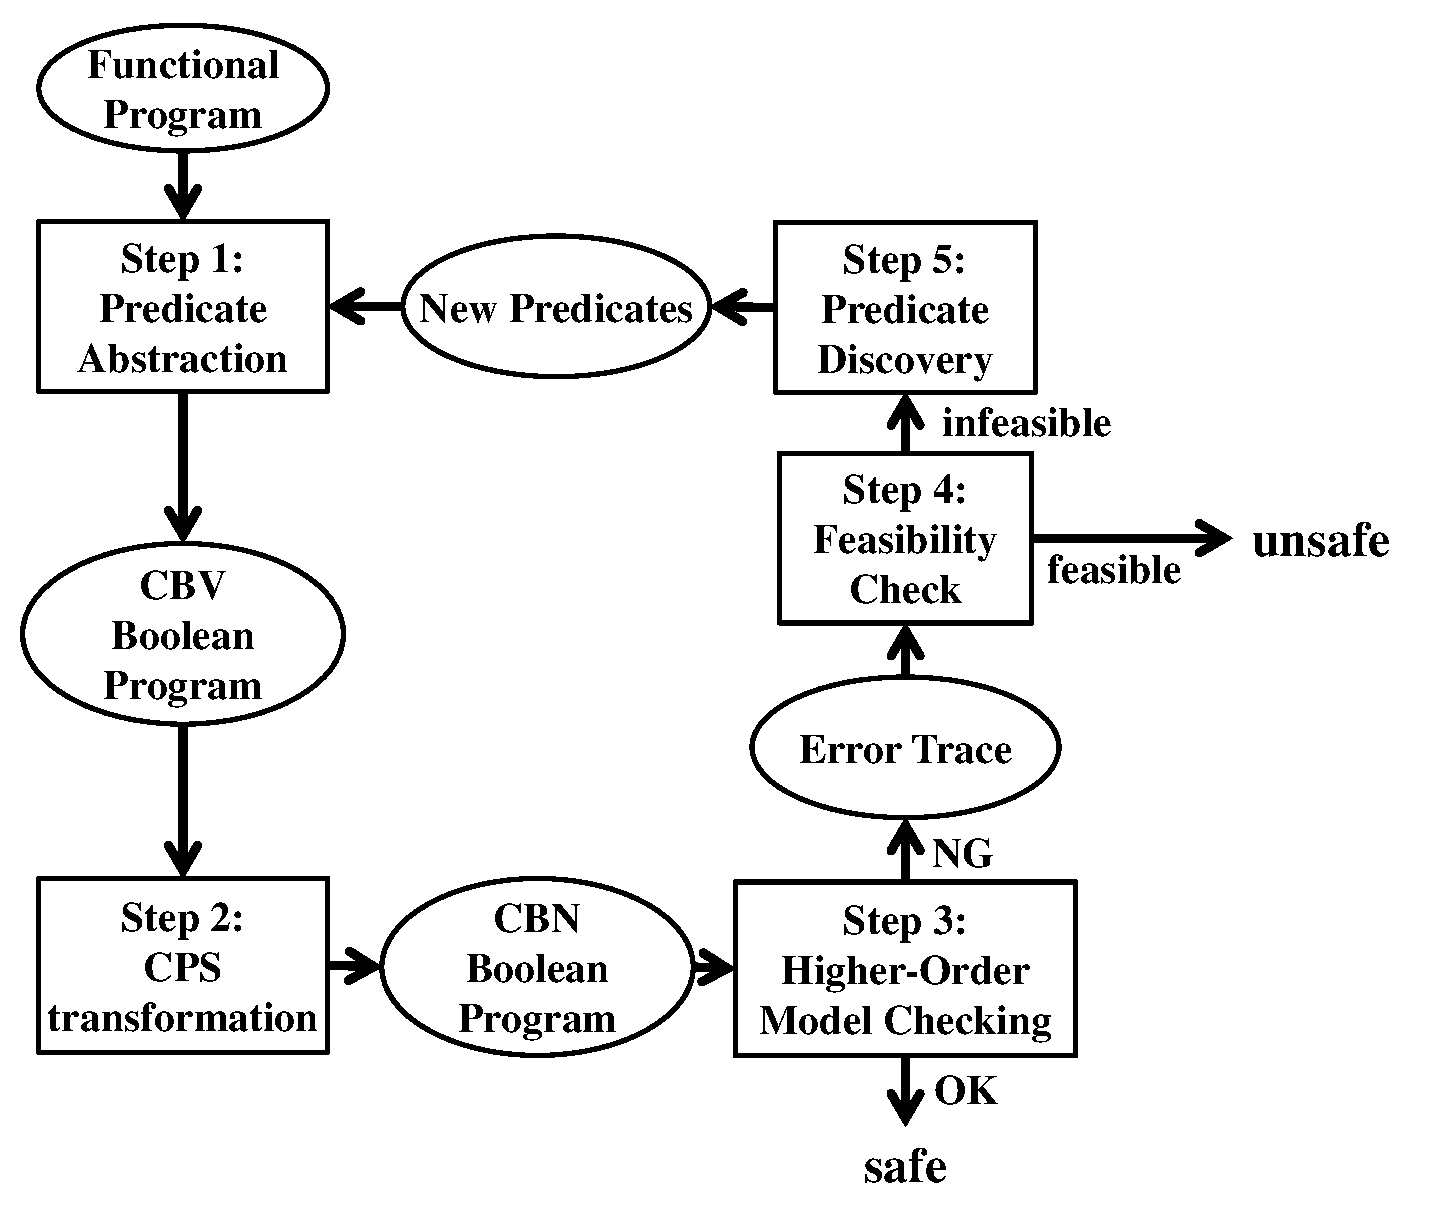
\includegraphics[scale=0.35]{overall.eps}
\caption{Higher-Order Model Checking with Predicate Abstraction and CEGAR}
\label{fig:cegar}
\end{figure}

First, for predicate abstraction, it is unreasonable to use the same set 
of predicates for all the integer variables. For example, let us modify 
the program above into the following program \(M_2\):
\begin{verbatim}
let f x g = g(x+1) in let h y = assert(y>0) in
let k n = if n>=0 then f n h else () in k(randi())
\end{verbatim}
Then, the predicate \(\lambda \nu.\nu\geq 0\) should be used for 
\texttt{x}, while \(\lambda \nu.\nu>0\) should be used for \texttt{y}. 
We should consistently use predicates; for example, with the choice of 
the predicates above, \verb|g|'s argument should be abstracted by using 
\(\lambda \nu.\nu>0\), rather than \(\lambda \nu.\nu\geq 0\). We use 
\emph{types} (called \emph{abstraction types}) to express which 
predicate should be used for each variable. For example, for the above 
program, the following abstraction types are assigned to \(f\), \(h\), 
and \(k\):
\[
\begin{array}{l}
f\COL \ITint{\lambda \nu.\nu\geq 0} \ra (\ITint{\lambda \nu.\nu> 0} \ra \TUNIT) \ra \TUNIT\\
h \COL \ITint{\lambda \nu.\nu> 0} \ra \TUNIT\qquad
%%k\COL \ITint{\lambda \nu.\nu>0}\ra\TUNIT
k\COL \ITint{\,}\ra\TUNIT
\end{array}
\]
The type of \(f\) means that the first argument of \(f\) should be an 
integer abstracted by the predicate \(\lambda \nu.\nu\geq 0\), and the 
second argument be a function that takes an integer abstracted by the 
predicate \(\lambda \nu.\nu>0\) as an argument and returns a unit 
value.\footnote{Here, abstraction types should not be confused with 
refinement types~\cite{Xi1999}; the abstraction type of a term only 
tells how the term should be abstracted, not what are possible values of 
the term. For example, integer \(3\) can have type \(\INT[\lambda 
\nu.\nu<0]\) (and it will be abstracted to the boolean value 
\textit{false}).} By using these abstraction types, the problem of 
checking that predicates are consistently used boils down to a type 
checking problem. For example, the standard rule for application:
\[
\frac{\Gamma \p M: \tau_1 \ra \tau_2\andalso \Gamma\p N:\tau_1}
{\Gamma\p M N: \tau_2}
\]
%%\infrule{\Gamma \p M: \tau_1 \ra \tau_2\andalso \Gamma\p N:\tau_1}
%%  {\Gamma\p M N: \tau_2}
ensures that \(N\) is abstracted using the predicates expected by the 
function \(M\); there is no such case that an abstraction of function 
\(M\) expects a value abstracted by using the predicate \(\lambda 
\nu.\nu>0\) but the actual argument \(N\) is abstracted by using 
\(\lambda \nu.\nu\geq0\).

A further twist is necessary to deal with multi-ary predicates.
For example, consider the following modified version \(M_3\):
\begin{verbatim}
let f x g = g(x+1) in let h z y = assert(y>z) in
let k n = if n>=0 then f n (h n) else () in
   k(randi())
\end{verbatim}
The variable \texttt{y} should now be abstracted by using %%the predicate 
\(\lambda \nu.\nu>\texttt{z}\), which 
depends on the value of \texttt{z}. Thus, %%the abstraction types introduced above should be \emph{dependent} types.
the above program should be abstracted by using the following \emph{dependent} abstraction types:
\[
\begin{array}{l}
f\COL (x\COL\ITint{\,} \ra (w\COL\ITint{\lambda \nu.\nu> x} \ra \TUNIT) \ra \TUNIT) \\
h\COL (z\COL\ITint{\,} \ra y\COL\ITint{\lambda \nu.\nu> z} \ra \TUNIT)\qquad
k\COL \ITint{\,}\ra\TUNIT
\end{array}
\]
Here, please note that the types of the second arguments of \(f\) and 
\(h\) refer to the values of the first arguments. Thus, our type system 
for ensuring the consistency of predicates is actually a \emph{dependent} 
one. A predicate abstraction algorithm is then formalized as a 
type-directed transformation relation \(\Gamma \p M:\tau \Rightarrow e\) 
based on the dependent abstraction type system, where \(M\) is a source 
program and \(e\) is an abstract program.\footnote{To avoid the 
confusion, we call dependent abstraction types just \emph{abstraction 
types} below. We use the term ``dependent types'' to refer to ordinary 
dependent types 
%%(such as
%%\(x\COL\rtbase{\nu}{\INT}{\nu>0}\ra \rtbase{\nu}{\INT}{\nu>x}\), which describe functions that
%%a positive integer \(x\) as input and returns an integer greater than \(x\))
used for expressing refinement of simple types.}

%\koba{Below, we should be careful about what we mean by ``dependent type system''.
%Should we instead use the word ``refinement type system''?}
%
The predicate abstraction mentioned above is sound in the sense that if 
an abstract program is safe (i.e., does not reach \texttt{fail}), so is 
the source program. Further, we can show that it is relatively complete 
with respect to a dependent (refinement) intersection type 
system~\cite{Terauchi2010}: If a source program is typable in the 
dependent intersection type system, our predicate abstraction can 
generate a safe abstract boolean program by using certain abstraction 
types.
%% containing the atomic predicates occurring in the dependent intersection types.
This means that, as long as suitable predicates are provided (by a user 
or an automated method like the CEGAR discussed below), the combination 
of our predicate abstraction and higher-order model checking has at 
least the same verification power as (and actually strictly more 
expressive than, as discussed later: see 
Remark~\ref{rem:more-expressive-than-deptype} in Section~\ref{sec:pred}) 
the dependent intersection type system. Here, note that we need only 
atomic predicates used in the dependent types; higher-order model 
checking can look for arbitrary boolean combinations of the atomic 
predicates as candidates of dependent types. Thus, this part alone 
provides a good alternative to Liquid types~\cite{Rondon2008}, which 
also asks users to provide templates of predicates, and infers dependent 
types. Thanks to the power of higher-order model checking, however, our 
technique can infer dependent, \emph{intersection} types unlike Liquid 
types.
%(This point is discussed in more detail later. )


We now discuss the CEGAR part. Given an error path of an abstract 
boolean program, we can find a corresponding (possibly infeasible) error 
path of the source program. Whether the error path is feasible in the 
source program can be easily decided by symbolically executing the 
source program along the error path, and checking whether all the 
branching conditions in the path are satisfiable (recall the example 
given earlier). The main question is, if the error path turns out to be 
infeasible, how to find a suitable refinement of abstraction types, so 
that the new abstraction types yield an abstract boolean program that 
does not contain the infeasible error path. This has been well studied 
for first-order 
programs~\cite{Ball2001,Ball2002,Ball2005,Heizmann2010,Clarke2003a,Henzinger2002,Henzinger2004},
%
but it is not clear how to lift those techniques to deal with 
higher-order programs.

Our approach to finding suitable abstraction types is as follows.
%%dependent type inference~\cite{Terauchi2010}.
From a source program and its infeasible error path, we first construct 
a \emph{straightline higher-order program} (abbreviated to SHP) that 
exactly corresponds to the infeasible path, and contains neither 
recursion nor conditional branches. In the case of the program \(M_3\) 
above, this is easily obtained, as follows:
\begin{verbatim}
let f1 x g = g(x+1) in let h1 z y = assert(y>z) in
let k1 n = assume(n>=0); f1 n (h1 n) in k1(c)
\end{verbatim}
Here, \texttt{c} is a constant, and \(\texttt{assume}(b)\) evaluates 
\(b\), and proceeds to the next instruction only if \(b\) is true. (But 
unlike \texttt{assert}, it is not reduced to \texttt{fail} even if \(b\) 
is false.) For general programs that contain recursions, the 
construction is more involved: see Section~\ref{sec:cegar}.
%%as shown in Section~\ref{sec:cegar}, a function in the source program
%%may need to be duplicated (i.e., for each function \(f\) in the source program,
%%there may be more than one corresponding function \(f_1,\ldots,f_k\)).

For SHP, a standard dependent (refinement) type system is sound and 
\emph{complete}, in the sense that a program does not reach \texttt{fail} 
if and only if the program is typable in the type system. Further, (a 
sub-procedure of) previous algorithms for inferring dependent types 
based on interpolants~\cite{Unno2009,Terauchi2010} is actually complete 
(modulo the assumption that the underlying logic is decidable and 
interpolants can always be computed) for SHP. Thus, we can automatically 
infer the dependent type of each function in the straightline program. 
For example, for the program above, we obtain:
\[
\begin{array}{l}
\texttt{f1}: (\rtfunb{x}{\INT}
{\rtfun{(\rtfunb{y}{\rtbase{\nu}{\INT}{\nu>x}}{\TUNIT})}{\TUNIT}}) \\
\texttt{h1}: (\rtfunb{z}{\INT}
        {\rtfunb{y}{\rtbase{\nu}{\INT}{\nu>z}}{\TUNIT}}) \\
\texttt{k1}: (\rtfunb{z}{\INT}{\TUNIT})
\end{array}
\]
Here, the type of \texttt{h1} means that given integers \(z\) and \(y\) 
such that \(y>z\), \(\texttt{h1}\,z\,y\) returns a unit value without 
reaching \texttt{fail}. (These dependent types should not be confused 
with abstraction types: the latter only provides information about how 
the source program should be abstracted.)

We then refine the abstraction type of each function in the source 
program with predicates occurring in the dependent types of the 
corresponding functions in the SHP. For example, given the above 
dependent types, we get the following abstraction types:
%%for the source program:
\[
\begin{array}{l}
\texttt{f}: (x\COL\TINT[\,]\ra (y\COL\TINT[\lambda \nu.\nu>x]\ra \TUNIT)\ra\TUNIT) \\
\texttt{h}: (z\COL\TINT[\,]\ra y\COL \TINT[\lambda \nu.\nu>z]\ra \TUNIT) \qquad
\texttt{k}: \ITint{\,}\ra\TUNIT
\end{array}
\]
We can show that the abstraction types inferred in this manner are 
precise enough, in that the abstract program obtained by using the new 
abstraction types no longer has the infeasible error path. (Thus, the 
so-called ``progress'' property is guaranteed as in CEGAR methods for 
finite-state or pushdown model checking.)

%%%From a source program and a spurious 
%%%For first-order programs, 
%%%\koba{Rewrite the paragraph below, to reflect the new CEGAR method.
%%%Also, mention somewhere in the introduction about the properties satisfied by predicate abstraction
%%%and cegar.}
%%%From the simple types of a source program, one can first obtain a ``template'' of
%%%abstraction types. For example, for the last program above, we obtain:
%%%\[
%%%\begin{array}{l}
%%%\hspace*{-.5cm}f\COL (x\COL\ITint{\lambda x.\seq{P_1}(x)}) \ra (w\COL\ITint{\lambda y.\seq{Q_1}(x,y)} \ra \TUNIT) \ra \TUNIT\\
%%%h \COL (z\COL\ITint{\lambda x.\seq{P_2}(x)}) \ra (y\COL\ITint{\lambda y.\seq{Q_2}(z,y)}) \ra \TUNIT\\
%%%n\COL \ITint{\lambda n.\seq{P_3}(n)}
%%%\end{array}
%%%\]
%%%Here, \(\lambda x.\seq{P_i}(x)\) represents a sequence of predicates 
%%%\(\lambda x.P_{i1}(x)\), \(\ldots,\lambda x.P_{ik}(x)\).
%%%The goal of CEGAR is to find, from a counterexample, predicates that should occur 
%%%in the sequences of predicates above.
%%%For that purpose, we can use an interpolating theorem prover, following the interpolant-based technique
%%%for CEGAR in finite state model checking~\cite{Henzinger2004}.
%%%For formulas \(P\) and \(Q\) such that \(P\land Q\) is unsatisfiable,
%%% a \emph{Craig interpolant} of \(P\) and \(Q\) is a formula
%%%\(R\) such that \(P\IMPLY R\) and \(R\IMPLY \neg Q\), with \(\FV{R}\subseteq \FV{P}\cap \FV{Q}\).
%%%Intuitively, \(R\) is a simple justification of why \(P\land Q\) is unsatisfiable. For example,
%%%\(R \equiv x>0\) is an interpolant of \(P \equiv x+y>0 \land y<0\) and 
%%%\(Q \equiv x+z<0 \land z=1\); it is a \emph{simple} justification
%%% in the sense that it refers to only the variables common between the two formulas.
%%%
%%%To see how interpolants can be used in CEGAR, let us consider 
%%% the first program \(M_1\) and the infeasible error path (2).
%%%From the infeasible error path, we get the following sequence of constraints, each of which corresponds to 
%%%a branch condition or a variable binding.
%%%\[
%%%n>0; x=n; y=x+1; \neg(y>0)
%%%\]
%%%Let us cut the above sequence of constraints into \(C_1=\set{n>0,x=n,y=x+1}\) and \(C_2=\set{\neg(y>0)}\).
%%%Note that \(C_1\land C_2\) is unsatisfiable. %%, in other words, \(\forall x,y,n.(\land C_1 \implies \neg (\land C_2))\) holds.
%%%By using an interpolating theorem prover~\cite{Beyer2008,McMillan2005}, one can obtain \(y>0\) as an interpolant of \(\land C_1\) and 
%%%\(\land C_2\). We can use this as a predicate for abstracting \(y\). 
%%%By cutting the sequence of constraints above in other positions, one can also get \(n>0\) and \(x>0\) as interpolants.
%%%Thus, we can use these predicates to abstract the first program.
%%%This idea is basically the same as the interpolant-based CEGAR for imperative programs~\cite{Henzinger2004}.
%%%
%%%A further twist is, however, required for finding predicates in higher-order model checking.
%%%Recall the program \(M_3\). Using the coarsest abstraction, we get the following false error path:
%%%\[
%%%\begin{array}{l}
%%%\texttt{if n>0 then f n (h n) else ()}\red_{n>0} \texttt{f n (h n)}\\
%%%\red \texttt{h n (n+1)} \red \ASSERT{\texttt{(n+1>n)}} \red_{\neg(n+1>n)} \FAIL \\
%%%\hfill\qquad {\cdots(3)}
%%%\end{array}
%%%\]
%%%The corresponding sequence of constraints, representing branch conditions and variable bindings, is:
%%%\[
%%%n>0;\, x=n;\, g=h\, n;\, z=n;\, y=n+1;\, \neg(n+1>n).
%%%\]
%%%From this sequence, however, it is not clear how to extract predicates
%%%that should be used in the template of abstraction type of \(f\):
%%%\[
%%%(x\COL\ITint{\lambda x.\seq{P_1}(x)}) \ra (w\COL\ITint{\lambda w.\seq{Q_1}(x,w)} \ra \TUNIT) \ra \TUNIT
%%%\]
%%%First, the above constraints contain an equality \(g=h\,n\) on functions.
%%%Second, we need to find binary predicates \(\seq{Q_1}(x,w)\) that co-relate \(x\) and \(w\), but
%%%\(w\) does not occur in the sequence above.
%%%In Section~\ref{sec:cegar}, we show (i) how to systematically generate, from an infeasible error path,
%%%constraints (on first-order variables, not on function variables)
%%% that contain information about the co-relations on variables needed in the template of abstraction types,
%%%and (ii) how to re-arrange the constraints so that interpolating theorem provers can be used
%%%to find suitable predicates.
%%%
%%%As mentioned above, our techniques of predicate abstraction and CEGAR for higher-order model checking
%%%are non-trivial extensions of those for finite state or pushdown model checking.

Based on the predicate abstraction and CEGAR techniques mentioned above, 
we have implemented a prototype verifier for (simply-typed) higher-order 
functional programs with recursion and integer base types, and tested it 
for several programs.

Our contributions include: (i) the formalization of predicate 
abstraction for higher-order programs, based on the novel notion of 
abstraction types, (ii) the formalization of CEGAR for higher-order 
programs, based on the novel notion of SHP and reduction of the 
predicate discovery problem to dependent type inference, (iii) 
theoretical properties like the relative completeness of our method with 
respect to a dependent intersection type, the progress property, etc., 
and (iv) the implementation and preliminary experiments.
%%that shows the feasibility of our method (at least for small programs).
%%, despite the extremely high worst-case complexity of higher-order model checking.

The rest of this paper is structured as follows. Section~\ref{sec:lang} 
introduces the source language, and Section~\ref{sec:boolean} introduces 
a language of higher-order boolean programs, and reviews the result on 
higher-order model checking.
%%a higher-order functional programming language with recursion and integer base types
%%as the target of our verification framework.
%%Section~\ref{sec:boolean} introduces a language of higher-order boolean programs, and reviews the result
%%on higher-order model checking (restated for higher-order boolean programs, instead of recursion schemes).
Sections~\ref{sec:pred} and \ref{sec:cegar} respectively formalize 
predicate abstraction and CEGAR for higher-order programs. 
Section~\ref{sec:experiment} reports our prototype implementation and 
preliminary experiments. Section~\ref{sec:related} discusses related 
work, and Section~\ref{sec:conc} concludes.
\iffull
\else
For the space restriction, proofs are omitted, which are available in a 
full version~\cite{Kobayashi2011}.
\fi

%%%In this paper, we propose a verification method ..
%%%
%%%The overall structure of our method is shown in ...
%%%%
%%%For ..., we use a technique called predicate abstraction, which is originally proposed by \cite{Graf1997}.
%%%Translate a program that manipulates infinite data domains 
%%%into a Boolean program whose event sequences over-approximate those of 
%%%the original program.
%%%predicate abstraction for first-order programs is proposed by \cite{Ball2005}.
%%%We investigate predicate abstraction for higher-order programs.
%%%%
%%%For higher-order programs, we have two challenges. The first challenge 
%%%is how to specify predicates. problem: variable scope. Solution: To deal 
%%%with the problem, we use a kind of dependent types to specify predicates. 
%%%The second challenge is how to make abstraction of higher-order programs. 
%%%Problem1: relating the actual and formal argumnets and the return value 
%%%for abstracting higher-order function calls. Solution: type-directed 
%%%translation. especially, type coercions. problem2: cost for computing 
%%%best possible abstraction. solution: ???.
%%%
%%%%
%%%The counterexample-guided abstraction refinement (CEGAR).
%%%Problem: variable scope?? solution: constraint partitioning?
%%%
%%%We overview our method by using the following example: \todo{use a 
%%%practical, higher-order, and simple example}
%%%%
%%%\todo{summation of f(0), ..., f(n)?}
%%%
%%%The rest of the paper is organized as follows. ...

%\section{Background: Predicate Abstraction and CEGAR for Higher-order Model Checking}
\label{sec:model-check}
%\memo{Explanation of previous work}
%\cc{
%A source program is translated into a higher-order program with integers
%by encoding recursive data structures. 
%The language for programs with integers is essentially the same as the source
%language in the previous section, except that it has no list constructors and destructors.
%}
We use our previous verification framework for higher-order
programs with integers~\cite{KobayashiPLDI2011}.  This framework is
based on the higher-order model
checking~\cite{Ong2006,KobayashiPOPL2009}, i.e. model checking of
higher-order recursion schemes, with techniques of predicate abstraction
and counter-example guided abstraction refinement for higher-order
functional programs.

Figure~\ref{fig:cegar} shows the overall structure of our previous
method.  We first translate the source program into boolean program by
predicate abstraction.  Here, predicates are given by the notion of
abstraction types.  Abstraction types are simple types with predicates
that is used as how programs are abstracted to boolean programs.  For
example, abstraction type
$\TFun{x\COL\INT[P_1,\dots,P_n]}{r\COL\INT[Q_1,\dots,Q_m]}$ denotes the
return values are abstracted by predicates $Q_1,\dots,Q_m$ assuming
argument are abstracted by predicates $P_1,\dots, P_n$.  We can verify
the abstracted program by using higher-order model checker.
Higher-order model checker, however, cannot be applied directly to the
abstracted program because of the gap between the semantics of the
abstracted program and recursion scheme that has a call-by-name
semantics.  To resolve the gap, we transform the abstracted program into
a CPS program.  The source program is safe if the abstracted program is
safe.  Otherwise, the model checker generates a counterexample for the
abstracted program.  We can find a corresponding concrete error trace,
and we can check the error path is feasible or not in the source program
by symbolic execution.  The source program is unsafe if the error trace
is feasible.  Otherwise, we can know that the abstraction is too coerce
to verify the source program.  We next refine abstraction types to
refute the counterexample, and continue the CEGAR-loop.

We do not show the details of predicate abstraction and CEGAR for higher-order functional programs here.
See the previous paper~\cite{KobayashiPLDI2011} for the details.


%\section{Model Checking for Higher-order Programs with Integers}
%\label{sec:model-check}
%[Introduction of language (of PLDI2011 + pairs.)]
%
%A source program is translated to a higher-order programs with integers
%by encoding lists as functions. The language of essentially the same as the source
%language in the previous section, except that lists constructor and destructor are not in $\LINT$.
%
%[Description of the framework of PLDI2011.]
%
%We can use the verification framework for higher-order programs with integers [refs].


\vspace{-5pt}
\section{Source Language}
\label{sec:language}
In this section, we introduce the source language of our verification method.
%We extend the language for recursive data structures later.
%As mentioned in Section~\ref{sec:intro},
%We formalize the verification method for a language with lists.
%and argue about recursive data structures later.
%Here, we formalize a language for lists. We extend the language for
%recursive data structures later.

The source language is a simply-typed call-by-value higher-order
functional language with recursion and integers (a la ``PCF'') with the
syntax defined as follows:
\[
\begin{array}{lrl}
D\text{ (programs)} &::=& \{f_1 = v_1, \dots, f_n = v_n\} \\
t\text{ (terms)}
  &::=& n \mid x \mid \Abs{x}{t} \mid t_1\ t_2 \mid \Op{v_1,\dots,v_n} \\
 &\mid& \If{t_1}{t_2}{t_3} \mid \FAIL \\
v\text{ (values)} &::=& n \mid x \mid \Abs{x}{t} \\
\end{array}
\]
%  A program consists a set of top-level functions.
The meta-variable $\OP$ ranges over the set of operators over integers.
The expressions are standard except that there is a primitive $\FAIL$
that aborts a program.  We use $\TRUE$ and $\FALSE$ as aliases of $0$
and $1$, and we write $\Assert{t}$ for $\If{t}{0}{\FAIL}$,
$\Let{x}{t_1}{t_2}$ for $(\Abs{x}{t_2})\ t_1$, and $(v_1\ \OP\ v_2)$ for $\Op{v_1,v_2}$.  We
assume that (i) a program is well-typed in the standard simple type system,
where the set of types is given as $\tau ::= \INT \mid \TFun{\tau_1}{\tau_2}$, (ii)
every function in a program $D$ has a function type, and (iii) $D$ contains a
distinguished function symbol $\main \in \set{f_1,\dots,f_n}$ whose type
is $\TFun{\INT}{\INT}$.

%\begin{figure}[t]
%\[
%\begin{array}{lrl}
%D\text{ (programs)} &::=& \{f_1 = v_1, \dots, f_n = v_n\} \\
%t\text{ (terms)}
%  &::=& n \mid x \mid \Abs{x}{t} \mid t_1\ t_2 \mid \Op{v_1,\dots,v_n} \\
% &\mid& \If{t_1}{t_2}{t_3} \mid \FAIL \\
%v\text{ (values)} &::=& n \mid x \mid \Abs{x}{t} \\
%\tau\text{ (types)} &::=& \INT \mid \TFun{\tau_1}{\tau_2} \\
%\end{array}
%\]
%\caption{The syntax of source language}
%\label{fig:source-syntax}
%\end{figure}

The goal of our verification is to check whether $\App{\main}{n}
\not\reds_D \FAIL$ for all integer $n$.

%\begin{figure}[t]
%\begin{minipage}{\widthcoef\textwidth}
%\[
%\begin{array}{lrl}
%D\text{ (programs)} &::=& \{f_1 = v_1, \dots, f_n = v_n\} \\
%t\text{ (terms)}
%  &::=& n \mid x \mid \Abs{x}{t} \mid t_1\ t_2 \mid \Op{v_1,\dots,v_n} \mid \If{t_1}{t_2}{t_3} \\
% &\mid& \FAIL \mid \Pair{v_1}{v_2} \mid \Fst{t} \mid \Snd{t} \mid \NIL \mid \Cons{v_1}{v_2} \\
% &\mid& (\MATCH\ {t_1}\ \WITH\ \NIL \ra {t_2} \mid \Cons{x_1}{x_2} \ra {t_3}) \\
%
%v\text{ (values)}
%  &::=& n \mid \Abs{x}{t} \mid \Pair{v_1}{v_2} \mid \NIL \mid \Cons{v_1}{v_2} \\
%
%E\text{ (eval. ctx.)}
%  &::=& [\,] \mid E\ t \mid \App{\Abs{x}{t}}{E} \mid \If{E}{t_2}{t_3} \mid \Fst{E} \mid \Snd{E} \\
% &\mid& (\Match{E}{t_2}{t_3}) \\
%
%\tau\text{ (types)} &::=& \INT \mid \TFun{\tau_1}{\tau_2} \mid \TPair{\tau_1}{\tau_2} \mid \List{\tau} \\
%\end{array}
%\]
%\end{minipage}
%\caption{The syntax of source language}
%\label{fig:source-syntax}
%\end{figure}


%\begin{figure}[t]
%\begin{minipage}{\textwidth}
%  \infrule[E-Var]{(f,t) \in D}{f \Red{D} t}
%
%\medskip
%
%  \infax[E-App]{\App{(\Abs{x}{M})}{v} \Red{D} [x \mapsto v]t}
%
%\medskip
%
%  \infax[E-Op]{\Op{v_1,\dots,v_n} \Red{D} \Denote{\OP}(v_1,\dots,v_n)}
%
%\medskip
%
%  \infax[E-If-Then]{\If{0}{t_1}{t_2} \Red{D} t_1}
%
%\medskip
%
%  \infrule[E-If-Else]{n \neq 0}{\If{n}{t_1}{t_2} \Red{D} t_2}
%
%\medskip
%
%  \infax[E-Fst]{\Fst{\Pair{v_1}{v_2}} \Red{D} v_1}
%
%\medskip
%
%  \infax[E-Snd]{\Snd{\Pair{v_1}{v_2}} \Red{D} v_2}
%
%\medskip
%
%  \infax[E-Match-Nil]{\Match{\NIL}{t_2}{t_3} \Red{D} t_2}
%
%\medskip
%
%  \infax[E-Match-Cons]{\Match{\Cons{v_1}{v_2}}{t_2}{t_3} \Red{D} t_3[\subst{x_1}{v_1}][\subst{x_2}{v_2}]}
%
%\medskip
%
%  \infrule[E-Context]{t \Red{D} t'}{E[t] \Red{D} E[t']}
%
%\medskip
%
%  \infax[E-Fail]{E[\FAIL] \Red{D} \FAIL}
%\end{minipage}
%\caption{The semantics of source language}
%\label{fig:source-semantics}
%\end{figure}


\vspace{-2pt}
\subsection{Selective Predicate Abstraction}

We introduce an optimization technique for predicate abstraction, called
selective predicate abstraction.
%Selective predicate abstraction improves the precision of abstraction.

The idea of selective predicate abstraction is to apply predicate
abstractions only to a certain set of functions and inline the other
functions.  For example, the program in Figure~\ref{fig:sum} can
be verified by abstracting only \texttt{sum} and \texttt{main} as stated
in Section~\ref{sec:intro}.

We formalize selective predicate abstraction as an extension of the
previous predicate abstraction.  In the previous framework, predicate
abstraction is defined as the relation
$\AbstPLDI{\Gamma}{t}{\sigma}{t'}$ which means that $t$ is abstracted to
$t'$ by using the abstraction type $\sigma$ under the assumption that
each free variable $x$ of $t$ has been abstracted using the abstraction
type $\Gamma(x)$.  Abstraction types are types to express which
predicate should be used to abstract each value.  For example, an
abstraction type $\INT[P_1,\dots,P_n]$ means that a value
$v$ of that type should be abstracted to a tuple $(b_1,\dots,b_n)$,
where $b_i$ denotes whether $P_i(v)$ holds or not.  See our previous
paper~\cite{KobayashiPLDI2011} for details.  We extend the predicate
abstraction relation by adding the set of inlined functions $E$ like
$\Abst{\Gamma}{E}{t}{\sigma}{t'}$.  Here, functions in $E$ are not
abstracted and are inlined in the process of abstraction.

%\begin{alltt}
%let pred x = x - 1
%let f x = assert (pred x > 0)
%let main x = if x > 1 then f x else ()
%\end{alltt}
%let rec succ n = n + 1
%    and check1 f = assert (f 1 = 2); check1 f
%    and check2 f = assert (f 2 = 3); check2 f
%    and main b = if b then check1 succ else check2 succ
%In our previous framework, we need the following abstraction types to verify the program.
%\[
% \mathtt{pred}\COL\TFun{a}{}, \mathtt{f}\COL\TFun{}{}, \mathtt{main}\COL\TFun{}{}
%\]
%This program can be verified by using the following abstraction types,
%which denotes how predicates we should use to abstract each terms:
%\begin{eqnarray*}
%\mathtt{succ} &:& \TFun{\INT[\Abs{x}{x=1}, \Abs{x}{x=2}]}{\INT[\Abs{x}{x=2}, \Abs{x}{x=3}]} \\
%\mathtt{check1} &:& \TFun{(\TFun{\INT[\Abs{x}{x=1}]}{\INT[\Abs{x}{x=2}]})}{\UNIT} \\
%\mathtt{check2} &:& \TFun{(\TFun{\INT[\Abs{x}{x=2}]}{\INT[\Abs{x}{x=3}]})}{\UNIT} \enspace .
%\end{eqnarray*}
%The type of \texttt{succ} means that the return value is abstracted by predicates
%$\Abs{x}{x=2}$ and $\Abs{x}{x=3}$ assuming that the argument is
%abstracted by predicates $\Abs{x}{x=1}$ and $\Abs{x}{x=2}$.  In fact, it
%is sufficient for verification to use abstraction type
%$\TFun{\INT[\Abs{x}{x=1}]}{\INT[\Abs{x}{x=2}]}$ for \texttt{succ} in
%\texttt{check1 succ}, and
%$\TFun{\INT[\Abs{x}{x=2}]}{\INT[\Abs{x}{x=3}]}$ for \texttt{succ} in
%\texttt{check2 succ}.  Moreover, we can infer these types of
%\texttt{succ} from the callee sides (i.e., just using the argument type
%of check1 and check2.)

%We formalize this abstraction, called selective predicate abstraction,
%as an extension of the previous predicate abstraction.
Figure~\ref{fig:abstraction} shows the key rules of the selective
predicate abstraction.  Other rules are the same as the previous
predicate abstraction relation~\cite{KobayashiPLDI2011} except that the
set of inlined functions $E$ is added.  The relation
$\Abst{\Gamma}{E}{t}{\tau}{t'}$ means that $t$ is abstracted to $t'$ by
using the abstraction type $\tau$ under the assumption that each free
variable $x \in \Dom{\Gamma}$ of $t$ has been abstracted using the
abstraction type $\Gamma(x)$ and each free variable $x \in \Dom{E}$ of
$t$ is inlined.
%$E=\set{f_{i_1}=v_{i_1},\dots,f_{i_k}=v_{i_k}}$ is a subset of a
%program.
%A function definition is in E intuitively means the function
%is expanded in the abstraction.
If $E$ is empty, the selective predicate abstraction relation is the same as the
previous predicate abstraction.

%\begin{equation*}
%V_{D_1,D_2} = \{f \mid (f,t) \in (D_1 \cup D_2)\}
%\end{equation*}
%\begin{equation*}
%E_{D_1,D_2} = \{(f,g) \mid (f,t) \in D_2, g \in \FV{t}\}
%\end{equation*}
%$\ExpNRec{D_2}{-}$ terminates if the graph $(V_{D_1,D_2},E_{D_1,D_2})$ is acyclic.

%\begin{eqnarray*}
% \ExpNRec{D}{c} &=& c \\
% \ExpNRec{D}{x} &=& \left\{
%                     \begin{array}{ll}
%                      x              & \quad \text{$(x,t) \notin D$ for any $t$}  \\
%                      \ExpNRec{D}{t} & \quad \text{$(x,t) \in D$}
%                     \end{array}
%                    \right. \\
% \ExpNRec{D}{\App{t_1}{t_2}} &=& \App{\ExpNRec{D}{t_1}}{\ExpNRec{D}{t_2}} \\
% \ExpNRec{D}{\Op{v_1,\dots,v_n}} &=& \Op{\ExpNRec{D}{v_1}, \dots, \ExpNRec{D}{v_n}} \\
%% \ExpNRec{D}{\If{t_1}{t_2}{t_3}} &=& \If{\ExpNRec{D}{t_1}}{\ExpNRec{D}{t_2}}{\ExpNRec{D}{t_3}}
%\end{eqnarray*}

%\begin{figure}[t]
%\begin{minipage}{\textwidth}
%\infax[Exp-Int]
% {\Exp{D}{n}{n}}
%
%\medskip
%
%\infrule[Exp-Var1]
% {x = t \notin D \text{ for any } t}
% {\Exp{D}{x}{x}}
%
%\medskip
%
%\infrule[Exp-Var2]
% {\Exp{D}{t}{t'}}
% {\Exp{D,x=t}{x}{t'}}
%
%\medskip
%
%\infrule[Exp-Op]
% {\Exp{D}{v_i}{v_i'} \text{ for each } i}
% {\Exp{D}{\Op{v_1,\dots,v_n}}{\Op{v_1,\dots,v_n}}}
%
%\medskip
%
%\infrule[Exp-Abs]
% {\Exp{D}{t}{t'}}
% {\Exp{D}{\Abs{x}{t}}{\Abs{x}{t'}}}
%
%\medskip
%
%\infrule[Exp-App]
% {\Exp{D}{t_1}{t_1'} \andalso
%  \Exp{D}{t_2 }{t_2'}}
% {\Exp{D}{\App{t_1}{t_2}}{\App{t_1'}{t_2'}}}
%
%\medskip
%
%\infax[Exp-Fail]
% {\Exp{D}{\FAIL}{\FAIL}}
%
%\medskip
%
%\infrule[Exp-If]
% {\Exp{D}{t_1}{t_1'} \andalso
%  \Exp{D}{t_2}{t_2'} \andalso
%  \Exp{D}{t_3}{t_3'}}
% {\Exp{D}{\If{t_1}{t_2}{t_3}}{\If{t_1'}{t_2'}{t_3'}}}
%\end{minipage}
%\caption{Inline Expansion}
%\label{fig:inlining}
%\end{figure}

\begin{figure}[t]
\begin{minipage}{0.47\textwidth}
\small
\infrule[A-App]
 {x\notin\Dom{E} \andalso \Gamma(x)=(y_1\COL\sigma_1 \to \cdots \to y_n\COL\sigma_n \to\sigma) \\
 \begin{array}{ll}
  \Gamma,y_1:\sigma_1,\dots,y_{i-1}:\sigma_{i-1}\mid E \vdash \\
  \quad v_i \COL [v_1/y_1,\ldots,v_{i-1}/y_{i-1}]\sigma_i \leadsto e_i
 \end{array} \text{for each $i\in\set{1,\ldots,n}$}}
 {\Abst{\Gamma}{E}{\App{x}{\seq{v}}}{[\seq{v}/\seq{y}]\sigma}{
  \Let{y_1}{e_1}{\cdots\Let{y_n}{e_n}{\App{x}{\seq{y}}}}}}

\smallskip

\infrule[A-AppExp]
 {E(x) = \Abs{\seq{x}}{e} \andalso
  \Abst{\Gamma}{E}{[\seq{v}/\seq{x}]e}{\sigma}{e'}}
 {\Abst{\Gamma}{E}{\App{x}{\seq{v}}}{\sigma}{e'}}

%\smallskip
%
%\infrule[A-Let]
%  {\Abst{\Gamma}{E,x=e_1}{e_2}{\sigma}{e_2'}}
%  {\Abst{\Gamma}{E}{\Let{x}{e_1}{e_2}}{\sigma}{e_2'}}

\smallskip

\infrule[A-Prog]
  {\Abst{\Gamma}{E}{v_i}{\Gamma(f_i)}{v_i'} \andalso
   \text{for each $i$ s.t. $f_i \notin \Dom{E}$} \\
   E \subseteq {\set{f_1 = v_1, \dots, f_n = v_n}} \andalso
   \Dom{\Gamma} \cap \Dom{E} = \emptyset}
  {\AbstProg{\Gamma}{E}{\set{f_1 = v_1, \dots, f_n = v_n}}{\set{f_i = v_i' \mid f_i \notin \Dom{E}}}}
\end{minipage}
\caption{Selective Predicate Abstraction}
\label{fig:abstraction}
\end{figure}

Figure~\ref{fig:abst-example} shows a part of the abstraction of the
program shown in Figure~\ref{fig:sum} with $E =
(\mathtt{add}=\Abs{x}{\Abs{y}{x+y}})$.  Due to the restriction of the
source language of previous predicate
abstraction~\cite{KobayashiPLDI2011}, we translated the term
$\App{\App{\mathtt{add}}{x}}{\App{\mathtt{sum}}{(x-1)}}$ to
$\Let{s}{\App{\mathtt{sum}}{(x-1)}}{\App{\App{\mathtt{add}}{x}}{s}}$.
In the abstraction of $\App{\App{\mathtt{add}}{x}}{s}$, \texttt{add} is
inlined since the definition of \texttt{add} is in $E$.

\begin{figure}[t]
\small
\infer{
\begin{array}{rr}
 \Gamma \mid
 E \vdash
 \Let{s}{\App{\mathtt{sum}}{(x-1)}}{\App{\App{\mathtt{add}}{x}}{s}} \COL
 \INT[\Abs{r}{r \geq x}] \leadsto \quad \\
 \Let{s}{\App{\mathtt{sum}}{()}}{t}
\end{array}
}{
\vdots \qquad
 &
\infer{
 \Abst
  {\Gamma'}
  {E}
  {\App{\App{\mathtt{add}}{x}}{s}}
  {\INT[\Abs{r}{r \geq x}]}
  {t}
}{
\infer{
 \Abst
  {\Gamma'}
  {E}
  {x + s}
  {\INT[\Abs{r}{r \geq x}]}
  {t}
}{\vdots}}}

\caption{Abstraction of $\App{\App{\mathtt{add}}{x}}{(\App{\mathtt{sum}}{(x-1)})}$.
 ($*$ is a syntactic sugar for $\Br{\TRUE}{\FALSE}$.
  $\Gamma = x\COL\INT[], \mathtt{sum}\COL(\TFun{y\COL\INT[]}{\INT[\Abs{r}{r \geq y}]}),~ x>0$.
  $\Gamma' = \Gamma,~s\COL\INT[\Abs{s}{s \geq x-1}]$.
  $E = (\mathtt{add}=\Abs{x}{\Abs{y}{x+y}})$.
  $t = \If{s}{\TRUE}{*}$.)}
\label{fig:abst-example}
\end{figure}
%\begin{figure}[t]
%\infer{
% \Abst
%  {\Gamma}
%  {E}
%  {\Let{s}{\App{\mathtt{sum}}{(x-1)}}{\App{\App{\mathtt{add}}{x}}{s}}}
%  {\INT[\Abs{r}{r \geq x}]}{\Let{s}{\App{\mathtt{sum}}{()}}{t}}
%}{
%\infer{
% \Abst
%  {\Gamma}
%  {E}
%  {\App{\mathtt{sum}}{(x-1)}}
%  {\INT[\Abs{r}{r \geq x-1}]}
%  {\App{\mathtt{sum}}{()}}}
% {\vdots}
% &
%\infer{
% \Abst
%  {\Gamma'}
%  {E}
%  {\App{\App{\mathtt{add}}{x}}{s}}
%  {\INT[\Abs{r}{r \geq x}]}
%  {t}
%}{
%\infer{
% \Abst
%  {\Gamma'}
%  {E}
%  {x + s}
%  {\INT[\Abs{r}{r \geq x}]}
%  {t}
%}{\vdots}}}
%
%\caption{Abstraction of $\App{\App{\mathtt{add}}{x}}{(\App{\mathtt{sum}}{(x-1)})}$.
% ($*$ is a syntactic sugar for $\Br{\TRUE}{\FALSE}$.
%  $\Gamma = x\COL\INT[], \mathtt{sum}\COL(\TFun{y\COL\INT[]}{\INT[\Abs{r}{r \geq y}]}),~ x>0$.
%  $\Gamma' = \Gamma,~s\COL\INT[\Abs{s}{s \geq x-1}]$.
%  $E = (\mathtt{add}=\Abs{x}{\Abs{y}{x+y}})$.
%  $t = \If{s}{\TRUE}{*}$.)}
%\label{fig:abst-example}
%\end{figure}

For some $D$ and $E$, there is $D'$ such that
$\AbstProg{\Gamma}{E}{D}{D'}$ as long as there is no cyclic definitions
in $E$ like $\set{f = \Abs{x}{\App{g}{x}},~ g = \Abs{y}{f}}$.
Therefore, one way to decide $E$ is to find a maximal set of the
functions that has no cyclic definitions.
%Therefore, recursive functions
%should be basically in $\Dom{\Gamma}$, and non-recursive functions
%should be in $\Dom{E}$.
Even if $E$ has some functions which are recursive in $D$,
there is $D'$ such that $\AbstProg{\Gamma}{E}{D}{D'}$ in some cases.
For example, the following program can be abstracted with $E = \set{\mathtt{odd} = v_\mathtt{odd}}$.
\vspace{-5pt}
\begin{alltt}
 letrec even x = if x = 0 then true else odd (x-1)
     and odd x = if x = 0 then false else even (x-1)
 let main () = assert (even (n+n))
\end{alltt}
\vspace{-5pt}
The following is the abstraction of the program with $\Gamma =
\mathtt{even}\COL\TFun{\INT[P_e]}{\BOOL},
\mathtt{main}\COL\TFun{\INT[]}{\UNIT}$ where $P_e = \Abs{x}{(x
\mathop{\mathrm{mod}} 2 = 0})$.
\vspace{-15pt}
\begin{alltt}
 letrec even b =
   if (if b then * else false) then true
   else if (if b then false else *) then false
   else even b
 let main () = assert (even b)
\end{alltt}
\vspace{-5pt}
The abstracted program is safe.  For comparison, consider
the case where $\Gamma = \mathtt{even}\COL\TFun{\INT[P_e]}{\BOOL},
\mathtt{odd}\COL\TFun{\INT[]}{\BOOL},
\mathtt{main}\COL\TFun{\INT[]}{\UNIT}$ and $E=\emptyset$ (which
corresponds to our previous approach~\cite{KobayashiPLDI2011} where the predicates for
\texttt{odd} have not been found yet).
\vspace{-5pt}
\begin{alltt}
 letrec even b = if (if b then * else false)
                 then true else odd ()
    and odd () = if * then false else even *
 let main () = assert (even b)
\end{alltt}
\vspace{-5pt}
Since the abstraction of \texttt{odd} is too coarse, the abstracted
\texttt{even} returns a non-deterministic booleans.  Thus, the
abstracted program is unsafe.

We discuss properties of the selective predicate abstraction.
The theorem below states that selective predicate abstraction is sound
in the sense that if the original program fails then so does its
abstracted program.
\begin{theorem}[Soundness of Selective Predicate Abstraction]
\label{thm:abst_sound}
 If $\AbstProg{\Gamma}{E}{D_1}{D_2}$, and
 $\App{\main}{n} \Reds{D_1} \FAIL$, then
 $\App{\main}{n} \Reds{D_2} \FAIL$.
\end{theorem}

%\begin{theorem}
% If $\Abst{\Gamma}{D}{t}{\tau}{t_1}$,
% $\Abst{\Gamma}{D'}{t}{\tau}{t_2}$,
% $D \subseteq D'$,
% $t_1 \reds \FAIL$ then
% $t_2 \reds \FAIL$.
%\end{theorem}

The following property can be proved in the same manner as the soundness
of the previous predicate abstraction~\cite{KobayashiPLDI2011}.
\begin{prop}
 If $\AbstPLDI{\Gamma}{D}{\tau}{D_1}$,
 $\AbstProg{\Gamma}{E}{D}{D_2}$, and
 $\App{\main}{n} \Reds{D_2} \FAIL$, then
 $\App{\main}{n} \Reds{D_1} \FAIL$.
\end{prop}
The proposition above states that selective predicate abstraction is
more precise compared to our previous predicate abstraction.  Here,
$\AbstPLDI{\Gamma}{D}{\tau}{D_1}$ is the predicate abstraction relation in
our previous paper~\cite{KobayashiPLDI2011}.

%As a consequence of the theorem, we can show that selective predicate
%abstraction with higher-order model checking has at least the same
%verification power of the

%\begin{figure}[t]
%\begin{minipage}{\textwidth}
%
%\infrule[Aff-Const]
% {}
% {\AffineT{S}{f}{n}}
%
%\medskip
%
%\infrule[Aff-Var1]
% {f \in S}
% {\AffineT{S}{f}{f}}
%
%\medskip
%
%\infrule[Aff-Var2]
% {f \neq x}
% {\AffineT{S}{f}{x}}
%
%\medskip
%
%\infax[Aff-Op]
% {\AffineT{S}{f}{\Op{v_1,\dots,v_n}}}
%
%\medskip
%
%\infrule[Aff-Abs]
% {\AffineT{S}{f}{t}}
% {\AffineT{S}{f}{\Abs{x}{t}}}
%
%\medskip
%
%\infrule[Aff-App]
% {\AffineT{S_1}{f}{t_1} \andalso
%  \AffineT{S_2}{f}{t_2} \andalso
%  S = S_1 \uplus S_2}
% {\AffineT{S}{f}{\App{t_1}{t_2}}}
%
%\medskip
%
%\infrule[Aff-Fail]
% {}
% {\AffineT{S}{f}{\FAIL}}
%
%\medskip
%
%\infrule[Aff-If]
% {\AffineT{S_1}{f}{t_1} \andalso
%  \AffineT{S_2}{f}{t_2} \andalso
%  \AffineT{S_2}{f}{t_3} \andalso
%  S = S_1 \uplus S_2}
% {\AffineT{S}{f}{\If{t_1}{t_2}{t_3}}}
%
%\medskip
%
%\infrule[Aff-Prog]
% {\AffineT{S_i}{f}{t_i} \texttt{ for each $i$} \andalso
%  \{f\} = \biguplus S_i}
% {\Affine{f}{\{f_1=t_1,\dots,f_n=t_n\}}}
%
%\end{minipage}
%\caption{Definitions of $\Affine{-}{-}$ \memo{Can we define $\Affine{-}{-}$ only in writing?}}
%\label{fig:affine}
%\end{figure}



%\begin{theorem}
% Suppose Let $t$ be a term in program $D \supseteq D'$, there exists $t'$ such that $...$, if
% $\Affine{f_i}{D}$ holds or $t_i$ is closed, for each definition $f_i = t_i$ in $D'$:
%\end{theorem}
%Here, the definition of $\Affine{-}{-}$ is in
%Fig.~\ref{fig:affine}. $\Affine{f_i}{D}$ denotes $f_i$ is occurred at
%most once except that it counts as ones if $f_i$ occurred at most once
%each in the then-part and the else-part of an if-expression.

\vspace{-5pt}
\section{Optimizations}
\label{sec:opt}

This section introduces optimizations for each phase of CPS
transformation (Step 2) and predicate abstraction (Step 1) in
Figure~\ref{fig:cegar}.


\subsection{Selective CPS transformation}
\label{sec:CPS}
%\TODO{Add discussion about the increase of the order of programs}

This section formalizes selective CPS transformation for abstracted
programs.  As stated in Section~\ref{sec:intro}, the idea of the selective
CPS transformation is to distinguish whether a continuation parameter
should be inserted to each expression or not based on whether it has a
side-effect.  When a function application has no side-effects, we need
not insert a continuation.  Here, $\FAIL$,
non-deterministic branch, and non-termination are considered as
side-effects.
%For example, since an
%application of function $\Abs{x}{\Abs{y}{\Assert{x+y}}}$ to a value has
%no side-effects, it can be transformed to CPS by inserting only one
%continuation like $\Abs{x}{\Abs{y}{\Abs{k}{\App{k}{(x+y)}}}}$ instead of
%$\Abs{x}{\Abs{k}{\App{k}{(\Abs{y}{\Abs{k'}{\App{k'}{(x+y)}}})}}}$.

Note that a similar transformation has been proposed by
Nielsen~\cite{Nielsen2001}.  The transformation does not fit our purpose
to translate call-by-value programs into equivalent call-by-name
programs.  A non-terminating program may be transformed into a
terminating (call-by-name) program by their transformation.
%The reason is that programs obtained by their transformation do not
%yield the same results under a call-by-value semantics and a
%call-by-name semantics.  To be more precise, the transformation does not
%treat non-termination as a side-effect.

To decide whether we should insert a continuation or not, we
annotate each function type with a label $\ell \in \{\NC,\IC\}$, like
$\TFunL{\ell}{\tau_1}{\tau_2}$.  A type $\TFunC{\tau_1}{\tau_2}$ means
that we should insert a continuation, and $\TFunN{\tau_1}{\tau_2}$ means
not.

%\begin{example}[Selective CPS Transformation]
%Consider the following program.
%\begin{alltt}
%let apply = \(\lambda\)x.\(\lambda\)f. f x
%let check = \(\lambda\)x.\(\lambda\)y. assert (x = y)
%let main = \(\lambda\)n. apply n (check n)
%\end{alltt}
%We can translated this program into the following program by na\"{\i}ve CPS transformation.
%\begin{alltt}
%let apply = \(\lambda\)x.\(\lambda\)k1. k1 (\(\lambda\)f.\(\lambda\)k2. f x k2)
%let check = \(\lambda\)x.\(\lambda\)k1. k1 (\(\lambda\)y.\(\lambda\)k2. assert (x = y); k2 ())
%let main = \(\lambda\)n.\(\lambda\)k. check n (\(\lambda\)f1. apply n (\(\lambda\)f2. f2 f1 k))
%\end{alltt}
%The order of this program is \emph{fifth}, i.e. the order of \texttt{apply}.
%%\mathtt{apply}\COL\TFun{\INT}{\TFun{(\TFun{(\TFun{(\TFun{\INT}{\TFun{(\TFun{\INT}{\UNIT})}{\UNIT}})}{\TFun{(\TFun{\INT}{\UNIT})}{\UNIT}})}{\UNIT})}{\UNIT}}
%On the other hand, considering the following annotated program,
%\begin{alltt}
%let apply = \(\lambda\sp{\NC}\)x.\(\lambda\sp{\IC}\)f. f x
%let check = \(\lambda\sp{\IC}\)x.\(\lambda\sp{\IC}\)y. assert (x = y)
%let main = \(\lambda\sp{\IC}\)n. apply n (check n)
%\end{alltt}
%we can translate the program into the following \emph{third} order CPS program.
%\begin{alltt}
%let apply = \(\lambda\)x.\(\lambda\)f.\(\lambda\)k. f x k
%let check = \(\lambda\)x.\(\lambda\)k1. = k1 (\(\lambda\)y.\(\lambda\)k. assert (x = y); k ())
%let main = \(\lambda\)n.\(\lambda\)k. check n (\(\lambda\)f. apply n f k)
%\end{alltt}
%\end{example}

%We used the model checker TRecS in our previous verifier.  Described in
%Section~\ref{model-check}, since TRecS is a model checker for
%higher-order recursion scheme, we need CPS transformation to apply TRecS
%to call-by-value programs.  A na\"{\i}ve CPS transformation, however,
%becomes programs complicate and higher-order.
%
%A selective CPS transformation is a CPS transformation that only
%transforms functions with side effects.

We first define the source language of selective CPS transformation.
The language is the same as the one in Section~\ref{sec:language} except: (i) the set
of terms is extended with non-deterministic branch $\Br{t_1}{t_2}$, and (ii)
a label $\ell \in \{\NC,\IC\}$ is attached to each function type, like
$\TFunL{\ell}{\tau_1}{\tau_2}$.

%\begin{eqnarray*}
% t\text{ (terms)} &::=& \cdots \mid \AbsT{x}{\tau}{t} \mid \AbsTC{x}{\tau}{t} \\
% v\text{ (values)} &::=& \cdots \mid \AbsT{x}{\tau}{t} \mid \AbsTC{x}{\tau}{t} \\
% \tau\text{ (types)} &::=& \cdots \mid \TFunC{\tau_1}{\tau_2}
%\end{eqnarray*}

Below, we formalize the selective CPS as a type-based transformation.
Figure~\ref{fig:cps} shows the rules of the selective CPS
transformation.  The relation $\CPS{\Gamma}{t}{\tau}{\ell}{t'}$ means
that a term $t$ is translated to a term $t'$ by using a type $\tau$,
under the assumption that (i) each free variable $x$ of $t$ has been
transformed using the type $\Gamma(x)$, (ii) $t$ may have a side-effect if
$\ell=\IC$, and (iii) $t$ has no side-effect if $\ell=\NC$.
%Here, $\MAbs{x}{t}$ and
%$\MApp{t_1}{t_2}$ are, respectively, application and abstraction that
%will be reduced statically in the translation.

\begin{figure}[tp]
\begin{minipage}{0.47\textwidth}

\infax[CPS-Const]
 {\CPS{\Gamma}{n}{\INT}{\NC}{n}}

\smallskip

\infax[CPS-Var]
 {\CPS{\Gamma,x\COL\tau}{x}{\tau}{\NC}{x}}

\smallskip

\infrule[CPS-Op]
 {\CPS{\Gamma}{v_i}{\INT}{\NC}{v_i'} \quad \text{for each $i \in \set{1,\dots,n}$}}
 {\CPS{\Gamma}{\Op{v_1,\dots,v_n}}{\INT}{\NC}{\Op{v_1',\dots,v_n'}}}

\smallskip

\infrule[CPS-AbsN]
 {\CPS{\Gamma, x\COL\tau_1}{t}{\tau_2}{\NC}{t'}}
 {\CPS{\Gamma}{\Abs{x}{t}}{\TFunN{\tau_1}{\tau_2}}{\NC}{\Abs{x}{t'}}}

\smallskip

\infrule[CPS-AbsC]
 {\CPS{\Gamma, x\COL\tau_1}{t}{\tau_2}{\ell}{t'}}
 {\CPS{\Gamma}{\Abs{x}{t}}{\TFunL{C}{\tau_1}{\tau_2}}{\NC}
  {\Abs{x}{\Abs{k}{\SApp{\ell}{t'}{k}}}}}

\smallskip

\infrule[CPS-AppN]
 {\CPS{\Gamma}{t_0}{\TFunN{\tau_1}{\tau}}{\NC}{t_0'} \quad
  \CPS{\Gamma}{t_1}{\tau_1}{\NC}{t_1'}}
 {\CPS{\Gamma}{\App{t_0}{t_1}}{\tau}{\NC}
  {\App{t_0'}{t_1'}}}

\smallskip

\infrule[CPS-AppC]
 {\CPS{\Gamma}{t_0}{\TFunL{\ell}{\tau_1}{\tau}}{\ell_0}{t_0'} \andalso
  \CPS{\Gamma}{t_1}{\tau_1}{\ell_1}{t_1'}}
 {
 \begin{array}{l}
  \Gamma \p \App{t_0}{t_1} \COL \tau, \IC \leadsto \\
  \qquad \Abs{k}{\SApp{\ell_0}{t_0'}{\Abs{x_0}{\SApp{\ell_1}{t_1'}{\Abs{x_1}{\SApp{\ell}{\App{x_0}{x_1}}{k}}}}}}
 \end{array}}

%\smallskip
%
%\infrule[CPS-AppN]
% {\CPS{\Gamma}{t_0}{\TFunN{\tau_1}{\TFunN{\cdots}{\TFunN{\tau_n}{\tau}}}}{\NC}{t_0'} \andalso
%  \CPS{\Gamma}{t_i}{\tau_i}{\NC}{t_i'} \quad \text{for each $i \in \set{1,\dots,n}$}}
% {\CPS{\Gamma}{\App{\App{\App{t_0}{t_1}}{\dots}}{t_n}}{\tau}{\NC}
%  {\App{\App{\App{t_0'}{t_1'}}{\ldots}}{t_n'}}}
%
%\smallskip
%
%\infrule[CPS-AppC]
% {\CPS{\Gamma}{t_0}{\TFunL{l_1}{\tau_1}{\TFunL{l_{n-1}}{\cdots}{\TFunL{l_n}{\tau_n}{\tau}}}}{l_0}{t_0'} \andalso
%  \CPS{\Gamma}{t_i}{\tau_i}{l_i}{t_i'} \quad \text{for each $i \in \set{1,\dots,n}$}}
% {\CPS{\Gamma}{\App{\App{\App{t_0}{t_1}}{\dots}}{t_n}}{\tau}{\IC}
%  {\Abs{k}{\SApp{l_0}{t_0'}{\Abs{x_0}{\SApp{l_1}{t_1'}{\Abs{x_1}{\cdots\SApp{l_n}{t_n'}{\Abs{x_n}{\App{\App{\App{\App{x_0}{x_1}}{\ldots}}{x_n}}{k}}}\cdots}}}}}}}
%
\smallskip

\infax[CPS-Fail]
 {\CPS{\Gamma}{\FAIL}{\tau}{\IC}{\Abs{k}{\FAIL}}}

\smallskip

\infrule[CPS-IfN]
 {\CPS{\Gamma}{t_1}{\INT}{\NC}{t_1'} \quad
  \CPS{\Gamma}{t_2}{\tau}{\NC}{t_2'} \quad
  \CPS{\Gamma}{t_3}{\tau}{\NC}{t_3'}}
 {\CPS{\Gamma}{\If{t_1}{t_2}{t_3}}{\tau}{\NC}
  {\If{t_1'}{t_2'}{t_3'}}}

\smallskip

\infrule[CPS-IfC]
 {\CPS{\Gamma}{t_1}{\INT}{\ell_1}{t_1'} \quad
  \CPS{\Gamma}{t_2}{\tau}{\ell_2}{t_2'} \quad
  \CPS{\Gamma}{t_3}{\tau}{\ell_3}{t_3'}}
 {\begin{array}{l}
   \CPS{\Gamma}{\If{t_1}{t_2}{t_3}}{\tau}{\IC}{}{\lambda k.\,\mathit{App}^{\ell_1}(t_1,} \\
   \qquad \Abs{m}{\If{m}{\SApp{\ell_2}{t_2'}{k}}{\SApp{\ell_3}{t_3'}{k}}})
  \end{array}}

\smallskip

 \infrule[CPS-Br]
 {\CPS{\Gamma}{t_1}{\tau}{\ell_1}{t_1'} \andalso
  \CPS{\Gamma}{t_2}{\tau}{\ell_2}{t_2'}}
 {
 \begin{array}{l}
  \Gamma \p \Br{t_1}{t_2} \COL \tau, \IC \leadsto \\
  \qquad \Abs{k}{\If{\Br{0}{1}}{\SApp{\ell_1}{t_2'}{k}}{\SApp{\ell_2}{t_3'}{k}}}
 \end{array}}

\smallskip

\infrule[CPS-Prog]
 {v_i \text{ is of the form } \Abs{x_1}{\Abs{x_2}{\dots\Abs{x_j}{t_i}}} \\
  t_i \text{ is not of the form } \Abs{x}{t_i'} \\
  \Gamma(f_i) \text{ is of the form } \TFunL{\ell_1}{\tau_{i1}}{\TFunL{\ell_2}{\tau_{i2}}{\TFunL{\ell_{j-1}}{\cdots}{\TFunC{\tau_{ij}}{\tau}}}} \\
  \CPS{\Gamma}{v_i}{\Gamma(f_i)}{\NC}{v_i'} \quad \text{for each $i \in \set{1,\dots,n}$}}
 {\CPSprog{\Gamma}{\{f_1=v_1,\dots,f_n=v_n\}}{\{f_1=v_1',\dots,f_n=v_n'\}}}

\begin{center}
$\SApp{\NC}{t}{k} = \App{k}{t}$, \quad $\SApp{\IC}{t}{k} = \App{t}{k}$
\end{center}

\end{minipage}
\caption{Selective CPS transformation}
\label{fig:cps}
\end{figure}

%\begin{figure}[htbp]
%\begin{minipage}{\textwidth}
%\infax[CPS-Const]
% {\CPS{\Gamma}{n}{\INT}{\NC}{\Abs{\kappa}{\App{\kappa}{n}}}}
%
%\smallskip
%
%\infax[CPS-Var]
% {\CPS{\Gamma,x\COL\tau}{x}{\tau}{\NC}{\Abs{\kappa}{\App{\kappa}{x}}}}
%
%\smallskip
%
%\infax[CPS-Op]
% {\CPS{\Gamma}{\Op{v_1,\dots,v_n}}{\INT}{\NC}{\Abs{\kappa}{\App{\kappa}{(\Op{v_1,\dots,v_n})}}}}
%
%\smallskip
%
%\infrule[CPS-AbsN]
% {\CPS{\Gamma, x\COL\tau_1}{t}{\tau_2}{\NC}{t'}}
% {\CPS{\Gamma}{\Abs{x}{t}}{\TFunN{\tau_1}{\tau_2}}{\NC}
%  {\Abs{\kappa}{\Abs{x}{\App{t'}{(\Abs{m}{\App{\kappa}{m}})}}}}}
%
%\smallskip
%
%\infrule[CPS-AbsC]
% {\CPS{\Gamma, x\COL\tau_1}{t}{\tau_2}{\IC}{t'}}
% {\CPS{\Gamma}{\Abs{x}{t}}{\TFunC{\tau_1}{\tau_2}}{\NC}
%  {\Abs{\kappa}{\App{\kappa}{(\Abs{x}{\Abs{k}{\App{t'}{(\Abs{m}{\App{k}{m}})}}})}}}}
%
%\smallskip
%
%\infrule[CPS-AppN]
% {\text{$t_0$ is not of the form $\App{\App{\App{f}{t_{00}}}{\ldots}}{t_{0k}}$} \\
%  \CPS{\Gamma}{t_0}{\TFunN{\tau_1}{\TFunN{\cdots}{\TFunN{\tau_n}{\tau}}}}{\NC}{t_0'} \andalso
%  \CPS{\Gamma}{t_i}{\tau_i}{\NC}{t_i'} \quad \text{for each $i \in \set{1,\dots,n}$}}
% {\CPS{\Gamma}{\App{\App{\App{t_0}{t_1}}{\dots}}{t_n}}{\tau}{\NC}
%  {\Abs{\kappa}{\App{\kappa}{(\App{t_0'}{(\Abs{x_0}{\App{t_1'}{(\Abs{x_1}{\cdots(\Abs{x_n}{\App{\App{\App{x_0}{x_1}}{\ldots}}{x_n}})\cdots})}})})}}}}
%
%\smallskip
%
%\infrule[CPS-AppC]
% {\CPS{\Gamma}{t_0}{\TFunL{l_1}{\tau_1}{\TFunL{l_{n-1}}{\cdots}{\TFunC{\tau_n}{\tau}}}}{l}{t_0'} \andalso
%  \CPS{\Gamma}{t_i}{\tau_i}{l_i'}{t_i'} \quad \text{for each $i \in \set{1,\dots,n}$}}
% {\CPS{\Gamma}{\App{\App{\App{t_0}{t_1}}{\dots}}{t_n}}{\tau}{\IC}
%  {\Abs{\kappa}{\App{t_0'}{(\Abs{x_0}{\App{t_1'}{(\Abs{x_1}{\cdots(\Abs{x_n}{\App{\App{\App{\App{x_0}{x_1}}{\ldots}}{x_n}}{(\Abs{r}{\App{\kappa}{r}})}})\cdots})}})}}}}
%
%\smallskip
%
%\infax[CPS-Fail]
% {\CPS{\Gamma}{\FAIL}{\tau}{\IC}{\Abs{\kappa}{\FAIL}}}
%
%\smallskip
%
%\infrule[CPS-If]
% {\CPS{\Gamma}{t_1}{\INT}{l}{t_1'} \andalso
%  \CPS{\Gamma}{t_2}{\tau}{l}{t_2'} \andalso
%  \CPS{\Gamma}{t_3}{\tau}{l}{t_3'}}
% {\CPS{\Gamma}{\If{t_1}{t_2}{t_3}}{\tau}{l}
%  {\Abs{\kappa}{\App{t_1}{(\Abs{m}{\If{m}{\App{t_2'}{\kappa}}{\App{t_3'}{\kappa}}})}}}}
%
%\smallskip
%
%\infrule[CPS-Br]
% {\CPS{\Gamma}{t_1}{\tau}{l_1}{t_1'} \andalso
%  \CPS{\Gamma}{t_2}{\tau}{l_2}{t_2'}}
% {\CPS{\Gamma}{\Br{t_1}{t_2}}{\tau}{\IC}
%  {\Abs{\kappa}{\If{\Br{0}{1}}{\App{t_2'}{\kappa}}{\App{t_3'}{\kappa}}}}}
%
%\smallskip
%
%\infrule[CPS-Prog]
% {\CPS{\Gamma}{v_i}{\Gamma(f_i)}{\NC}{v_i'} \quad \text{for each $i \in \set{1,\dots,n}$}}
% {\CPSprog{\Gamma}{\{f_1=v_1,\dots,f_n=v_n\}}{\{f_1=\App{v_1}{(\Abs{m}{m})},\dots,f_n=\App{v_n}{(\Abs{m}{m})}\}}}
%
%%\begin{eqnarray*}
%% \CPSty{b} &=& b \\
%% \CPSty{\TFunC{\tau_1}{\tau_2}} &=& \TFun{\CPSty{\tau_1}}{\TFun{(\TFun{\CPSty{\tau_2}}{\UNIT})}{\UNIT}} \\
%% \CPSty{\TFun{\tau_1}{\tau_2}} &=& \TFun{\CPSty{\tau_1}}{\CPSty{\tau_2}}
%%\end{eqnarray*}
%\end{minipage}
%\caption{Selective CPS transformatation}
%\label{fig:cps}
%\end{figure}

The rules are designed in such a way that transformed term $t'$ has type
$\CPSty{\tau}$ if $\CPS{\Gamma}{t}{\tau}{N}{t'}$ holds, and the transformed
term $t'$ has type $\TFun{(\TFun{\CPSty{\tau}}{\AT})}{\AT}$ if
$\CPS{\Gamma}{t}{\tau}{C}{t'}$ holds, where $\AT$ is the answer type and
$\CPSty{\tau}$ is defined by:
\vspace{-5pt}
\[
\begin{array}{rcl}
 \CPSty{\INT} &=& \INT \\
 \CPSty{\TFunN{\tau_1}{\tau_2}} &=& \TFun{\CPSty{\tau_1}}{\CPSty{\tau_2}} \\
 \CPSty{\TFunC{\tau_1}{\tau_2}} &=& \TFun{\CPSty{\tau_1}}{\TFun{(\TFun{\CPSty{\tau_2}}{\AT})}{\AT}}
\end{array}
\]

This shows the intuition that a term of a type $\TFunC{\tau_1}{\tau_2}$
should be inserted a continuation, and another term remains in direct
style.

In the rule \rn{CPS-AbsC}, a term $\Abs{x}{t}$ is transformed in a
standard way, i.e. a continuation parameter $k$ is inserted and $t'$,
the CPS version of $t$, is applied to $k$.  On the other hand, in the
rule \rn{CPS-AbsN}, no continuation parameter is inserted and direct
style is preserved.  The rules for applications are similar. In the rule
\rn{CPS-AppC}, a continuation is inserted, but not in the rule
\rn{CPS-AppN}.  In the rule \rn{CPS-Br}, a term $\Br{t_1}{t_2}$ should
be transformed with $\IC$ and a continuation is needed because we need to treat
non-deterministic branch as a side-effect.  In the rule \rn{CPS-Prog},
since an application of a top-level function may cause a side-effect,
non-termination, the function type for the last argument is annotated
with $\IC$.  For the sake of simplicity, regardless of whether functions
are recursive, we consider all the top-level functions may not terminate
conservatively.
%Although this is a na\"{\i}ve way to transform non-terminating terms.
We can avoid redundant insertion of continuations
by some termination analysis.

{
\def\check{\mathtt{check}}
\def\apply{\mathtt{apply}}
\def\assert{\mathtt{assert}}
\def\assertcps{\mathtt{assert}_\mathtt{CPS}}

Figure~\ref{fig:cps-example} shows examples of the selective CPS
transformation.  The examples are the transformations of
$\Abs{x}{\Abs{y}{\assert(x = y)}}$ with type
$\TFunN{\INT}{\TFunC{\INT}{\INT}}$ for (a) and
$\TFunC{\INT}{\TFunC{\INT}{\INT}}$ for (b).
The transformation of $\Abs{y}{\assert(x = y)}$ in (b) is the same as the one in (a).
In (a), there is no need to insert a continuation parameter to the back of $x$.
On the other hand, in (b), a continuation parameter is inserted.

\begin{figure}[tp]
\begin{minipage}{\textwidth}
\begin{minipage}{0.03\textwidth}
(a)
\end{minipage}
\begin{minipage}{0.9\textwidth}
\infer{
\CPS{\Gamma}
     {\Abs{x}{\Abs{y}{t}}}
     {\TFunN{\INT}{\TFunC{\INT}{\INT}}}{\NC}
     {\Abs{x}{\Abs{y}{\Abs{k}{\App{t'}{k}}}}}
}{
\infer{
 \CPS{\Gamma_x}
     {\Abs{y}{t}}
     {\TFunC{\INT}{\INT}}{\NC}
     {\Abs{y}{\Abs{k}{\App{t'}{k}}}}
}{
\infer{
 \CPS{\Gamma_{xy}}
     {t}
     {\INT}{\IC}
     {\Abs{k}{\App{t'}{k}}}
}{
 \CPS{\Gamma_{xy}}{\assert}{\TFunC{\INT}{\INT}}{\NC}{\assertcps}
  &
 \quad \vdots \quad
}}}
\end{minipage}

\begin{minipage}{\textwidth}
\begin{minipage}{0.05\textwidth}
(b)
\end{minipage}
\begin{minipage}{0.9\textwidth}
\infer{
 \begin{array}{r}
 \Gamma \p
 \Abs{x}{\Abs{y}{t}} \COL
 \TFunC{\INT}{\TFunC{\INT}{\INT}}, \NC \leadsto \qquad \\
 \Abs{x}{\Abs{k'}{\App{k'}{(\Abs{y}{\Abs{k}{\App{t'}{k}}})}}}
 \end{array}
}{
\infer{
 \CPS{\Gamma_x}
     {\Abs{y}{t}}
     {\TFunC{\INT}{\INT}}{\NC}
     {\Abs{y}{\Abs{k}{\App{t'}{k}}}}
}{\vdots}}
\end{minipage}
\end{minipage}
\end{minipage}
\caption{Transformations of $\Abs{x}{\Abs{y}{\assert(x =
y)}}$. ($t = \assert(x =y)$, $t' = \assertcps(x =y)$, $\Gamma_x=\Gamma,x\COL\INT$.
$\Gamma_{xy}=\Gamma_x,y\COL\INT$. $\App{\App{\assertcps}{b}}{k}$ asserts
$b$ and returns $\App{k}{()}$)} \label{fig:cps-example}
\end{figure}
}

In the following, we discuss properties of the selective CPS
transformation.  The theorem below states that we can transform
arbitrary simply-typed programs by the selective CPS transformation.
\begin{theorem}
\label{thm:cps_total}
Suppose $D$ is typable in $\Gamma$. There exists $\Gamma'$ and $D'$ such
that $\Gamma = \ElimAnnot{\Gamma'}$ and $\CPSprog{\Gamma'}{D}{D'}$,
where $\ElimAnnot{\Gamma}$ is a function that maps an environment with
annotations into the corresponding environment without annotations.
\end{theorem}
The following theorem states the soundness of the selective CPS
transformation, that the transformed program is reduced to
the same value as the original program.
\begin{theorem}[Soundness of CPS Transformation]
\label{thm:cps_sound}
If $\CPSprog{\Gamma}{D}{D'}$, then the following holds:
$\App{\main}{n} \Reds{D} \FAIL$ if and only if
$\App{\App{\main}{n}}{(\Abs{x}{x})} \Reds{D'} \FAIL$.
\end{theorem}

%\memo{How to infer types and labels?}

\newcommand{\todo}[1]{\textcolor{red}{***ToDo: #1***}}

\newcommand{\INCON}{\ \bot\ }
\newcommand\imply{\Rightarrow}


\newcommand{\aset}[1]{\{{#1}\}}
\newcommand{\aseq}[1]{\langle#1\rangle}
\newcommand{\adseq}[1]{\langle\hspace*{-0.1em}\langle{#1}\rangle\hspace*{-0.1em}\rangle}
\newcommand{\sembrack}[1]{[\hspace*{-0.1em}[#1]\hspace*{-0.1em}]}
\newcommand{\dom}{\mathop\textit{dom}\nolimits}
\newcommand{\ran}{\mathop\textit{ran}\nolimits}
\newcommand{\smallcolon}{\hspace*{-0.2em}:\hspace*{-0.2em}}
\newcommand{\smallless}{\hspace*{-0.2em}<\hspace*{-0.2em}}

\newcommand{\lvec}{\overrightarrow}
\newcommand{\emptyseq}{\varepsilon}
\newcommand{\inttype}{\texttt{int}}
\newcommand{\unittype}{\texttt{unit}}
\newcommand{\booltype}{\texttt{bool}}
\newcommand{\reftype}[2]{\aset{{#1} \mid {#2}}}
\newcommand{\oldreftype}[3]{\aset{{#1} \smallcolon {#2} \mid {#3}}}
\newcommand{\funtype}[3]{{#1}\smallcolon{#2}\rightarrow{#3}}
\newcommand{\sfuntype}[2]{{#1}\rightarrow{#2}}
\newcommand{\univtype}[3]{\forall{#1}\smallcolon{#2}.{#3}}

\newcommand{\univtobind}[1]{\aseq{{#1}}}

\newcommand{\builttype}{{\it type}}
\newcommand{\conjoftype}{{\it conj}}


\newcommand{\ttst}[2]{\texttt{st}\:{#1}\:{\tt in}\:{#2}}
\newcommand{\ttlet}[3]{\texttt{let}\:{#1}\,\texttt{=}\,{#2}\:\texttt{in}\:{#3}}
\newcommand{\ttifndet}[2]{\texttt{if}\:{*}\:{\tt then}\:{#1}\:{\tt else}\:{#2}}
\newcommand{\ttif}[3]{\texttt{if}\:{#1}\:\texttt{then}\:{#2}\:\texttt{else}\:{#3}}
\newcommand{\ttfun}[3]{{#1}\,{#2}\:\texttt{=}\:{#3}}


\newcommand{\ttlam}[2]{\lambda{#1}.{#2}}
\newcommand{\ttfix}[2]{\texttt{fix}\:{#1}.{#2}}
\newcommand{\ttapp}[2]{{#1}\:{#2}}
\newcommand{\ttassert}[1]{\texttt{assert}\:{#1}}
\newcommand{\ttassume}[1]{\texttt{assume}\:{#1}}
\newcommand{\ttfail}{{\sf fail}}
\newcommand{\ttsafe}{{\sf safe}}
\newcommand{\ttmain}{{\tt main}}

\newcommand{\tttrue}{1}
\newcommand{\ttfalse}{0}

\newcommand{\envmapsto}{\mapsto}
\newcommand{\cpstype}{\star}
\newcommand{\weak}{\preceq}

%\newcommand{\wellscoped}[1]{{\it closed}({#1})}
\newcommand{\scopevars}[1]{\textit{sv}({#1})}
\newcommand{\free}[1]{\textit{fv}({#1})}
%\newcommand{\wellscopedp}[2]{{\it closed}_{#1}({#2})}
\newcommand{\latleq}{\preceq}
\newcommand{\cty}[1]{\textit{ty}({#1})}
\newcommand{\sty}[1]{\textit{sty}({#1})}
\newcommand{\tyshape}[1]{\textit{tshape}({#1})}
\newcommand{\utyshape}[1]{\textit{ushape}({#1})}
\newcommand{\abs}[1]{\ddot{#1}}

\newcommand{\reduce}[1]{\rightarrow_{#1}}

\newcommand{\trans}[1]{\textit{tr}({#1})}

\newcommand{\wildcard}{\_}

\newcommand{\wpre}{\textit{wpre}}
\newcommand{\godel}[1]{\lceil#1\rceil}

\newcommand{\basevar}[1]{\underline{#1}}

\newcommand{\evalterm}{\Downarrow_{\it  val}}

\newcommand{\stepfix}{\Psi_{\it wp}}

\newcommand{\wpretype}{{\it wpty}}

\newcommand{\defaultargs}{\lvec{\beta}}

\newcommand{\basedefaultargs}{\lvec{\alpha}}

\newcommand{\args}{{\it args}}

\newcommand{\notargs}{{\it args}^-}

\newcommand{\vdashs}{\vdash^s}

\newcommand{\mochi}{{\sf MoCHi}}
\newcommand{\maxargs}{{\sf maxargs}}

\newcommand{\head}{x_{\it hd}}

\newcommand{\vdashuni}{\vdash_\forall}

\newcommand{\cand}{\textit{cands}}

\newcommand{\cex}{\leadsto}

\newcommand{\pureintexps}{{\it pureExps}}

\newcommand{\CG}[2]{\textit{cgen}\left(#1 \vdash #2\right)}
\newcommand{\CS}[3]{\textit{cgen}\left(#1 \vdash #2 \leq #3\right)}


\section{Predicate Discovery}
\label{sec:refine}

In this section, we propose an extension of our previous predicate
discovery method for higher-order programs used in
MoCHi~\cite{KobayashiPLDI2011}.  First, we briefly overview the previous
method in Section~\ref{sec:prev} and then discuss its limitation in
Section~\ref{sec:limit}. Section~\ref{sec:ext} explains the extension of
the method, which remedies the limitation.

\subsection{Previous Method}
\label{sec:prev}

In MoCHi, predicates for abstracting each term of a given program are
specified as a kind of dependent types called abstraction types.  MoCHi
infers abstraction types automatically in a counterexample-guided manner
(recall Figure~\ref{fig:cegar}): In a CEGAR iteration of MoCHi, if the
predicate abstraction at that point is not precise enough to show the
safety of the original program, an error path of the abstracted program
is returned as a result of higher-order model checking.  If the abstract
error path is infeasible (i.e., not a genuine path of the original
program), MoCHi generates a straightline higher-order program (SHP)
that is safe if and only if the abstract error path is infeasible.
MoCHi then uses an existing method~\cite{Unno2009} to infer refinement
types that witness the safety of the SHP.  Here, to make the inference
context-sensitive and complete as discussed in Section~\ref{sec:intro},
MoCHi ensures the generated SHP to be linear (i.e., each function is
called exactly once) and recursion-free by duplicating and renaming the
functions called multiple times in the infeasible error path (see
\cite{KobayashiPLDI2011} for more details).  Finally, MoCHi extracts
abstraction types from the refinement types, which contain precise
enough predicates to refute the infeasible error path.

The key ingredient of the above predicate discovery procedure is the
refinement type inference method~\cite{Unno2009}, which consists of two
steps: constraint generation and solving.  We review the two steps
respectively in Sections~\ref{sec:cg} and \ref{sec:cs}.

\subsubsection{Constraint Generation}
\label{sec:cg}

\begin{figure}[t]
\begin{alltt}
letrec copy x = if x=0 then 0 else 1 + copy (x-1)
let main n = assert (copy n = n)
\end{alltt}
\caption{A Simplified Version of the Program in Figure~\ref{fig:copy}}
\label{fig:copy2}
\end{figure}

Let us assume that we are given a SHP \(D\) which is typable under a
refinement type system (see, for example, \cite{Unno2009} for the
definition of the system) if and only if the abstract error path is
infeasible.  For example, let us consider the program in
Figure~\ref{fig:copy2}, which is a simplified version of the one in
Figure~\ref{fig:copy}.  In the course of its verification, we may obtain
the following SHP \(D_{\texttt{copy}}\):
\begin{alltt}
 let copy1 x = assume (x<>0); 1 + copy2 (x-1)
 let copy2 x = assume (x=0); 0
 let main n = assume (copy1 n <> n); fail
\end{alltt}
The SHP corresponds to an infeasible error path where the else- and the
then-branches of \(\texttt{copy}\) are respectively taken in the first
and the second function call of \(\texttt{copy}\), and the assertion in
the \(\texttt{main}\) function fails.  Note here that
\(D_{\texttt{copy}}\) is safe (i.e., \texttt{fail} is not reachable),
and hence is typable under the refinement type system.

From a SHP \(D\), we generate Horn-clause-like constraints which are
satisfiable if and only if \(D\) is typable.  To this end, for each
function in \(D\), we prepare a refinement type template with predicate
variables, which act as placeholders of refinement predicates to be
inferred.  We then generate a typing derivation for \(D\) under the type
environment that associates each function with its type template.
Horn-clause-like constraints on the predicate variables are then
extracted from the derivation.  Since the SHP \(D\) is linear and
recursion-free, generated constraints are non-recursive.  This is
desirable since constraint solving of non-recursive Horn clauses over
decidable underlying theories (e.g., linear arithmetic) is decidable.
For the running example \(D_{\texttt{copy}}\), we use the following
templates:\footnote{For the sake of simplicity, we here omit the type
template of \texttt{main} as well as the refinement predicates for the
argument of \texttt{copy1} and \texttt{copy2}.}
\[
\begin{array}{rcl}
%\begin{eqnarray*}
\texttt{copy1}&\COL&(x\COL\TFun{\INT}{\set{\nu\COL\INT \mid P_1(x,\nu)}}) \\
\texttt{copy2}&\COL&(x\COL\TFun{\INT}{\set{\nu\COL\INT \mid P_2(x,\nu)}})
%\end{eqnarray*}
\end{array}
\]
By using them, we obtain the following set \(C_{\texttt{copy}}\) of
constraints:
\[
\begin{array}{rcl}
%\begin{eqnarray*}
x=0 \land y=0 &\imply& P_2(x,y) \\
P_2(x-1,y) \land x\neq0 \land z=1+y &\imply& P_1(x,z) \\
P_1(n,x) &\imply& x=n
%\end{eqnarray*}
\end{array}
\]

%%%We then use the constraint generation algorithm for terms defined in
%%%Figure~\ref{fig:cgen} to obtain constraints.  In the figure,
%%%$\CG{\Gamma}{e}$ returns a pair of a refinement type $\tau$ and a
%%%constraint $\theta$ such that $\Gamma \vdash e : \tau$ is derivable if
%%%and only if $\theta$ is valid. Similarly, $\CS{\Gamma}{\tau_1}{\tau_2}$
%%%returns a constraint $\theta$ such that $\Gamma \vdash \tau_1 \leq
%%%\tau_2$ is derivable if and only if $\theta$ is valid.
%%%%
%%%The algorithm is almost a straightforward modification of the typing and
%%%subtyping rules in Section~\ref{sec:reftypesystem} except that the
%%%application of the subsumption rule is restricted to the acutal argument
%%%of function applications.

%%%\begin{figure*}[tbh]
%%%\begin{eqnarray*}
%%%\CG{\Gamma}{x}
%%%&=&(\reftype{u}{u = x},\top) \quad (\mbox{if}~\sty{x}=\inttype) \\
%%%\CG{\Gamma}{\kappa}
%%%&=&(\Gamma(\kappa),\top) \quad (\mbox{if}~\sty{\kappa} \in \rightarrow) \\
%%%\CG{\Gamma}{c}
%%%&=&(\cty{c},\top) \\
%%%\CG{\Gamma}{\ttlet{x}{e_1}{e_2}}
%%%&=&\mbox{let~}(\sigma,\theta_1)=\CG{\Gamma}{e_1} \\
%%%& &\mbox{let~}(\cpstype,\theta_2)=\CG{\Gamma,x\smallcolon\sigma}{e_2} \\
%%%& &(\cpstype,\theta_1 \land \theta_2) \\
%%%\CG{\Gamma}{\ttapp{e}{x}}
%%%&=&\mbox{let~}(\funtype{y}{\sigma}{\tau},\theta_1)=\CG{\Gamma}{e} \\
%%%& &\mbox{let~}(\sigma',\theta_2)=\CG{\Gamma}{x} \\
%%%& &(\tau[x/y],\theta_1 \land \theta_2 \land \CS{\Gamma}{\sigma'}{\sigma}) \\
%%%\CG{\Gamma}{\ttifndet{e_1}{e_2}}
%%%&=&\mbox{let~}(\cpstype,\theta_1)=\CG{\Gamma}{e_1} \\
%%%& &\mbox{let~}(\cpstype,\theta_2)=\CG{\Gamma}{e_2} \\
%%%& &(\cpstype,\theta_1 \land \theta_2) \\
%%%\CS{\Gamma}{\cpstype}{\cpstype}
%%%&=&\top \\
%%%\CS{\Gamma}{\funtype{x}{\sigma_1}{\tau_1}}{\funtype{x}{\sigma_2}{\tau_2}}
%%%&=&\CS{\Gamma}{\sigma_2}{\sigma_1} \land \CS{\Gamma,x:\sigma_2}{\tau_1}{\tau_2} \\
%%%\CS{\Gamma}{\reftype{u}{\theta_1}}{\reftype{u}{\theta_2}}
%%%&=&\forall u.(\sembrack{\Gamma} \wedge \theta_1) \imply \theta_2  \quad (\mbox{if}~u \notin \free{\sembrack{\Gamma}})
%%%\end{eqnarray*}
%%%\caption{Constraint generation algorithm.}
%%%\label{fig:cgen}
%%%\end{figure*}

\subsubsection{Constraint Solving}
\label{sec:cs}

Given a set \(C\) of non-recursive Horn clauses, our previous constraint
solving algorithm returns a substitution \(\theta\) for predicate
variables in \(C\) such that \(\theta C\) is valid.
%in a backward manner
The algorithm iteratively finds a solution for each predicate variable
\(P\) in \(C\) as follows:  The algorithm first computes equi-satisfiable
constraints \(C_P\) of the following form by eliminating the other
predicate variables in \(C\) than \(P\):
\begin{eqnarray*}
\phi_{P} \imply P(\seq{x}) \qquad
P(\seq{x}) \imply \phi_{P}'
\end{eqnarray*}
Here, \(\FV{\phi_{P}} \cap \FV{\phi_{P}'} \subseteq \set{\seq{x}}\)
always holds.  Intuitively, the predicate \(P(\seq{x})\) represents an
invariant of some subexpression \(e\) in the SHP, where some variable
\(\nu \in\set{\seq{x}}\) represents the value of \(e\) and each variable
in \(\set{\seq{x}} \setminus \set{\nu}\) represents a free variable in
\(e\).  \(\phi_P\) and \(\phi_{P}'\) respectively represent the
strongest condition satisfied by the value \(\nu\) and the weakest
condition on \(\nu\) required by the context of \(e\).
%
The algorithm then computes \(\mathcal{I}(\phi_P,\neg \phi_P')\) as a
solution for \(P(\seq{x})\) with the help of a technique called
interpolation~\cite{McMillan2005,Beyer2008} from automated theorem
proving.  Here, an interpolant \(\mathcal{I}(\phi_1,\phi_2)\) of
\(\phi_1\) and \(\phi_2\) (such that \(\phi_1\) and \(\phi_2\) are
inconsistent) is a formula \(\phi\) that satisfies the following
conditions:\footnote{Note that interpolants of \(\phi_1\) and \(\phi_2\)
are not unique.  Actually, existing theorem
provers~\cite{McMillan2005,Beyer2008} return one of them, which is
denoted by \(\mathcal{I}(\phi_1,\phi_2)\).}
\vspace{-5pt}
\begin{itemize}
\item \(\phi_1\) implies \(\phi\),
\item \(\phi\) and \(\phi_2\) are inconsistent, and
\item \(\FV{\phi} \subseteq \FV{\phi_1} \cap \FV{\phi_2}\).
\end{itemize}
\vspace{-3pt}
%
For the running example \(C_{\texttt{copy}}\), we obtain the following
constraints by eliminating the other predicate variables than \(P_1\):
\[
\begin{array}{rcl}
%\begin{eqnarray*}
x=1 \land y=0 \land x\neq0 \land \nu=1+y &\imply& P_1(x,\nu) \\
P_1(x,\nu) &\imply& \nu=x
%\end{eqnarray*}
\end{array}
\]
We then obtain, for example, the following solution for \(P_1(x,\nu)\):
\begin{eqnarray*}
\mathcal{I}(x=1 \land y=0 \land x\neq0 \land \nu=1+y,\neg \nu=x)
\equiv \nu=x.
\end{eqnarray*}
By substituting this for \(P_1\) in \(C_{\texttt{copy}}\), we get:
\[
\begin{array}{rcl}
%\begin{eqnarray*}
x=0 \land \nu=0 &\imply& P_2(x,\nu) \\
P_2(x,\nu) &\imply& (x+1\neq0 \land z=1+\nu \imply z=x+1)
%\end{eqnarray*}
\end{array}
\]
We then get, for example, the following solution for \(P_2(x,\nu)\):
\[
\begin{array}{rcl}
%\begin{eqnarray*}
&&\mathcal{I}(x=0 \land \nu=0,\neg (x+1\neq0 \land z=1+\nu \imply z=x+1)) \\
&\equiv& \nu=x.
%\end{eqnarray*}
\end{array}
\]
We thus obtain the following refinement types for \(D_{\texttt{copy}}\):
\[
\begin{array}{rcl}
%\begin{eqnarray*}
\texttt{copy1}&\COL&(x\COL\TFun{\INT}{\set{\nu\COL\INT \mid x=\nu}}) \\
\texttt{copy2}&\COL&(x\COL\TFun{\INT}{\set{\nu\COL\INT \mid x=\nu}})
%\end{eqnarray*}
\end{array}
\]

\subsection{Limitation of Previous Method}
\label{sec:limit}

We now explain the limitation of the previous method by using the
program in Figure~\ref{fig:copy}.  Let us consider the following SHP
\(D_{\texttt{cc}}\):
\begin{alltt}
 let copy1 x = assume (x<>0); 1 + copy2 (x-1)
 let copy2 x = assume (x=0); 0
 let copy3 x = assume (x<>0); 1 + copy4 (x-1)
 let copy4 x = assume (x=0); 0
 let main n = assume (copy3 (copy1 n) <> n); fail
\end{alltt}
The SHP corresponds to an infeasible error path where the else-branch of
\(\texttt{copy}\) is taken in the first and the third calls of
\(\texttt{copy}\), the then-branch is taken in the second and the fourth
calls of \(\texttt{copy}\), and the assertion in the \(\texttt{main}\)
function fails.

For the SHP \(D_{\texttt{cc}}\), we use the following type templates:
\[
\begin{array}{rcl}
%\begin{eqnarray*}
\texttt{copy1}&\COL&(x\COL\TFun{\INT}{\set{\nu\COL\INT \mid P_1(x,\nu)}}) \\
%\texttt{copy2}&\COL&(x\COL\TFun{\INT}{\set{\nu\COL\INT \mid P_2(x,\nu)}}) \\
%\texttt{copy3}&\COL&(x\COL\TFun{\INT}{\set{\nu\COL\INT \mid P_3(x,\nu)}}) \\
\vdots\quad &&\qquad\qquad \vdots \\
\texttt{copy4}&\COL&(x\COL\TFun{\INT}{\set{\nu\COL\INT \mid P_4(x,\nu)}})
%\end{eqnarray*}
\end{array}
\]
And, we get the following set \(C_{\texttt{cc}}\) of constraints:
\[
\begin{array}{rcl}
%\begin{eqnarray*}
x=0 \land y=0 &\imply& P_2(x,y) \\
P_2(x-1,y) \land x\neq0 \land z=1+y &\imply& P_1(x,z) \\
x=0 \land y=0 &\imply& P_4(x,y) \\
P_4(x-1,y) \land x\neq0 \land z=1+y &\imply& P_3(x,z) \\
P_1(n,x) \land P_3(x,y) &\imply& y=n
%\end{eqnarray*}
\end{array}
\]

By eliminating the other predicate variables than \(P_3\) (and with some
simplification), we get the following constraints \(C_{P_3}\):
\[
\begin{array}{rcl}
%\begin{eqnarray*}
x=1 \land \nu=1 &\imply& P_3(x,\nu) \\
%P_3(x,\nu) &\imply& (n=1 \land x=1 \imply \nu=n)
P_3(x,\nu) &\imply& (x=1 \imply \nu=1)
%\end{eqnarray*}
\end{array}
\]
Existing interpolating proves such as \cite{Beyer2008} returns the
following solution for \(P_3(x,\nu)\):
\begin{eqnarray*}
%&&\mathcal{I}(x=1 \land \nu=1,\neg (n=1 \land x=1 \imply \nu=n)) \\
\mathcal{I}(x=1 \land \nu=1,\neg (x=1 \imply \nu=1))
\equiv x=1 \land \nu=1.
\end{eqnarray*}
Note here that the solution is specific to the calling context of the
particular function \texttt{copy3}, and cannot be used as a solution for
\(P_2\) and \(P_4\).  We here want to get more general solutions like
\(\lambda (\nu,x).\nu=x\) which are more likely to constitute an
invariant of the function \texttt{copy} in the original program.  For
this purpose, we believe it is desirable to find the same solution (if
possible) for ``related'' predicate variables which represent (possibly
different) refinement predicates for the same argument or return value
of the same function in the original program.  For the running example
\(C_{\texttt{cc}}\), we want to get the same solution for
\(P_1,\dots,P_4\), and \(\lambda (\nu,x).\nu=x\) in fact satisfies this
extra constraint.

\subsection{Extended Method}
\label{sec:ext}

We now explain our extension of the previous method to remedy the
limitation discussed in Section~\ref{sec:limit}.  The extended predicate
discovery method is based on the framework of the previous method
overviewed in Section~\ref{sec:prev}, but the component for refinement
type inference is extended so that it can merge and generalize
information from multiple calling contexts of a function in multiple
infeasible error paths.  This enables MoCHi to infer a general
refinement type of the function that type-checks the multiple calling
contexts, while preserving the path- and context-sensitivity.  In other
words, the extended method generates constraints from multiple
infeasible error paths (see Section~\ref{sec:extcg}), and tries to find
the same solution (if possible) for related predicate variables (see
Section~\ref{sec:extcs}).

\subsubsection{Extensions of Constraint Generation}
\label{sec:extcg}

We extend the previous constraint generation algorithm overviewed in
Section~\ref{sec:cg} as follows.
\vspace{-5pt}
\begin{itemize}
\item For each CEGAR iteration, we generate constraints from multiple
infeasible error paths instead of a single path:  We keep the set
\(\set{\pi_1,\cdots,\pi_n}\) of the infeasible error paths found so far,
generate the set \(C_i\) of Horn clauses for each path \(\pi_i\), and
pass \(C=C_1 \cup \dots \cup C_n\) to the extended constraint solving
algorithm described in Section~\ref{sec:extcs} as an input.
%For example, \todo{}
\item We also construct and pass an equivalence relation \(E\) on the
predicate variables in \(C\) such that \(P\ E\ Q\) if and only if the
predicate variables \(P\) and \(Q\) represent (possibly different)
refinement predicates for the same argument or return value of the same
function in the original program.  For example, we obtain the trivial
equivalence relation \(E_{\texttt{cc}}=\set{P_1,\dots,P_4}
\times\set{P_1,\dots,P_4}\) for \(C_{\texttt{cc}}\).  The constraint
solving algorithm in Section~\ref{sec:extcs} exploits \(E\) to find
general solutions for \(C\).
\end{itemize}
\vspace{-5pt}
Thus, the extended algorithm generates a pair \((C,E)\) of Horn clauses
\(C\) for multiple paths and an equivalence relation \(E\) on the
predicate variables in \(C\) unlike the previous algorithm which
generates only Horn clauses for a single path.  Here, the pair \((C,E)\)
of constraints can be viewed as hierarchical constraints where \(C\)
must be always satisfied and \(E\) should be satisfied if possible.

\subsubsection{Extensions of Constraint Solving}
\label{sec:extcs}

In this section, we extend the previous constraint solving algorithm
overviewed in Section~\ref{sec:cs}.  Given a pair \((C,E)\) of Horn
clauses \(C\) and an equivalence relation \(E\) on the predicate
variables in \(C\), the algorithm returns a substitution \(\theta\) for
the predicate variables in \(C\) such that \(\theta C\) is valid.  A
distinguishing feature of the algorithm is that it tries to find the
same solution for predicate variables related by \(E\) if possible.
This enables the algorithm to obtain general predicates, which are more
likely to constitute invariants. % of the original program.

%%%\begin{figure}
%%%\todo{}
%%%\caption{The Overall Structure of Our Extended Constraint Solving Algorithm}
%%%\label{fig:extcs}
%%%\end{figure}

%%%The overall structure of the algorithm is shown in Figure~\ref{fig:extcs}.
The extended constraint solving algorithm proceeds as follows:
\vspace{-10pt}
\begin{enumerate}
\item Find a set \(S\) of predicate variables which are related by \(E\)
and may have the same solution in \(C\).
\item Find a candidate solution \(\lambda \seq{x}.\phi\) for all
predicate variable \(Q \in S\).
\item Substitute \(\lambda \seq{x}.\phi\) for predicate variables \(S\)
in \(C\) and repeat the entire procedure if the result still contains a
predicate variable.
\end{enumerate}
\vspace{-10pt}

\paragraph{Finding a set \(S\) of predicate variables:}
To find a set of predicate variables that may have the same solution in
\(C\), for each predicate variable \(P\) in \(C\), we compute
constraints \(C_P\) from \(C\) by eliminating the other predicate
variables than \(P\).
%
For the running example \(C_{\texttt{cc}}\), we obtain:
\[
\begin{array}{rcl}
%\begin{eqnarray*}
C_{P_1}&=&\{x=1 \land \nu=1 \imply P_1(x,\nu), \\
&&\ P_1(x,\nu) \imply (\nu=1 \imply x=1)\}, \\
C_{P_2}&=&\{x=0 \land \nu=0 \imply P_2(x,\nu), \\
&&\ P_2(x,\nu) \imply (\nu=0 \imply (x=-1 \lor x=0))\}, \\
C_{P_3}&=&\{x=1 \land \nu=1 \imply P_3(x,\nu), \\
&&\ P_3(x,\nu) \imply (x=1 \imply \nu=1)\}, \\
C_{P_4}&=&\{x=0 \land \nu=0 \imply P_4(x,\nu), \\
&&\ P_4(x,\nu) \imply (x=0 \imply \nu=0)\}.
%\end{eqnarray*}
\end{array}
\]

%%%In general, the least upper bound of some predicate variable may not
%%%exist because the constraint generation algorithm in
%%%Section~\ref{sec:extcg} may generate a Horn clause of the form
%%%\(P(x)\land P(y) \imply \phi\).  Note here that \(P\) occurs twice in
%%%the left hand side of the constraint.  In such a case, the least upper
%%%bound for \(P\) may not exist.

Let \(\set{P_1,\dots,P_m}\) be the set of predicate variables in \(C\).
%which have the least upper bound.
We pick an equivalence class \(S_0 \in \set{P_1,\dots,P_m} / E\) (e.g.,
the largest one), and further classify \(S_0\) by using
\(C_{P_1},\dots,C_{P_m}\) so that predicate variables which never have
the same solution are separated.
%
Formally, we find \(S_1\dots,S_n\) such that:
\begin{itemize}
\item \(S_0 = S_1 \cup \dots \cup S_n\),
\item \(\phi_{P_{i,1}} \lor \dots \lor\phi_{P_{i,\ell_i}}\) implies
\(\phi_{P_{i,1}}' \land \dots \land\phi_{P_{i,\ell_i}}'\) for each \(i
\in \set{1,\dots,n}\), and
\item \(\phi_{P_{i,1}} \lor \dots \lor\phi_{P_{i,\ell_i}} \lor
\phi_{P_{j,1}} \lor \dots \lor\phi_{P_{j,\ell_j}}\) does not imply
\(\phi_{P_{i,1}}' \land \dots \land\phi_{P_{i,\ell_i}}' \land
\phi_{P_{j,1}}' \land \dots \land\phi_{P_{j,\ell_j}}'\) for each \(i,j
\in \set{1,\dots,n}\) such that \(i \neq j\).
\end{itemize}
Here, \(C_{P}=\set{\phi_{P} \imply P(\seq{x}),P(\seq{x}) \imply
\phi_{P}'}\) and \(S_i=\set{P_{i,1},\dots,P_{i,\ell_i}}\).

We then pick some \(S \in \set{S_1,\dots,S_n}\) (e.g., the largest one).
 For the running example \(C_{\texttt{cc}}\), we get
\(S=S_0=S_1=\set{P_1,\dots,P_4}\) since \(\phi_{P_1} \lor \dots
\lor\phi_{P_4}\) implies \(\phi_{P_1}' \land \dots \land \phi_{P_4}'\).

\paragraph{Finding a candidate solution \(\lambda \seq{x}.\phi\) for \(S\):}
We find a single candidate solution \(\lambda \seq{x}.\phi\) for all the
predicate variables \(Q_1,\dots,Q_{\ell} \in S\) by simultaneously
solving \(C_{Q_1},\dots,C_{Q_{\ell}}\) unlike the previous method.
Formally, we find \(\phi\) such that:
\vspace{-5pt}
\begin{itemize}
\item \(\phi_{Q_1} \lor \dots \lor \phi_{Q_{\ell}}\) implies \(\phi\),
\item \(\phi\) implies \(\phi_{Q_1}' \land \dots \land \phi_{Q_{\ell}}'\), and
\item \(\FV{\phi} \subseteq \set{\seq{x}}\).
\end{itemize}
Here, \(C_{Q_i}=\set{\phi_{Q_i} \imply Q_i(\seq{x}),Q_i(\seq{x}) \imply
\phi_{Q_i}'}\).  We can compute such a formula \(\phi\) as an
interpolant \(\mathcal{I}(\phi_{Q_1} \lor \dots \lor
\phi_{Q_{\ell}},\neg (\phi_{Q_1}' \land \dots \land \phi_{Q_{\ell}}'))\)
but the three conditions of interpolants are not always sufficient for
our purpose to find general predicates.  Actually, we want to obtain as
simple interpolant as possible with respect to the number of
disjunctions.
% and conjunctions.
To this end, we propose a new heuristic operator \(\mathcal{J}\) that
combines the interpolation \(\mathcal{I}\) and convex hull operators.
Let us write \(\mathcal{H}(\phi)\) to denote the convex hull of \(\phi\).
 For formulas \(\phi_1\) and \(\phi_2\) (such that \(\phi_1\) and
\(\phi_2\) are inconsistent), the new operator
\(\mathcal{J}(\phi_1,\phi_2)\) is defined as follows:
\[
\mathcal{J}(\phi_1,\phi_2) =
\left\{
\begin{array}{ll}
\mathcal{I}(\mathcal{H}(\phi_1),\mathcal{H}(\phi_2)) & (\mbox{if~}\mathcal{H}(\phi_1) \INCON \mathcal{H}(\phi_2)) \\
\mathcal{I}(\mathcal{H}(\phi_1),\phi_2) & (\mbox{if~}\neg (\mathcal{H}(\phi_1) \INCON \mathcal{H}(\phi_2)) \land \\
&\ \quad \mathcal{H}(\phi_1) \INCON \phi_2) \\
\mathcal{I}(\phi_1,\phi_2) & (\mbox{otherwise})
\end{array}
\right.
\]
Here, we write \(\phi_1 \INCON \phi_2\) to denote that \(\phi_1\) and
\(\phi_2\) are inconsistent.  Note here that the use of the convex hull
operator enables us to eliminate disjunctions in \(\phi_1\) and
\(\phi_2\), which are passed to an interpolating theorem prover.
%the interpolation operator \(\mathcal{I}\).
In the experiments reported in Section~\ref{sec:experiments}, this often
reduced the number of disjunctions in the output of the interpolating
prover, and hence makes the output more likely to constitute invariants.
%
Thus, we use the new operator \(\mathcal{J}\) instead of \(\mathcal{I}\)
to compute \(\lambda \seq{x}. \mathcal{J}(\phi_{Q_1} \lor \dots\lor
\phi_{Q_{\ell}},\neg (\phi_{Q_1}' \land \dots \land\phi_{Q_{\ell}}'))\)
as a candidate solution \(\lambda \seq{x}. \phi\) for all the predicate
variables \(Q_1,\dots,Q_{\ell} \in S\).  For the running example
\(C_{\texttt{cc}}\), we obtain, for example, the following candidate
solution \(\lambda (x, \nu). \phi\) for \(P_1,\dots,P_4\):
%an interpolating prover returned ... in the experiments reported in Section~\ref{sec:experiments}:
\vspace{-5pt}
\[
\begin{array}{rcl}
%\begin{eqnarray*}
\phi&=& \mathcal{J}(\phi_{P_1} \lor \dots \lor \phi_{P_4},\neg (\phi_{P_1}' \land \dots \land \phi_{P_4}')) \\
%&=& \mathcal{I}(\mathcal{H}(\phi_{P_1} \lor \dots \lor \phi_{P_4}),\neg (\phi_{P_1}' \land \dots \land \phi_{P_4}')) \\
&=& \mathcal{I}(\mathcal{H}(x=\nu=0 \lor x=\nu=1),\neg (\phi_{P_1}' \land \dots \land \phi_{P_4}')) \\
&=& \mathcal{I}(0 \leq x=\nu \leq 1,\neg (\phi_{P_1}' \land \dots \land \phi_{P_4}')) \\
&\equiv& x=\nu
%\end{eqnarray*}
\end{array}
\]

\paragraph{Substituting \(\lambda \seq{x}.\phi\) for \(S\) in \(C\):}
We then substitute the candidate solution \(\lambda \seq{x}.\phi\) for
\(S=\set{Q_1,\dots,Q_{\ell}}\) in \(C\).  Note, however, that we cannot
always substitute all the predicate variables in \(S\) with the
candidate solution \(\lambda\seq{x}.\phi\) because \(Q_i\) may depend on
\(Q_j\) for some \(i \neq j\).  For example, let us consider the
following constraints:
\begin{eqnarray*}
x=0 \imply Q_1(x), \quad
Q_1(x) \imply Q_2(x+1), \quad
Q_2(x) \imply 0 \leq x \leq 2
\end{eqnarray*}
From the constraints, we get:
\begin{eqnarray*}
C_{Q_1}&=&\{\nu=0 \imply Q_1(\nu), Q_1(\nu) \imply -1 \leq \nu\leq 1\}, \\
C_{Q_2}&=&\{\nu=1 \imply Q_2(\nu), Q_2(\nu) \imply 0 \leq \nu \leq 2\}.
\end{eqnarray*}
Thus, we obtain, for example, \(\mathcal{J}(\nu=0 \lor \nu=1,\neg (-1
\leq \nu\leq 1 \land 0 \leq \nu \leq 2)) \equiv 0 \leq \nu \leq 1\) as a
candidate solution for \(Q_1(\nu)\) and \(Q_2(\nu)\).  However,
\([\lambda\nu.0 \leq \nu \leq 1/Q_1,\lambda \nu.0 \leq \nu \leq
1/Q_2](Q_1(x) \imply Q_2(x+1))\) is not valid.  Actually, it is only
safe to substitute \(\lambda \nu.0 \leq \nu\leq 1\) for either \(Q_1\)
or \(Q_2\).

Therefore, we find and substitute only a maximal nonempty subset \(M\)
of \(S\) for which we can safely substitute \(\lambda\seq{x}.\phi\) (i.e.,
\(\set{R \mapsto \lambda\seq{x}.\phi \mid R \in M}C\) is equi-satisfiable
with \(C\)).
%
%%%such that \(\lambda\seq{x}.\phi\) is in fact a solution for every predicate variable in \(M\).
%
%%%Formally, we find \(M=\set{R_1,\dots,R_m}\) such that:
%%%\begin{itemize}
%%%\item \(M \subseteq S\),
%%%\item \(\theta[\lambda \seq{x}.\phi/R_1,\dots,\lambda
%%%\seq{x}.\phi/R_m]C\) is valid for some substitution \(\theta\) for
%%%predicate variables, and
%%%\item for any \(R_0 \in S \setminus M\) and \(\theta\) the following
%%%formula is not valid: \(\theta[\lambda \seq{x}.\phi/R_0,\lambda
%%%\seq{x}.\phi/R_1,\dots,\lambda \seq{x}.\phi/R_m]C\).
%%%\end{itemize}
For the running example \(C_{\texttt{cc}}\), it is in fact safe to
substitute the candidate solution \(\lambda (x,\nu). x=\nu\) for
\(P_1,\dots,P_4\) (i.e., \(M=S\)).  As a result of the substitution, all
the predicate variables in \(C_{\texttt{cc}}\) are eliminated.  Thus, we
obtain the following refinement types for \(D_{\texttt{cc}}\):
\[
\begin{array}{rcl}
%\begin{eqnarray*}
\texttt{copy1}&\COL&(x\COL\TFun{\INT}{\set{\nu\COL\INT \mid x=\nu}}) \\
%\texttt{copy2}&\COL&(x\COL\TFun{\INT}{\set{\nu\COL\INT \mid x=\nu}}) \\
%\texttt{copy3}&\COL&(x\COL\TFun{\INT}{\set{\nu\COL\INT \mid x=\nu}}) \\
\vdots\quad &&\qquad\qquad \vdots \\
\texttt{copy4}&\COL&(x\COL\TFun{\INT}{\set{\nu\COL\INT \mid x=\nu}})
%\end{eqnarray*}
\end{array}
\]


%\todo{discuss termination?}

%%%infer a refinement type of each
%%%subexpression \(e\) of an ordinary ML type \(\tau\):
%%%  The method then computes an
%%%interpolant \(\phi\) of \(\phi_{post}\) and \(\phi_{pre}\), and returns
%%%\(\set{\nu:\tau \mid \phi}\) as a refinement type of \(e\).
%
%%%%Thus, the method considers both forward and backward information of \(e\)
%%%%respectively obtained from \(e\) and the context of \(e\).

\section{Language Extensions}
\label{sec:extension}

\vspace{-2mm}

This section formalizes extensions of the target language of
verification.  Our approach is to translate a source program to a
program that has no recursive data structures and no control operators.
The translation is sound and complete.

Figure~\ref{fig:extension} shows the verification framework for recursive data structures and control
operators.
%\begin{enumerate}
% \item Translation of a source program with control operations into a
%       program with no control operations.
% \item Translation of a program with recursive data structures into a program with lists.
% \item Translation of the program with lists into a program with integers.
% \item Verification for higher-order programs with integers based on our previous framework.
%\end{enumerate}
Section~\ref{sec:recdata} formalizes the encoding of recursive data
structures, and Sect.~\ref{sec:control} introduces the extension for
control operations.

\begin{figure}[t]
 \begin{center}
  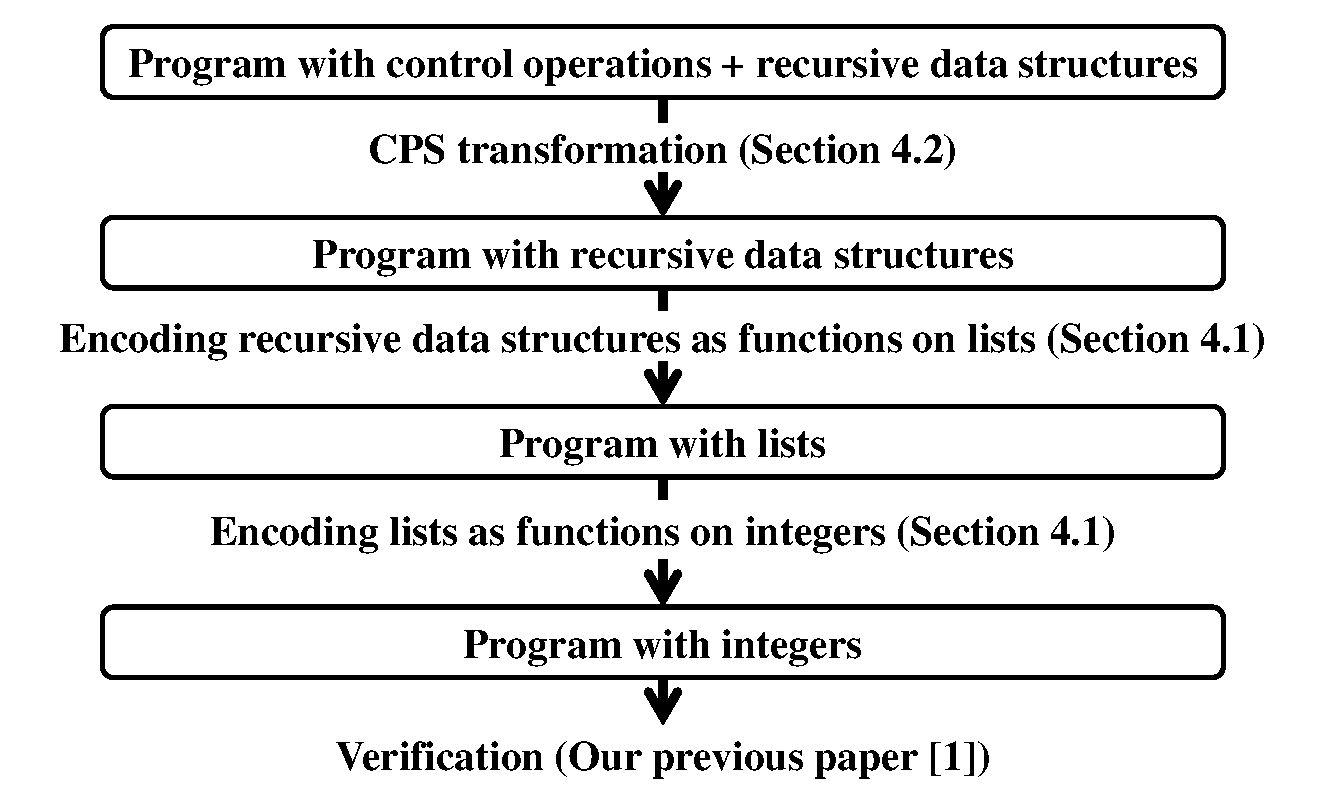
\includegraphics[scale=0.35]{extension.eps}
 \end{center}
\caption{The verification framework for recursive data structures and control operators}
\label{fig:extension}
\end{figure}



\subsection{Functional Encoding of Recursive Data Structures}
\label{sec:recdata}

In this section, we first formalize the encoding of lists, and then we discuss the
extension for user-defined recursive data structures.

%\[
%\begin{array}{lrl}
%D\text{ (programs)} &::=& \{f_1 = v_1, \dots, f_n = v_n\} \\
%t\text{ (terms)}
%  &::=& n \mid x \mid \Abs{x}{t} \mid t_1\ t_2 \mid \Op{v_1,\dots,v_n} \mid \If{t_1}{t_2}{t_3} \\
% &\mid& \FAIL \mid \Pair{v_1}{v_2} \mid \Fst{t} \mid \Snd{t} \mid \NIL \mid \Cons{v_1}{v_2} \\
% &\mid& (\MATCH\ {t_1}\ \WITH\ \NIL \ra {t_2} \mid \Cons{x_1}{x_2} \ra {t_3}) \\
%
%v\text{ (values)}
%  &::=& n \mid \Abs{x}{t} \mid \Pair{v_1}{v_2} \mid \NIL \mid \Cons{v_1}{v_2} \\
%
%E\text{ (eval. ctx.)}
%  &::=& [\,] \mid E\ t \mid \App{\Abs{x}{t}}{E} \mid \If{E}{t_2}{t_3} \mid \Fst{E} \mid \Snd{E} \\
% &\mid& (\Match{E}{t_2}{t_3}) \\
%
%\tau\text{ (types)} &::=& \INT \mid \TFun{\tau_1}{\tau_2} \mid \TPair{\tau_1}{\tau_2} \mid \List{\tau} \\
%\end{array}
%\]

%\begin{figure}[t]
%\begin{minipage}{\widthcoef\textwidth}
%\[
%\begin{array}{lrl}
%D\text{ (programs)} &::=& \{f_1 = v_1, \dots, f_n = v_n\} \\
%t\text{ (terms)}
%  &::=& n \mid x \mid \Abs{x}{t} \mid t_1\ t_2 \mid \Op{v_1,\dots,v_n} \mid \If{t_1}{t_2}{t_3} \\
% &\mid& \FAIL \mid \Pair{v_1}{v_2} \mid \Fst{t} \mid \Snd{t} \mid \NIL \mid \Cons{v_1}{v_2} \\
% &\mid& (\MATCH\ {t_1}\ \WITH\ \NIL \ra {t_2} \mid \Cons{x_1}{x_2} \ra {t_3}) \\
%
%v\text{ (values)}
%  &::=& n \mid \Abs{x}{t} \mid \Pair{v_1}{v_2} \mid \NIL \mid \Cons{v_1}{v_2} \\
%
%E\text{ (eval. ctx.)}
%  &::=& [\,] \mid E\ t \mid \App{\Abs{x}{t}}{E} \mid \If{E}{t_2}{t_3} \mid \Fst{E} \mid \Snd{E} \\
% &\mid& (\Match{E}{t_2}{t_3}) \\
%
%\tau\text{ (types)} &::=& \INT \mid \TFun{\tau_1}{\tau_2} \mid \TPair{\tau_1}{\tau_2} \mid \List{\tau} \\
%\end{array}
%\]
%\end{minipage}
%\caption{The syntax of source language with list}
%\label{fig:list-syntax}
%\end{figure}

\subsubsection{Functional Encoding of Lists}
\label{sec:list}

The idea is to encode a list into a pair of its length and a function that
maps indices to the elements of the list.  For example, the list
$[2;3;5]$ is encoded into the pair $(3,f)$ where $f(0) = 2$, $f(1) = 3$, and
$f(2) = 5$.  The primitive operations \texttt{nil}, \texttt{cons},
\texttt{is\_nil}, \texttt{head}, and \texttt{tail} for lists are defined
as follows.
\begin{alltt}
let nil = (0, fun _ -> fail)
let cons x (len,f) =
  let f' i = if i = 0 then x else f (i-1) in (len+1, f')
let is_nil (len,f) = len = 0
let head (len,f) = if is_nil (len,f) then fail else f 0
let tail (len,f) =
  (if is_nil (len,f) then fail else len-1), fun i -> f (i+1)
\end{alltt}
\texttt{nil} is translated into the pair of length $0$ and the
function that always fails.  \texttt{cons x xs} is translated into the
pair of its length and the function $\{0 \mapsto \mathtt{x}\} \cup \{i \mapsto
f (i-1) \mid i \neq 0\}$ where $f$ is the function part of the encoding of
\texttt{xs}.  \texttt{is\_nil} just checks whether \texttt{len} is 0 or not.
\texttt{head} returns \texttt{f(0)}, i.e. the first
element of the list.  \texttt{tail} returns the pair of
\texttt{(len-1,f')} where $\texttt{f'(i)} = \texttt{f(i+1)}$.

%Since \texttt{f(i)} is the element whose position is \texttt{i} in the
%list, the encoded \texttt{head} returns \texttt{f(0)}, i.e. the $0$-th
%element of the list.  Function \texttt{tail} returns a pair of
%\texttt{(len-1,f')} where $\mathtt{f'(0)} = \mathtt{f(1)}$,
%$\mathtt{f'(1)} = \mathtt{f(2)}$, $\dots$

%Since the original \texttt{head} returns the head of a list,
%the encoded \texttt{head} returns the value

%consider the following
%program.
%\begin{alltt}
%let rec for_all p xs =
%  match xs with [] -> true
%          | x::xs' -> p x && for_all p xs'
%\end{alltt}
%\texttt{for\us{}all p [a1;...;an]} returns a boolean which represents
%whether \texttt{p(a$i$)} holds for every $i$.  We can obtain the
%following list-free program by the encoding mentioned above.
%\begin{alltt}
%let rec for_all p (len,f) =
%  if len = 0 then true
%  else let x = f 0 in
%       let len' = len - 1 in
%       let f' = fun i -> f (i+1) in
%         p x && for_all p (len',f')
%\end{alltt}
%The argument \texttt{xs} is translated into the pair of the length
%\texttt{len} and the function \texttt{f} such that \texttt{f($i$)}
%represents $i$-th element of the list \texttt{xs} (index is 1-origin.)
%The function \texttt{for\us{}all p}, which takes a list, is encoded to a
%higher-order function.  By this encoding, properties of lists are
%translated to ones of functions. For example, a property that
%\texttt{for\us{}all p xs} returns true, i.e. all the elements of
%\texttt{xs} satisfy \texttt{p}, is translated to a property that
%\texttt{f} always returns a positive integer.

This approach has the following advantages.  First, by encoding lists
into functions over integers, we can reuse the predicate
abstraction/discovery for integers.  Second, the encoding induces a
natural predicate abstraction of lists, which is general enough to
subsume various abstractions known in the literature, such as Dillig et
al.'s container abstraction~\cite{Dillig2011}.  In their abstraction
method for aggregate data structures like lists, a list is represented
as $\set{(v_1,P_1), \dots, (v_n,P_n)}$ that means the $j$-th element is
$v_i$ if $P_i(j)$ holds.  For example, $\set{(0,\TRUE)}$ denotes that all
the elements are $0$ and $\set{(1,\Abs{i}{i \mathop{\mathtt{mod}} 2 =
0})}$ denotes that the even indexed elements are $1$.  On the other
hand, by encoding a list as a function, the same information can be
represented as a refinement type $\TFun{(i\COL\INT)}{\set{x\COL\INT\mid
(P_1(i) \to x=v_1) \wedge \dots \wedge (P_n(i) \to x=v_n)}}$.  For
example, $\set{(1,\Abs{i}{i \mathop{\mathtt{mod}} 2 = 0})}$ is
represented as $\TFun{(i\COL\INT)}{\set{x\COL\INT\mid i
\mathop{\mathtt{mod}} 2 = 0 \to x=1}}$.  Moreover, our approach can deal
with list properties like ``the $i$-th element of a list is greater than
$i$,'' which cannot be represented by the container abstraction.  Thus,
our method, i.e., a combination of the encoding and the predicate
abstraction for integers, is strictly more expressive than the container
abstraction.

%\paragraph{Comparison with Dillig et al.'s appoach.}
%Dillig et al.~\cite{Dillig2011} have proposed an automatic technique for
%static reasoning about containers (e.g., maps, lists, and vectors). They
%model containers as functions that map a key to an abstract index that
%is mapped to a value corresponds to the index.  For example, a store
%includes list $[2;3]$ is abstracted as a map $\{\beta \mapsto
%\set{(\AbstLoc{\eta}{i}, \TRUE)}, \AbstLoc{\eta}{i} \mapsto
%\set{(2,i=0),(3,i=1),(\NIL,i \neq 0 \land i \neq 1)}\}$, where $\beta$
%is the memory location that stores the list, and $\AbstLoc{\eta}{i}$ is
%the abstract location indexed with $i$ that represents the list.  In the
%abstract store, $x \mapsto \set{(\pi_1, P_1), \dots, (\pi_n, P_n)}$
%represents that $x$ could have a value $\pi_i$ when $P_i$ holds.  Our
%approach is a generalization of their approach in the following sense:
%\begin{enumerate}
% \item While our abstraction uses arbitrary predicates for container elements,
%       they abstracts container elements to the set of unknown values,
%       integer constants, and locations.
% \item While our abstraction can depend on the index by the form ``if $P_(i)$
%       then $Q(i,v)$'' where $i$ is an index and $v$ is the element at the
%       index $i$, their abstraction can depend on the index only by the form ``if $P_(i)$
%       then $Q(v)$''.
%\end{enumerate}

%Once a target program is translated to a list-free program,
%we can apply our previous verification framework for higher-order programs with integers.

%Figure~\ref{fig:list-translation} shows the definition of the
%translation $\Trans{-}$.  Let $t$ be a list of the form
%$[v_0,\dots,v_{n-1}]$. $\Trans{t}$ denotes the pair of the length $n$ of
%$t$ and the function $\{0 \mapsto v_0, \dots, n-1 \mapsto v_{n-1}\}$
%that maps indices to elements of $t$.  $\NIL$ is translated into the pair of length $0$ and the
%function that always fails.  $\Cons{v_1}{v_2}$ is translated into the
%pair of its length and the function $\{0 \mapsto v_1\} \cup \{i \mapsto
%f (i-1) \mid i \neq 0\}$ where $f$ is the function part of encoding of
%$v_2$.  A pattern match is translated into an if-expression whose
%then-case and else-case respectively correspond to the $\NIL$ and
%$\Cons{x_1}{x_2}$ cases.
%
%\begin{figure}[t]
%\begin{minipage}{\widthcoef\textwidth}
%\[
%\begin{array}{l}
%% \Trans{n} = n \\
%% \Trans{x} = x \\
%% \Trans{\Fix{f}{x}{t}} = \Fix{f}{x}{\Trans{t}} \\
%% \Trans{t_1\ t_2} = \Trans{t_1}\ \Trans{t_2} \\
%% \Trans{\Op{v_1,\dots,v_n}} = \Op{\Trans{v_1}, \dots, \Trans{v_n}} \\
%% \Trans{\If{t_1}{t_2}{t_3}} = \If{\Trans{t_1}}{\Trans{t_2}}{\Trans{t_3}} \\
%% \Trans{\FAIL} = \FAIL \\
%% \Trans{\Pair{t_1}{t_2}} = \Pair{\Trans{t_1}}{\Trans{t_2}} \\
% \Trans{\NIL} = \Pair{0}{\Abs{u}{\FAIL}} \quad (\text{$u$ is fresh}) \\
%
% \Trans{\Cons{v_1}{v_2}} = (\Fst{v_2} + 1, \\
% \qquad \Abs{i}{\If{i-1}{\Trans{v_1}}{\Snd{v_2}\ (i-1)}}) \\
% \quad (\text{$i$ is fresh}) \\
%
% \Trans{\Match{t_1}{t_2}{t_3}} = \\
% \quad \Let{x}{\Trans{t_1}}{} \\
% \quad \Let{len}{\Fst{x}}{} \\
% \quad \Let{f}{\Snd{x}}{} \\
% \qquad \IF\ len\ \THEN\ \Trans{t_2} \\
% \qquad \ELSE\ \Let{x_1}{f\ 0}{}\\
% \qquad\qquad\, \Let{x_2}{\Pair{len - 1}{\Abs{i}{f (i+1)}}}{} \\
% \qquad\qquad\quad \Trans{t_3} \\
% \quad (\text{$x$, $len$, $f$ and $i$ are fresh}) \\
%\end{array}
%\]
%\end{minipage}
%\caption{Encoding of list (excerpt).}
%\label{fig:list-translation}
%\end{figure}

%The theorem below states that the translation $\Trans{-}$ is correct in
%the sense that if a source program fails, so does the translated program, and vice versa.
%\begin{theorem}[Correctness of translation]
%  \label{th:translation-list-correct}
%  Let $t$ be a term in a program $D$.
%  $t \Reds{D} \FAIL$ if and only if $\Trans{t} \Reds{D} \FAIL$.
%\end{theorem}



\subsubsection{Extension for Recursive Data Structures}
We discuss how to encode other recursive data structures.  We
translate programs with recursive data structures into programs with
lists by encoding recursive data structures to functions which map paths
of nodes to labels.  Here, a path and a label are represented as a list
of integers and an integer respectively.  For example, consider binary trees defined
as follows.
\begin{alltt}
type btree = Leaf | Node of btree * btree
\end{alltt}
A binary tree is encoded into a term of the type
$\TFun{\List\INT}{\INT}$.  For example, a binary tree
$\Node{\LEAF}{\Node{\LEAF}{\LEAF}}$ is encoded into a function $\{[]
\mapsto \NODE, [1] \mapsto \LEAF, [2] \mapsto \NODE, [2,1] \mapsto
\LEAF, [2,2] \mapsto \LEAF\}$ where $\LEAF$ and $\NODE$ are defined as
some integers.
Here is another example, the encoding of a pattern matching.
\begin{alltt}
match x with Constr_1(x1, x2, ...) -> t | Constr_2(...) -> ...
\end{alltt}
The expression above is encoded to the following expression.
\begin{alltt}
let Constr_1 = 1 in ... let Constr_n = n in
  match x nil with Constr_1 -> let x1 xs = x (cons 1 xs) in ...
                               let xn xs = x (cons n xs) in t'
                 | Constr_2 -> ...
\end{alltt}
Here, \texttt{t'} is the encoding of \texttt{t}. The pattern matching in
trees is translated to the pattern matching in labels, represented as
integers.  A subterm of a tree is obtained by adding the index to the head of the path.
%\begin{alltt}
%let rec get_child t =
%  match t with
%    Constr(t1,t2)Leaf -> fail
%  | Node(t1,t2) -> (t1, t2)
%\end{alltt}
%This program takes an unlabeled binary tree and returns its children.
%The program is translated into the following program with no recursive
%data structures except lists.
%\begin{alltt}
%let Leaf = 0
%let Node = 1
%let rec get_child t =
%  match t nil with
%    Leaf -> fail
%  | Node ->
%      let t1 xs = t (cons 0 xs) in
%      let t2 xs = t (cons 1 xs) in
%        (t1, t2)
%\end{alltt}

We treat only regular algebraic data types, i.e., the finite combination of sum
types and product types.  When types of recursive data structures are
represented as recursive types, we require that in a recursive type
$\RecType{\alpha}{\tau}$, $\alpha$ does not occur below function type
constructors. For example, $\List{(\TFun{\INT}{\INT})}$ is OK, but
neither $\RecType{\alpha}{\TFun{\alpha}{\INT}}$ nor
$\RecType{\alpha}{\TFun{\INT}{\alpha}}$ is allowed.

%The reason is that the encoding recursive data types generates recursive types again.

%We introduce the language extended with recursive data structures.
%Figure~\ref{fig:rec-syntax} shows the syntax of the language.  The
%meta-variable $\CONSTR$ ranges over the sets of constructor names.
%$\Constr{}{v_1,\dots,v_k}$ is a constructor and $\MatchRec{t}{t_1}{t_k}$
%is a destructor for a type
%$\Constr{1}{\widetilde{\phi_1}} + \ldots + \Constr{k}{\widetilde{\phi_k}}$.
%A program is a pair of function definitions and type definitions
%$\gamma_1=\rho_1, \dots, \gamma_m=\rho_m$.
%A type definition
%$\gamma_1=\Constr{1}{\widetilde{\phi_1}} + \dots + \Constr{k}{\widetilde{\phi_k}}$
%means that type $\gamma$ has
%constructors $\CONSTR_1, \dots, \CONSTR_k$ and the types of the
%arguments of $C_i$ are $\widetilde{\phi_i}$.
%Note that, expressions for pattern matching on lists are distinct
%from ones for pattern matching on recursive data structures.  We restrict the types of the
%constructor arguments, represented by meta-variable $\phi$, to
%$\INT$ or recursive data types for the sake of simplicity.
%
%%We assume that $\gamma$ and $\CONSTR$ are distinct from others.
%
%
%\begin{figure}[t]
%\begin{minipage}{\textwidth}
%\[
%\begin{array}{lrl}
%D\text{ (program)} &::=& \{ f_1=t_1, \dots, f_n=t_n; \gamma_1=\rho_1, \ldots, \gamma_m=\rho_m \} \\
%t\text{ (terms)} &::=& \ldots \mid \Constr{}{\widetilde{v}} \mid (\MatchRec{t}{t_1}{t_k}) \\
%
%\rho\text{ (rec. type)} &::=& \Constr{1}{\widetilde{\phi_1}} + \dots + \Constr{k}{\widetilde{\phi_k}} \\
%\phi &::=& \INT \mid \gamma \\
%\tau\text{ (types)} &::=& \ldots \mid \gamma \\
%\end{array}
%\]
%\end{minipage}
%\caption{The syntax of language extended with recursive data structures}
%\label{fig:rec-syntax}
%\end{figure}
%
%\begin{example}
%A type definition for rose trees is represented as the following.
%\begin{eqnarray*}
% \RTREE &=& \RTNODE(\RTLIST) \\
% \RTLIST &=& \RTNIL() + \RTCONS(\RTREE, \RTLIST)
%\end{eqnarray*}
%%\memo{$\TREE = \NIL() + \NODE(\TREE, \TREE)$}
%\end{example}
%
%
%Figure~\ref{fig:rec-translation} shows the definitions of the translation $\TransRec{D}{-}$.
%$\TransRec{D}{t}$ denotes a function that maps paths to nodes of $t$.
%%Translation of constructors and destructors of lists are trivial, translate recursively.
%%We translate a recursive data $\Constr{}{v_1,\dots,v_n}$ into a function
%%that returns
%$\TransRec{D}{\Constr{}{v_1,\dots,v_n}}$ is a function that returns
%\begin{itemize}
% \item an integer $\TransRec{D}{C}$, correspondence number to $\CONSTR$, for $\NIL$,
% \item $v_k$ for a list whose head is $k$ when $v_k$ has type $\INT$, and
% \item $\App{\TransRec{D}{v_k}}{p}$ for a list that has the form of
%       $\Cons{k}{p}$ when $v_k$ has a recursive data type.
%\end{itemize}
%We translate $\MatchRec{t}{t_1}{t_k}$ into a if-expression that
%checks what is $\App{\TransRec{D}{t}}{\NIL}$, the root node label of
%$t$.  We can obtain the translated value%, the constructor
%argument, to which it bound to variable $x_{ij}$ by
%$\App{f}{(\Cons{i}{\NIL})}$ for $\INT$ and
%$\Abs{p}{\App{f}{(\Cons{i}{p})}}$ for recursive data types.
%%\TODO{add (or rewrite to) more intuitionistic explanation}




%\begin{figure}[t]
%\begin{minipage}{\textwidth}
%\[
%\begin{array}{l}
%% \TransRec{D}{n} = n \\
%% \TransRec{D}{x} = x \\
%% \TransRec{D}{\Fix{f}{x}{t}} = \Fix{f}{x}{\TransRec{D}{t}} \\
%% \TransRec{D}{t_1\ t_2} = \TransRec{D}{t_1}\ \TransRec{D}{t_2} \\
%% \TransRec{D}{\Op{t_1,\dots,t_n}} = \Op{\TransRec{D}{t_1}, \dots, \TransRec{D}{t_n}} \\
%% \TransRec{D}{\If{t_1}{t_2}{t_3}} = \If{\TransRec{D}{t_1}}{\TransRec{D}{t_2}}{\TransRec{D}{t_3}} \\
%% \TransRec{D}{\FAIL} = \FAIL \\
%% \TransRec{D}{\Pair{t_1}{t_2}} = \Pair{\TransRec{D}{t_1}}{\TransRec{D}{t_2}} \\
% \TransRec{D}{\NIL} = \NIL \\
% \TransRec{D}{\Cons{t_1}{t_2}} = \Cons{\TransRec{D}{t_1}}{\TransRec{D}{t_2}} \\
% \TransRec{D}{\Match{t_1}{t_2}{t_3}} = \\
%  \quad \Match{\TransRec{D}{t_1}}{\TransRec{D}{t_2}}{\TransRec{D}{t_3}} \\
%
% \TransRec{D}{\Constr{}{v_1,\dots,v_n}} = \\\qquad
%  \Abs{x}{}\MATCH\ x\ \WITH\ \NIL \ra \TransRec{D}{\CONSTR} \\\qquad\qquad
%  \begin{array}{ll}
%   \mid \Cons{k}{p} \ra & \If{k - 1}{\RecConstr{D}{C}{1}{p}{\TransRec{D}{v_1}}}{} \\
%                        & \If{k - 2}{\RecConstr{D}{C}{2}{p}{\TransRec{D}{v_2}}}{} \\
%                        & \quad \dots \\
%                        & \If{k - n}{\RecConstr{D}{C}{n}{p}{\TransRec{D}{v_n}}}{\FAIL} \\
%  \end{array} \\
% \TransRec{D}{\MatchRec{t}{t_1}{t_k}} = \\
% \quad \Let{f}{\TransRec{D}{t}}{} \\
% \quad \Let{l}{\App{f}{\NIL}}{} \\
% \qquad \If{l - 1}{\RecDestr{D}{\CONSTR_1}{f}{\TransRec{D}{t_1}}}{} \\
% \qquad \If{l - 2}{\RecDestr{D}{\CONSTR_2}{f}{\TransRec{D}{t_2}}}{} \\
% \qquad \quad \dots \\
% \qquad \If{l - k}{\RecDestr{D}{\CONSTR_k}{f}{\TransRec{D}{t_k}}}{\FAIL} \\
%\end{array}
%\]
%\[
%\begin{array}{l}
% \RecConstr{D}{\CONSTR}{k}{p}{v} =
%  \left\{
%  \begin{array}{ll}
%    v          & \quad \text{($\phi_k = \INT$)} \\
%    \App{v}{p} & \quad \text{(otherwise)}
%  \end{array}
%  \right. \\
%\qquad \text{where $D \ni (\gamma = \cdots + \Constr{}{\phi_1,\dots,\phi_j,\dots,\phi_n} + \cdots)$}
%
%%%% \begin{array}{rl}
%%%%   \RecDestr{D}{\gamma_i}{f}{j}{t} =
%%%%     & \Let{x_1}{\Abs{p}{f\ (\Cons{1}{p})}}{} \\
%%%%     & \dots \\
%%%%     & \Let{x_{n_i}}{\Abs{p}{f\ (\Cons{n_i}{p})}}{t}
%%%% \end{array} \\
%\end{array}
%\]
%
%\[
%\begin{array}{l}
% \begin{array}{rl}
%   \RecDestr{D}{\CONSTR}{f}{t} =
%     & \Let{x_1}{\RecDestrBase{D}{\CONSTR}{f}{1}}{} \\
%     & \quad \dots \\
%     & \Let{x_n}{\RecDestrBase{D}{\CONSTR}{f}{n}}{t}
% \end{array} \\
% \RecDestrBase{D}{\CONSTR}{f}{i} =
%  \left\{
%  \begin{array}{ll}
%    \App{f}{(\Cons{i}{\NIL})}       & \quad \text{($\phi_i = \INT$)} \\
%    \Abs{p}{\App{f}{(\Cons{i}{p})}} & \quad \text{(otherwise)}
%  \end{array}
%  \right. \\
%\qquad \text{where $D \ni (\gamma = \cdots + \Constr{}{\phi_1,\dots,\phi_i,\dots,\phi_n} + \cdots)$}
% \end{array}
%\]
%\end{minipage}
%\caption{Encoding of recursive data structures.
%$\TransRec{D}{\CONSTR}$ is an unique integer corresponds to $\CONSTR$.}
%\label{fig:rec-translation}
%\end{figure}

\subsection{Extension for Control Operations}
\label{sec:control} We can extend the framework to deal with control
operations (e.g., exceptions and \texttt{call/cc}) by removing them
from a program by CPS transformation~\cite{Nielsen2001}.

%Consider the following program (written in OCaml style).
The following program calculates factorial and raises an exception if
a negative number or zero is given.
\begin{alltt}
exception NotPos
let rec fact n =
  if n <= 0 then raise NotPos
  else try n * fact (n - 1) with NotPos -> 1
let main n = try fact n with
               NotPos -> assert (n <= 0); 0
\end{alltt}
We can translate this program to an exception-free program by CPS transformation as follows:
\begin{alltt}
type exc = NotPos
let rec fact n k exn =
  if n <= 0 then exn NotPos
  else let exn' e = match e with NotPos -> k 1 in
         fact (n - 1) (fun r -> k (n * r))) exn'
let main n k =
  fact n k (fun e ->
    match e with NotPos -> assert (n <= 0); k 0)
\end{alltt}
Once the exception is removed, we can apply our verification method to the
program.

We do not treat exceptions that carrying function arguments.
A program with function-carrying exceptions might be transformed into an
untyped CPS term (more precisely, a recursively typed term).  A
higher-order model checking, however, deal only with simply typed terms.


\section{Implementation and Preliminary Experiments}
\label{sec:experiments}

To evaluate the extended framework, we have implemented a prototype
verifier for higher-order programs with lists and exceptions.
%The verifier takes an OCaml program as input.
Our verifier uses TRecS~\cite{KobayashiPOPL2009,KobayashiPPDP2009} as
the underlying higher-order model checker (for Step 3 in
Figure~\ref{fig:cegar}), and uses CSIsat~\cite{Beyer2008} for predicate
discovery (in Step 5).  CVC3~\cite{Barrett2007} is used for unsafety
check (in Step 4) and predicate abstraction (in Step 1).

Table~\ref{tbl:exp} shows the results of the experiments.  The column
``size'' shows the word counts of the program.  The last column shows
the number of CEGAR-cycles and the running time measured.  In the last
column, ``C.'', ``A.'', and ``D.''  denote the uses of selective CPS
transformation, selective predicate abstraction, and refinde predicate
discovery, respectively.  The programs have been verified correctly.
The experiment was conducted on Intel Xeon 5570 CPU with 8 MB cache and
6 GB memory.  The implementation can be tested and all programs are
available at \url{http://www.kb.ecei.tohoku.ac.jp/~ryosuke/mochi/}.

\begin{table*}
\caption{Results of preliminary experiments \TODO{emphasize}}
\label{tbl:exp}
\small
\begin{center}
\begin{tabular}{|l|r|r|p{0pt}r|p{0pt}r|p{0pt}r|p{0pt}r|p{0pt}r|p{0pt}r|p{0pt}r|}
\hline
            &       &    & \multicolumn{10}{|c|}{cycle, time [sec]} \\
\cline{4-13}
program    & size & order & \multicolumn{2}{c}{none} &     \multicolumn{2}{|c|}{C.} &   \multicolumn{2}{|c|}{A.} & \multicolumn{2}{|c|}{C. \& A.} & \multicolumn{2}{|c|}{C. \& A. \& D.} \\
\hline
sum               &    24&  1&  2, &    0.14 &  2, &    0.14 &  1, &    0.06 &  1, &    0.07 &  1, &    0.08 \\
mult              &    31&  1&           & - &           & - &  3, &    0.16 &  3, &    0.14 &  3, &    0.16 \\
max               &    42&  2&  5, &    5.07 &  5, &    1.63 &  1, &    0.17 &  3, &    0.87 &  3, &    0.93 \\
mc91              &    32&  1&  2, &    0.21 &  2, &    0.21 &  2, &    0.16 &  2, &    0.16 &  2, &    0.36 \\
ack               &    53&  1&           & - &           & - &  1, &    0.10 &  1, &    0.10 &  1, &    0.10 \\
a-cppr            &   149&  2&           & - & 12, &   33.91 &  6, &    1.31 &  6, &    1.06 &  6, &    1.06 \\
l-zipunzip        &    81&  2&           & - &           & - &           & - &  2, &    0.14 &  2, &    0.14 \\
l-zipmap          &    65&  2&           & - &  6, &    0.54 &  2, &    0.11 &  2, &    0.10 &  3, &    0.16 \\
hors              &    64&  2&  2, &    0.36 &  2, &    0.11 &  1, &    0.09 &  1, &    0.07 &  1, &    0.06 \\
e-simple          &    27&  2&  1, &    0.08 &  1, &    0.08 &  0, &    0.06 &  0, &    0.06 &  0, &    0.06 \\
e-fact            &    55&  2&  2, &    0.14 &  2, &    0.11 &  2, &    0.10 &  2, &    0.09 &  2, &    0.09 \\
r-lock            &    54&  1&  6, &    1.00 &  6, &    0.49 &  0, &    0.07 &  0, &    0.06 &  0, &    0.07 \\
r-file            &   168&  1&           & - &           & - &  9, &    2.76 & 12, &    2.18 & 10, &   81.50 \\
\hline
sum\_intro        &   33 & 1 &  2, &    0.18 &  2, &    0.15 &  1, &    0.08 &  1, &    0.08 &  1, &    0.08 \\
copy\_intro       &   24 & 1 &           & - &           & - &           & - &           & - &  2, &    0.14 \\
fact\_notpos      &   97 & 1 &  1, &    0.11 &  1, &    0.11 &  1, &    0.08 &  1, &    0.09 &  1, &    0.08 \\
fold\_right       &   64 & 2 &  8, &  361.07 &  8, &  167.05 &  2, &    0.31 &  2, &    0.18 &  2, &    0.34 \\
forall\_eq\_pair  &   55 & 1 &           & - &           & - &           & - &  1, &    0.22 &  1, &    0.27 \\
forall\_leq       &   55 & 2 &           & - &  7, &   93.28 &  1, &    0.20 &  1, &    0.16 &  1, &    0.24 \\
isnil             &   52 & 1 &  3, &    0.28 &  3, &    0.24 &  2, &    0.13 &  2, &    0.13 &  2, &    0.12 \\
iter              &   59 & 2 &           & - &  7, &   15.70 &  1, &    0.16 &  1, &    0.13 &  1, &    0.17 \\
length            &   49 & 1 &           & - &           & - &           & - &           & - &  2, &    0.14 \\
mem               &   74 & 1 &  6, &    5.45 &  5, &    1.74 &  3, &    0.41 &  2, &    0.34 &  2, &    0.31 \\
nth               &   59 & 1 &           & - &           & - &           & - &           & - &  4, &    0.58 \\
nth0              &   78 & 1 &  4, &    0.88 &  4, &    0.61 &  2, &    0.23 &  2, &    0.19 &  2, &    0.25 \\
harmonic          &  101 & 2 &           & - &           & - &  1, &    0.32 &  1, &    0.18 &  1, &    0.29 \\
fold\_left        &   64 & 2 &           & - &           & - &  8, &  157.05 &  2, &    0.35 &  2, &    0.36 \\
zip               &   69 & 1 &           & - &           & - &           & - &  3, &    0.37 &  3, &    0.35 \\
isort\_geq        &   97 & 1 &           & - &           & - &           & - &           & - &  7, &   97.59 \\
map\_filter       &  111 & 2 &           & - &           & - &  2, &    3.23 &  2, &    1.87 &  3, &   27.51 \\
risers            &   79 & 1 &           & - &           & - &  4, &    2.51 &  4, &    1.69 &  3, &    2.07 \\
arith\_exp        &  109 & 2 &           & - &           & - &  4, &    8.65 &  3, &    1.68 &  4, &    6.32 \\
fun\_list         &   94 & 3 &           & - &           & - &  6, &   23.18 &  6, &   12.52 &  8, &   33.15 \\
harmonic-e        &  101 & 2 &  1, &    0.44 &  1, &    0.22 &  0, &    0.11 &  0, &    0.08 &  0, &    0.08 \\
map\_filter-e     &  111 & 2 &  2, &    2.29 &  2, &    1.11 &  0, &    0.16 &  0, &    0.15 &  0, &    0.16 \\
arith\_exp-e      &  109 & 2 &  7, &   22.85 &           & - &  3, &    3.22 &  2, &    1.04 &  3, &    4.52 \\
fact\_notpos-e    &   97 & 1 &  0, &    0.07 &  0, &    0.08 &  0, &    0.08 &  0, &    0.06 &  0, &    0.08 \\
\hline
\end{tabular}
\end{center}
\end{table*}

%All programs except ... are list manipulating ones.  Almost programs
%define a generator of lists and functions on lists, and assert that the
%functions work correctly.
The programs used in the experiments are:
\vspace{-5pt}
\begin{itemize}
\item ``r-file'' and above are the programs used in the experiments in
      the previous paper~\cite{KobayashiPLDI2011}.
\item ``sum\_intro'', ``copy\_intro'', and ``fact\_notpos'' are the example programs in
      Section~\ref{sec:intro} and Section{sec:control}.
\item ``map\_head\_filter'' and ``risers'' are examples of Ong and
      Ramsay's verification framework~\cite{Ong2011} for higher-order
      recursion scheme with a \textit{case} construct listed at their
      web page
      \url{http://mjolnir.cs.ox.ac.uk/cgi-bin/horsc/recheck-horsc/input}.
      Our framework can verify these programs without a special
      treatment of case constructs unlike in their framework.
\item ``arith\_exp'' is a program that manipulates user-defined data structures.
\item Other programs define generators of lists and functions on lists,
      and assert that the functions work correctly.  For example,
      ``zip'' defines a function that takes two lists and returns a list of corresponding pairs.
      The function fails if the two arguments have different lengths.
      ``zip'' asserts that \texttt{zip xs xs} never fails for all integer lists \texttt{xs}.
\item A program of name ``xxx-e'' is a buggy version of the program ``xxx''.
\end{itemize}
\vspace{-5pt}
%\begin{itemize}
%%\item ``fold\_right'' defines
%\item ``forall\_eq\_pair'' defines a generator of lists of the form
%      $[(n_1,n_1);\dots;(n_k,n_k)]$, and function \texttt{forall} that
%      takes a predicate $p$ as a function and a list and checks if all
%      elements of the list satisfy the $p$.
%\item ``forall\_leq'' defines a generator of positive integer lists and
%      the function \texttt{forall}.
%\item ``isnil'' defines a generator of integer lists and a function that
%      takes a list and checks whether the list is nil or not.
%\item ``iter'' defines a generator of positive integer lists and the
%      function \texttt{iter}.
%\item ``mem'' defines a generator of lists consists of the same elements
%      and function \texttt{mem} that takes a value and a list, then
%      checks the value is in the list.
%\item ``nth0'' defines a generator of integer lists and function
%      ``nth'' that takes an index $i$ and a list and returns $i$-th element of the list.
%\item ``harmonic'' defines a function that calculates $\sum_{1 \leq k}
%      \frac{n}{k}$ for some $n$, $k$ using a fold function for lists.
%      The program asserts that a zero division cannot occurs.
%\item ``fold\_left'' defines a fold function for lists and sum function
%      using the fold.
%\item ``zip'' defines a function that takes two lists and returns the
%      list of pairs that consists of elements of arguments.
%\item ``map\_head\_filter'' is an example of Ong and Ramsay's verification
%      framework~\cite{Ong2011} for higher-order recursion scheme with a
%      \textit{case} construct listed in their web page
%      \url{http://mjolnir.cs.ox.ac.uk/cgi-bin/horsc/recheck-horsc/input}.
%      This defines map, head, is\_nil, and filter function for lists, and
%      asserts that head does not fail in the calculation of \texttt{map
%      head (filter head xs)} for all list \texttt{xs}.
%\item ``risers'' is also an example of Ong and Ramsay's verification
%      framework~\cite{Ong2011}.  This defines a function that takes a list and splits
%      the list into a list of lists such that each element is an
%      ascending list.
%\end{itemize}

The applications of selective CPS transformation and selective predicate
abstraction enable verification of the programs such as ``zip'' and
``map\_head\_filter'', and reduce the running time.  Especially, the
application of selective CPS transformation reduces the running time,
and selective predicate abstraction reduces the number of CEGAR cycles.
The new predicate discovery enables verification of the programs such as
``length'' and ``nth''.

%\begin{itemize}
%\item fold\_right
%\begin{alltt}
%let rec fold_right (f:int->int->int) xs acc =
%  match xs with
%    [] -> acc
%  | x::xs' -> f x (fold_right f xs' acc)
%
%let rec make_list n =
%  if n < 0
%  then []
%  else n :: make_list (n-1)
%
%let add x y = x + y
%
%let main n m =
%  let xs = make_list n in
%    assert (fold_right add xs m >= m)
%\end{alltt}
%
%\item forall\_eq\_pair
%\begin{alltt}
%let rec for_all f (xs:(int*int) list) =
%  match xs with
%      [] -> true
%    | x::xs' ->
%        f x && for_all f xs'
%
%let rec eq_pair ((x:int),(y:int)) = x = y
%
%let rec make_list n =
%  if n < 0
%  then []
%  else (n,n) :: make_list (n-1)
%
%let main n = assert (for_all eq_pair (make_list n))
%\end{alltt}
%
%\item forall\_leq
%\begin{alltt}
%let rec for_all f (xs:int list) =
%  match xs with
%      [] -> true
%    | x::xs' ->
%        f x && for_all f xs'
%
%let rec check x = x >= 0
%
%let rec make_list n =
%  if n < 0
%  then []
%  else n :: make_list (n-1)
%
%let main n = assert (for_all check (make_list n))
%\end{alltt}
%
%\item isnil
%\begin{alltt}
%let is_nil (xs:int list) =
%  match xs with
%      [] -> true
%    | _ -> false
%
%let rec make_list n =
%  if n = 0
%  then []
%  else n :: make_list (n-1)
%
%let main n =
%  let xs = make_list n in
%    if n > 0
%    then assert (not (is_nil xs))
%    else ()
%\end{alltt}
%
%\item iter
%\begin{alltt}
%let rec iter (f:int -> unit) xs =
%  match xs with
%      [] -> ()
%    | x::xs' -> f x; iter f xs'
%
%let rec make_list n =
%  if n < 0
%  then []
%  else n :: make_list (n-1)
%
%let check x = assert (x >= 0)
%
%let main n =
%  let xs = make_list n in
%    iter check xs
%\end{alltt}
%
%\item length3
%\begin{alltt}
%let rec length (xs:int list) =
%  match xs with
%      [] -> 0
%    | _::xs' -> 1 + length xs'
%
%let rec make_list n =
%  if n = 0
%  then []
%  else n :: make_list (n-1)
%
%let main n =
%  let xs = make_list n in
%    assert (length xs = n)
%\end{alltt}
%
%\item mem
%\begin{alltt}
%let rec mem (x:int) xs =
%  match xs with
%      [] -> false
%    | x'::xs -> x = x' || mem x xs
%
%let rec make_list n (x:int) =
%  if n < 0
%  then []
%  else x :: make_list (n-1) x
%
%let is_nil (xs:int list) =
%  match xs with
%      [] -> true
%    | _ -> false
%
%let main n m =
%  let xs = make_list n m in
%    assert (is_nil xs || mem m xs)
%\end{alltt}
%
%\item nth0
%\begin{alltt}
%let is_nil (xs:int list) =
%  match xs with
%      [] -> true
%    | _ -> false
%
%let rec nth n (xs:int list) =
%  match xs with
%    | [] -> assert false
%    | x::xs' -> if n = 0 then x else nth (n-1) xs'
%
%let rec make_list n =
%  if n < 0
%  then []
%  else n :: make_list (n-1)
%
%let main n =
%  let xs = make_list n in
%    if is_nil xs
%    then 0
%    else nth 0 xs
%\end{alltt}
%
%\item harmonic
%\begin{alltt}
%let rec div x y =
%  assert (y <> 0);
%  if x < y
%  then 0
%  else 1 + div (x-y) y
%
%let rec fold_left (f:int->int->int) acc xs =
%  match xs with
%      [] -> acc
%    | x::xs' -> fold_left f (f acc x) xs'
%
%let rec range i j =
%  if i > j then
%    []
%  else
%    let is = range (i+1) j in
%      i::is
%
%let harmonic n =
%  let ds = range 1 n in
%    fold_left (fun s k -> s + div 10000 k) 0 ds
%\end{alltt}
%
%\item fold\_left
%\begin{alltt}
%let rec fold_left (f:int->int->int) acc xs =
%  match xs with
%      [] -> acc
%    | x::xs' -> fold_left f (f acc x) xs'
%
%let rec make_list n =
%  if n < 0
%  then []
%  else n :: make_list (n-1)
%
%let add x y = x + y
%
%let main n m =
%  let xs = make_list n in
%    assert (fold_left add m xs >= m)
%\end{alltt}
%
%\item iter\_fun\_list
%\begin{alltt}
%let rec iter (f:(int->unit)->unit) xs =
%  match xs with
%      [] -> ()
%    | x::xs' -> f x; iter f xs'
%
%let rec make_list n =
%  if n < 0
%  then []
%  else (fun x -> assert (n >= x)) :: make_list (n-1)
%
%let main n =
%  let xs = make_list n in
%    iter (fun f -> f 0) xs
%\end{alltt}
%
%
%\item map
%\begin{alltt}
%let rec map f xs =
%  match xs with
%      [] -> []
%    | x::xs' -> f x :: map f xs'
%
%let rec length xs =
%  match xs with
%      [] -> 0
%    | _::xs' -> 1 + length xs'
%
%let rec make_list n =
%  if n < 0
%  then []
%  else n :: make_list (n-1)
%
%let succ x = x + 1
%
%let main n =
%  let xs = make_list n in
%  let xs' = map succ xs in
%    assert (length xs = length xs')
%\end{alltt}
%
%\item zip
%\begin{alltt}
%let rec zip xs ys =
%  match xs with
%      [] ->
%        begin
%          match ys with
%              [] -> []
%            | _ -> assert false
%        end
%    | x::xs' ->
%        match ys with
%            [] -> assert false
%          | y::ys' -> (x,y)::zip xs' ys'
%
%let rec make_list n =
%  if n < 0
%  then []
%  else n :: make_list (n-1)
%
%let main n =
%  let xs = make_list n in
%    zip xs xs
%\end{alltt}
%
%\item inits
%\begin{alltt}
%let rec make_list m =
%  if m <= 0
%  then []
%  else Random.int 0 :: make_list (m-1)
%
%let rec make_list_list m =
%  if m <=0
%  then []
%  else make_list (Random.int 0) :: make_list_list (m-1)
%
%let head = function
%    [] -> assert false
%  | x::xs -> x
%
%let ne = function
%    [] -> 0
%  | x::xs -> 1
%
%let rec filter p = function
%    [] -> []
%  | x::xs -> if p x = 1 then x::(filter p xs) else filter p xs
%
%let rec map f = function
%    [] -> []
%  | x::xs -> f x :: map f xs
%
%let main m = map head (filter ne (make_list_list m))
%\end{alltt}
%
%\end{itemize}

\vspace{-5pt}
\section{Related Work}
\label{sec:related}

%Terauchi2010
There are several
methods~\cite{Ong2011,Kobayashi2010,Unno2010,Rondon2008,Kawaguchi2009,Jhala2011,Xi1999,Unno2009,Xu2012,Chin2003}
that are aimed at verification of functional programs with data
structures.

Ong and Ramsay~\cite{Ong2011} have proposed a verification method for
recursion schemes with recursive data structures, called Pattern Matching
Recursion Schemes (PMRS).  The method cannot express regular properties
(such as ``a and b occur alternately'') and numerical properties (such
as ``$x+y \leq z$'' where $x,y,z$ are the length of lists).
%regular properties. For example, the method cannot
%verify that a list obtained by applying the following ``id'' function to
%an even length list is also even length.
%\begin{alltt}
%let rec id x = match x with nil -> nil | cons x xs -> cons x (id xs)
%\end{alltt}

Unno et al.~\cite{Unno2010} have also proposed a verification method for
higher-order tree processing functional programs, which is based on a
verification method for higher-order multi-tree
transducers~\cite{Kobayashi2010}. Their method requires certain
invariant annotations to recursive data structures.
%\cc{This is the heavy burden to programmers}

Rondon et al.'s liquid type inference~\cite{Rondon2008,Kawaguchi2009} is a
semi-automated verification method based on refinement types.  Their method requires
users to provide templates of predicates, called logical qualifiers.  The
expressive power of their method and ours is incomparable.  They can
deal with ``recursive dependent types'', such as $\App{\INT}{\LIST_\leq}
= \mu t.\, \NIL$ $\mathop{+}
\Cons{x_1\COL\INT}{x_2\COL\App{\{\nu\COL\INT \mid x_1 \leq \nu\}}{t}}$,
which represents ordered lists of integers, while our method cannot. On
the other hand, our method can deal with the properties of list elements
related to their indices like ``the $i$-th element of a list is greater
than $i$,'' while they cannot.
%The limitation of our method is that it cannot
%deal with recursive dependency on recursive data structures such as
%orderedness.  Their method can deal with recursive dependent type
%such that $\App{\INT}{\LIST_\leq} = \mu t.\NIL +
%\Cons{x_1\COL\INT}{x_2\COL\App{\{\nu\COL\INT \mid \nu \leq x_1\}}{t}}$,
%i.e., ordered lists of integers.  The method, however, cannot deal
%with the properties of list elements related to its indices like that
%the $i$-th element of a list is greater than $i$.

%%%Jhala et al.~\cite{Jhala2011} have proposed a verification method that
%%%reduces a safety problem of a higher-order functional program to a safety
%%%problem of a first-order imperative program.
%%%They first prepare refinement type templates, and generates constraints.
%%%Then the constraints are translated to an imperative program.
%%%The program is verified by an existing verifier for imperative programs.
%%%Their method treats data structures such as lists and arrays.
%%%While type templates for data structures must be given in advance,
%%%they cannot deal with user-defined data structures.

Jhala et al.~\cite{Jhala2011} proposed a method for refinement type inference
based on reduction to verification of first-order imperative programs.
Their approach does not support refinement intersection types, so
the resulting verification method is less precise.
%%%They first prepare refinement type templates, and generates constraints.
%%%Then the constraints are translated to an imperative program.
%%%The program is verified by an existing verifier for imperative programs.
Their method can deal with data structures such as lists and arrays
as long as type templates for the data structures are given a priori.
Compared with our ``data structures as functions'' approach, however,
the supported properties seem to be limited; for example, their method
cannot reason about a relation between a list index and the corresponding
element (like ``the \(i\)-th element is greater than \(i\)'').

Xi and Pfenning~\cite{Xi1999} have proposed a dependently-typed language
Dependent ML.  Its type system captures program properties such as
absence of array bounds errors and violations of data structure
invariants.  Unlike our method, Dependent ML requires that users provide
dependent types of recursive functions.

Unno and Kobayashi~\cite{Unno2009} have proposed a dependent type
inference algorithm for a higher-order function language with recursive
data structures.  Their method prepares templates for dependent types
and generates constraints.  The constraints are solved by using an
interpolating theorem prover.

Xu~\cite{Xu2012} has proposed a method for hybrid contract checking.  It checks the
satisfaction of contracts or blames the violation of a contract,
statically or dynamically.  The static checking is performed by symbolic
simplification.  While the simplification does not see the definitions
of top-level functions (that include recursive functions), contracts are
needed for top-level functions for static verification.

Unlike our method,
the dependent type checking and inference stated
above~\cite{Unno2010,Rondon2008,Kawaguchi2009,Unno2009} does not support
intersection types that are needed for precise, context-sensitive analysis
of higher-order functions.

Dillig et al.~\cite{Dillig2011} have proposed an automatic technique for
statically reasoning about containers.  The proposed method is based on
an abstract interpretation for containers.  Their method is similar to
our method in the sense that they model containers as mappings from
locations to values.  They consider only a client-side use of specific
data structures (i.e. containers) such as primitive data structures and
those defined in a standard library.  In contrast, our method can deal
with user-defined data structures.  Moreover, as discussed in
Section~\ref{sec:extension}, our method is strictly more expressive than
their method.

Chin et al.~\cite{Chin2003} have proposed sized type inference.  Their
method infers invariant of recursive functions by fix-point computation.
By abstracting lists as multisets, their method can deal with the
inclusion relation and the membership relation on lists.  For example, their method
can verify that \texttt{exists x xs} returns true if and only if
\texttt{xs} has \texttt{x} as an element.  The method, however, cannot
properly handle higher-order functions.

Suter et al.~\cite{Suter2011} have proposed a verification method for first-order
functional programs that manipulate recursive data
structures.  They use a decision
procedure~\cite{Suter2010} that is complete for recursive functions that
are sufficiently surjective catamorphisms.  For example, their method
can verify that an insertion function preserves invariants of binary
search trees, while our method cannot.

Beyer et al.~\cite{Beyer2007} proposed a method for discovering
predicates that are useful for verification of path-sensitive and path-insensitive
properties of imperative programs.  The method does not use finite
infeasible paths (or straightline programs), but full-fledged programs
(called path programs) as counterexamples.  A path program can be viewed
as a set of finite paths of counterexamples that are obtained by
unwinding the path program.  By synthesizing invariants of a path
program, CEGAR prevents appearance of infinite simple variations of
counterexamples.

Selective predicate abstraction has some similarity to local type
inference~\cite{Pierce2000} for reducing type declarations, in the sense
that the types of non-recursive functions are inferred from the types of
recursive functions.

\section{Conclusion}
\label{sec:conclusion}

We have proposed extensions and refinements to realize a scalable
software model checker for higher-order programs.  The proposed method
is simple and general for verifications of higher-order programs.  We
identify the problems of the previous verification method, and propose
the optimization techniques to overcome the problems.  We have
implemented a prototype verifier for higher-order programs with lists,
which works well for several programs.  An implementation for general
recursive data structures and experiments are left for future work.




\bibliographystyle{abbrvnat}
\bibliography{main,abbrv,prog_lang}

%\appendix

\section{Rules for Selective Predicate Abstraction}

\TODO{List all the rules for selective predicate abstraction.}
%This section shows all the rules for selective predicate abstraction.

\section{Proof of Theorem~\ref{thm:abst_sound}}

\TODO{Add explanation of the proof}
\memo{The only differences from PLDI are the proofs of Lemma~\ref{lem:sub} and Lemma~\ref{lem:sim}.
Other proof are irrelevant to \rn{AppExp}.}


\begin{lemma}
\label{lem:sim}
Suppose that
\begin{itemize}
\item $\Abst{\Gamma}{E}{e_1}{\sigma}{e_2}$ and
\item $e_1 \Redwith{l}{D_1} e_1'$.
\end{itemize}
There exists $e_2'$ such that:
\begin{itemize}
\item $\Abst{\Gamma}{E}{e_1'}{\sigma}{e_2'}$ and
\item $e_2 \Redswith{l}{D_2} e_2'$.
\end{itemize}
\end{lemma}

\begin{lemma}
\label{lem:const}
If $\Abst{\Gamma}{E}{c}{b[\seq{P}]}{e}$, then
$e \Redswith{\epsilon}{D_2} \Tuple{\seq{v}} \equiv \Tuple{\seq{P}(c)}$ for some $\seq{v}$.
\end{lemma}

\begin{lemma}
\label{lem:fail}
If $\Abst{\Gamma}{E}{\FAIL}{\sigma}{e}$, then $e
\Redswith{\epsilon}{D_2} \FAIL$.
\end{lemma}

\begin{lemma}
\label{lem:sub}
If $\Abst{\Gamma,\seq{x}_1:\seq{\sigma}_1}{E}{v}{\sigma'}{v'}$ and
$\Abst{\Gamma,\seq{x}_1:\seq{\sigma}_1,x:\sigma',\seq{x}_2:\seq{\sigma}_2}{E}{e}{\sigma}{e'}$, then
$\Abst{\Gamma,\seq{x}_1:\seq{\sigma}_1,\seq{x}_2:[v/x]\seq{\sigma}_2}{E}{[v/x]e}{[v/x]\sigma}{[v'/x]e'}$.
\end{lemma}

\begin{lemma}
\label{lem:subb}
Suppose that
\begin{itemize}
\item $\Abst{\Gamma,\Gamma'}{E}{e}{\sigma'}{e_1}$,
\item $\Abst{\Gamma,r:\sigma'}{E}{r}{\sigma}{e_2}$, and
%\item $\sigma,\sigma'$ are base types, and
\item $r \not\in \FV{\sigma}$.
\end{itemize}
We obtain $\Abst{\Gamma,\Gamma'}{E}{e}{\sigma}{\Let{r}{e_1}{e_2}}$.
\end{lemma}

\begin{lemma}
\label{lem:val}
If $\Abst{\Gamma}{E}{v}{\sigma}{e}$, then $\Abst{\Gamma}{E}{v}{\sigma}{v'}$ and
$e \Redswith{\epsilon}{} v'$ for some $v'$.
\end{lemma}

Lemma~\ref{lem:val} immediately follows from the following lemma:

\begin{lemma}
\label{lem:val_aux}
If $\Abst{\Gamma,x_1:\sigma_1,\dots,x_k:\sigma_k}{E}{v}{\sigma}{e}$ and
$\AbstT{\Gamma,x_1:\sigma_1,\dots,x_{i-1}:\sigma_{i-1}}{E}{v_i}{\sigma_i}{v_i'}$ for each $i \in \set{1,\dots,k}$, then
there exists some value $\theta_k v'$ such that:
\begin{itemize}
\item $\AbstT{\Gamma,x_1:\sigma_1,\dots,x_k:\sigma_k}{E}{v}{\sigma}{v'}$ and
\item $\theta_k e \equiv \theta_k v'$.
\end{itemize}
Here, $\theta_i$ represents $[v_1'/x_1]\cdots[v_i'/x_i]$, and we
write $\AbstT{\Gamma,x_1:\sigma_1,\dots,x_k:\sigma_k}{E}{v}{\sigma}{v'}$ if:
\begin{itemize}
\item $\Abst{\Gamma,x_1:\sigma_1,\dots,x_k:\sigma_k}{E}{v}{\sigma}{v'}$ and
\item if $\sigma=x_{k+1}:\sigma_{k+1} \to \sigma'$,
$\sigma'$ is a function type, and
$\AbstT{\Gamma,x_1:\sigma_1,\dots,x_k:\sigma_k}{E}{v_{k+1}}{\sigma_{k+1}}{v_{k+1}'}$, then
$\theta_{k+1} (v'\ x_{k+1}) \equiv \theta_{E}{k+1} v''$ and
$\AbstT{\Gamma,x_1:\sigma_1,\dots,x_{k+1}:\sigma_{k+1}}{E}{v\ x_{k+1}}{\sigma'}{v''}$
for some value $\theta_{k+1} v''$.
\end{itemize}
\end{lemma}

\begin{lemma}
\label{lem:coerce}
Suppose that
\begin{itemize}
\item $\Abst{\Gamma,r:(x:\sigma_1 \to \sigma_2)}{E}{r}{(x:\sigma_1' \to \sigma_2')}{e_r}$,
\item $\Abst{\Gamma}{E}{v_1}{\sigma_1 \to \sigma_2}{v_1'}$, and
\item $\Abst{\Gamma}{E}{v_2}{\sigma_1'}{v_2'}$.
\end{itemize}
There exist $e_r'$ and $v_2''$ such that:
\begin{itemize}
\item $(\Let{r}{v_1'}{e_r})\ v_2' \Redswith{\epsilon}{}\equiv \Let{r}{v_1'\ v_2''}e_r'$,
\item $\Abst{\Gamma,r:[v_1/x]\sigma_2}{E}{r}{[v_1/x]\sigma_2'}{e_r'}$, and
\item $\Abst{\Gamma}{E}{v_2}{\sigma_1}{v_2''}$.
\end{itemize}
\end{lemma}

\begin{lemma}
\label{lem:fun}
Suppose that
\begin{itemize}
\item $\Abst{\Gamma}{E}{f\ v_1\cdots v_j}{(x_{j+1}\COL\sigma_{j+1}' \to \cdots \to x_k\COL\sigma_k' \to b[\seq{Q}])}{e}$,
\item $j<k$,
\item $\Gamma(f)=x_1:\sigma_1 \to \cdots \to x_k:\sigma_k \to b[\seq{P}]$, and
\item $\Abst{\Gamma}{E}{v_{j+1}}{\sigma_{j+1}'}{v_{j+1}''}$.
\end{itemize}
There exist $e_r,v_1',\dots,v_{j+1}'$ such that:
\begin{itemize}
\item $e\ v_{j+1}'' \Redswith{\epsilon}{}\equiv \Let{r}{f\ v_1'\cdots v_{j+1}'}{e_r}$,
\item
$\Abst{\Gamma,r:[v_1/x_1,\dots,v_{j+1}/x_{j+1}](x_{j+2}:\sigma_{j+2} \to \cdots \to x_k:\sigma_k \to b[\seq{P}])}{E}
    {r}
    {[v_{j+1}/x_{j+1}](x_{j+2}\COL\sigma_{j+2}' \to \cdots \to x_k\COL\sigma_k' \to b[\seq{Q}])}
    {e_r}$, and
\item for each $i \in \set{1,\dots,j+1}$, $\Abst{\Gamma}{E}{v_i}{[v_1/x_1,\dots,v_{i-1}/x_{i-1}]\sigma_i}{v_i'}$.
\end{itemize}
\end{lemma}

\begin{proof}[Proof of Lemma~\ref{lem:sub}]
We prove the lemma by induction on the derivation of
$\Abst{\Gamma,\seq{x}_1:\seq{\sigma}_1,x:\sigma',\seq{x}_2:\seq{\sigma}_2}{E}{e}{\sigma}{e'}$.
We proceed by case analysis on the last rule used.
We only show the case $\rn{A-AppExp}$.
We have
\begin{itemize}
\item $e = \App{x'}{\seq{v}}$,
\item $E(x') = \Abs{x_1}{\cdots\Abs{x_n}{e''}}$,
\item $\Abst{\Gamma,\seq{x}_1:\seq{\sigma}_1,x:\sigma',\seq{x}_2:\seq{\sigma}_2}{E}{[v_1/x_1,\dots,v_n/x_n]e''}{\sigma}{e'}$.
\end{itemize}
By I.H., we get $\Abst{\Gamma,\seq{x}_1:\seq{\sigma}_1,\seq{x}_2:[v/x]\seq{\sigma}_2}{E}{[v/x][v_1/x_1,\dots,v_n/x_n]e''}{[v/x]\sigma}{[v'/x]e'}$.
By \rn{A-AppExp}, we obtain $\Abst{\Gamma,\seq{x}_1:\seq{\sigma}_1,\seq{x}_2:[v/x]\seq{\sigma}_2}{E}{[v/x]e}{[v/x]\sigma}{[v'/x]e'}$.
\qed
\end{proof}

Now, we are ready to prove that each reduction $\Redwith{l}{D_1}$ can be simulated by $\Redswith{l}{D_2}$.

\begin{proof}[Proof of Lemma~\ref{lem:sim}]
We prove the lemma by induction on the derivation of $\Abst{\Gamma}{E}{e_1}{\sigma}{e_2}$.
We proceed by case analysis on the last rule used.
We only show the case $\rn{A-AppExp}$.
We have
\begin{itemize}
\item $e_1 = \App{x}{\seq{v}}$,
\item $E(x) = \Abs{\seq{x}}{e}$,
\item $\Abst{\Gamma}{E}{[\seq{v}/\seq{x}]e}{\sigma}{e_2}$.
\end{itemize}
We get $e'_1 = [\seq{v}/\seq{x}]e$ and $l = \epsilon$ by \rn{E-App}.  By \rn{E-App},
we immediately obtain $\Abst{\Gamma}{E}{[\seq{v}/\seq{x}]}{\sigma}{e_2'}$ and $e_1'
\Redswith{\epsilon}{D_2} e_2$, where $e'_2 = e_2$.
\qed
\end{proof}


\section{The Semantics of Source Language of Selective CPS Transformation}

\TODO{Show the evaluation rules of the language}

\begin{figure}[t]
\[
\begin{array}{lrl}
E\text{ (eval. ctx.)} &::=& \hole \mid \App{E}{t} \mid \App{v}{E} \mid \If{E}{t_1}{t_2}
\end{array}
\]

\infrule{{(f=v) \in D}}{f \red v}

\infrule
 {\text{$\Denote{\OP}$ is the function denoted by $\OP$}}
 {\Op{v_1,\dots,v_n} \red \Denote{\OP}(v_1,\dots,v_n)}

\infax{\App{(\Abs{x}{t_1})}{t_2} \red a}

\infax{\If{\TRUE}{t_1}{t_2} \red t_1}

\infax{\If{\FALSE}{t_1}{t_2} \red t_2}

\infax{\Br{t_1}{t_2} \red t_1}

\infax{\Br{t_1}{t_2} \red t_2}

\infrule{t \red t'}{E[t] \red E[t']}

\infax{E[\FAIL] \red \FAIL}

\caption{The semantics of the source language}
\label{fig:source-semantics}
\end{figure}


\section{Proof of Theorem~\ref{thm:cps_total}}

We prove Theorem~\ref{thm:cps_total} which states that there is at least
one selective CPS transformation.
% under the assumption that all function types is annotated with label $\IC$.
Theorem~\ref{thm:cps_total} is a corollary of the following theorem.

\begin{theorem}
Suppose $D$ is typable in $\Gamma$. There exists $D'$ such that
$\CPSprog{\ToC{\Gamma}}{D}{D'}$, where $\ToC{\Gamma}$ is a function that
maps an environment into the corresponding environment
with all the annotations are $\IC$.
\end{theorem}

To show the theorem~\ref{thm:cps_total},
we first prove the following lemma.

\begin{lemma}
\label{lem:cps_total_term}
Suppose
\begin{itemize}
\item $\Gamma \p t \COL \tau$
\item all the annotations in the derivation of $\Gamma \p t \COL \tau$ are $\IC$.
\end{itemize}
There exists $t'$ and $\ell$ such that $\CPS{\Gamma}{t}{\tau}{\ell}{t'}$, and $\ell = \NC$ if $t$ is a value.
\end{lemma}
\begin{proof}
We prove the lemma by induction on the structure of $t$.

\begin{itemize}
\item Case $t = n$ and $t = x$: \\
      We have
      $\CPS{\Gamma}{t}{\tau}{\NC}{t}$ by \rn{CPS-Const} and \rn{CPS-Var}, respectively.

\item Case $t = \Op{v_1,\dots,v_n}$: \\
      We have $\Gamma \p v_i \COL \INT$ for each $i \in \set{1,\dots,n}$.
      By I.H., we obtain $\CPS{\Gamma}{v_i}{\INT}{\NC}{v_i'}$ for some $v_i'$.
      We get $\CPS{\Gamma}{\Op{v_1,\dots,v_n}}{\INT}{\NC}{\Op{v_1',\dots,v_n'}}$ by \rn{CPS-Op}.

\item Case $t = \Abs{x}{t_1}$: \\
      We have $\Gamma \p t_1 \COL \TFun{\tau_1}{\tau_2}$.
      By I.H., we obtain
      $\CPS{\Gamma,x\COL\tau_1}{t_1}{\tau_2}{\ell}{t_1'}$ for some $t_1'$ and $l$.
      We get
      $\CPS{\Gamma}{\Abs{x}{t_1}}{\TFunC{\tau_1}{\tau_2}}{\NC}{{\Abs{x}{\Abs{k}{\SApp{\ell}{t_1'}{k}}}}}$
      by \rn{CPS-AbsC}.

\item Case $t = \App{t_0}{t_1}$: \\
      We have $\Gamma \p t_0 \COL {\TFunL{\IC}{\tau_1}{\tau}}$ and $\Gamma \p t_1 \COL \tau_1$.
      By I.H., we obtain $\CPS{\Gamma}{t_0}{\TFunL{\IC}{\tau_1}{\tau}}{\ell_0}{t_0'}$ and
      $\CPS{\Gamma}{t_1}{\tau_1}{\ell_1}{t_1'}$ for some $\ell_0$, $t_0'$, $\ell_1$, and $t_1'$.
      We get $\CPS{\Gamma}{\App{t_0}{t_1}}{\tau}{\IC}{\Abs{k}{\SApp{\ell_0}{t_0'}{\Abs{x_0}{\SApp{\ell_1}{t_1'}{\Abs{x_1}{\App{\App{x_0}{x_1}}{k}}}}}}}$ by \rn{CPS-AppC}.

\item Case $t = \FAIL$: \\
      We have $\CPS{\Gamma}{\FAIL}{\tau}{\IC}{\Abs{k}{\FAIL}}$ by \rn{CPS-Fail}.

\item Case $t = \If{t_1}{t_2}{t_3}$: \\
      We have $\Gamma \p t_1 \COL \INT$, $\Gamma \p t_2 \COL \tau$, and $\Gamma \p t_3 \COL \tau$.
      By I.H., we obtain
      \begin{itemize}
       \item $\CPS{\Gamma}{t_1}{\INT}{\ell_1}{t_1'}$ for some $t_1'$ and $l_1$.
       \item $\CPS{\Gamma}{t_2}{\tau}{\ell_1}{t_2'}$ for some $t_2'$ and $l_2$.
       \item $\CPS{\Gamma}{t_3}{\tau}{\ell_1}{t_3'}$ for some $t_3'$ and $l_3$.
      \end{itemize}
      We get $\CPS{\Gamma}{\If{t_1}{t_2}{t_3}}{\tau}{\IC}{}{\Abs{k}{\SApp{\ell_1}{t_1}{\Abs{m}{\If{m}{\SApp{\ell_2}{t_2'}{k}}{\SApp{\ell_3}{t_3'}{k}}}}}}$ by \rn{CPS-IfC}.

\item Case $t = \Br{t_1}{t_2}$: \\
      We have $\Gamma \p t_2 \COL \tau$ and $\Gamma \p t_3 \COL \tau$.
      By I.H., we obtain $\CPS{\Gamma}{t_0}{\tau}{\ell_0}{t_0'}$ and
      $\CPS{\Gamma}{t_1}{\tau}{\ell_1}{t_1'}$ for some $\ell_0$, $t_0'$, $\ell_1$, and $t_1'$.
      We get $\CPS{\Gamma}{\Br{t_1}{t_2}}{\tau}{\IC}{\Abs{k}{\If{\Br{0}{1}}{\SApp{\ell_1}{t_2'}{k}}{\SApp{\ell_2}{t_3'}{k}}}}$ by \rn{CPS-Br}. \qed
\end{itemize}
\end{proof}

\begin{proof}[Proof of Theorem~\ref{thm:cps_total}]
Immediately from Lemma~\ref{lem:cps_total_term}.
\qed
\end{proof}


\section{Proof of Theorem~\ref{thm:cps_sound}\memo{now editting}}

\TODO{Introduce $\ToC{-}$}

\begin{figure}[tp]
\begin{minipage}{\textwidth}

\infax[CPS-Const']
 {\CPScolon{\Gamma}{n}{\INT}{\NC}{k}{\App{k}{n}}}

\medskip

\infax[CPS-Var']
 {\CPScolon{\Gamma,x\COL\tau}{x}{\tau}{\NC}{k}{\App{k}{x}}}

\medskip

\infax[CPS-Op']
 {\CPScolon{\Gamma}{\Op{v_1,\dots,v_n}}{\INT}{\NC}{k}{\App{k}{(\Op{v_1,\dots,v_n})}}}

\medskip

\infrule[CPS-AbsN']
 {\CPS{\Gamma, x\COL\tau_1}{t}{\tau_2}{\NC}{t'}}
 {\CPScolon{\Gamma}{\Abs{x}{t}}{\TFunN{\tau_1}{\tau_2}}{\NC}{k}{\App{k}{(\Abs{x}{t'})}}}

\medskip

\infrule[CPS-AbsC']
 {\CPS{\Gamma, x\COL\tau_1}{t}{\tau_2}{\ell}{t'}}
 {\CPScolon{\Gamma}{\Abs{x}{t}}{\TFunL{C}{\tau_1}{\tau_2}}{\NC}{k}
  {\App{k}{(\Abs{x}{\Abs{k'}{\SApp{\ell}{t'}{k'}}})}}}

\medskip

\infrule[CPS-AppN1']
 {t_0 \text{ is not a value} \andalso t_1 \text{ is not a value} \\
  \CPScolon{\Gamma}{t_0}{\TFunN{\tau_1}{\tau}}{\NC}{\Abs{x}{\App{k}{(\App{x}{t_1'})}}}{t_0'} \andalso
  \CPS{\Gamma}{t_1}{\tau_1}{\NC}{t_1'}}
 {\CPScolon{\Gamma}{\App{t_0}{t_1}}{\tau}{\NC}{k}{t_0'}}

\medskip

\infrule[CPS-AppN2']
 {t \text{ is not a value} \andalso
  \CPS{\Gamma}{v}{\TFunN{\tau_1}{\tau}}{\NC}{v'} \andalso
  \CPScolon{\Gamma}{t}{\tau_1}{\NC}{\Abs{x}{\App{k}{(\App{v'}{x})}}}{t'}}
 {\CPScolon{\Gamma}{\App{v}{t}}{\tau}{\NC}{k}{\App{v'}{t'}}}

\medskip

\infrule[CPS-AppN3']
 {\CPS{\Gamma}{v_0}{\TFunN{\tau_1}{\tau}}{\NC}{v_0'} \andalso
  \CPS{\Gamma}{v_1}{\tau_1}{\NC}{v_1'}}
 {\CPScolon{\Gamma}{\App{v_0}{v_1}}{\tau}{\NC}{k}{\App{k}{(\App{v_0'}{v_1'})}}}

\medskip

\infrule[CPS-AppC1']
 {t_0 \text{ is not a value} \andalso
  \CPScolon{\Gamma}{t_0}{\TFunL{\ell}{\tau_1}{\tau}}{\ell_0}
   {\Abs{x_0}{\SApp{\ell_1}{t_1'}{\Abs{x_1}{\SApp{\ell}{\App{x_0}{x_1}}{k}}}}}{t_0'} \\
  \CPS{\Gamma}{t_1}{\tau_1}{\ell_1}{t_1'}}
 {\CPScolon{\Gamma}{\App{t_0}{t_1}}{\tau}{\IC}{k}{t_0'}}

\medskip

\infrule[CPS-AppC2']
 {t \text{ is not a value} \andalso
  \CPS{\Gamma}{v}{\TFunL{\ell}{\tau_1}{\tau}}{\NC}{v'} \andalso
  \CPScolon{\Gamma}{t}{\tau_1}{\ell_1}{\Abs{x}{\SApp{\ell}{\App{x}{v'}}{k}}}{t'}}
 {\CPScolon{\Gamma}{\App{v}{t}}{\tau}{\IC}{k}{t'}}

\medskip

\infrule[CPS-AppC3']
 {\CPS{\Gamma}{v_0}{\TFunL{\ell}{\tau_1}{\tau}}{\NC}{v_0'} \andalso
  \CPS{\Gamma}{v_1}{\tau_1}{\NC}{t_1'}}
 {\CPScolon{\Gamma}{\App{t_0}{t_1}}{\tau}{\IC}{k}
  {\SApp{\ell}{k}{\App{v_0'}{v_1'}}}}

\medskip

\infax[CPS-Fail']
 {\CPScolon{\Gamma}{\FAIL}{\tau}{\IC}{k}{\FAIL}}

\medskip

\infrule[CPS-IfN1']
 {t_1 \text{ is not a value} \andalso
  \CPScolon{\Gamma}{t_1}{\INT}{\NC}{\Abs{x}{\If{x}{t_2'}{t_3'}}}{t_1'} \\
  \CPS{\Gamma}{t_2}{\tau}{\NC}{t_2'} \andalso
  \CPS{\Gamma}{t_3}{\tau}{\NC}{t_3'}}
 {\CPScolon{\Gamma}{\If{t_1}{t_2}{t_3}}{\tau}{\NC}{k}{\If{t_1'}{t_2'}{t_3'}}}

\medskip

\infrule[CPS-IfN2']
 {\CPS{\Gamma}{v}{\INT}{\NC}{v'} \andalso
  \CPS{\Gamma}{t_2}{\tau}{\NC}{t_2'} \andalso
  \CPS{\Gamma}{t_3}{\tau}{\NC}{t_3'}}
 {\CPScolon{\Gamma}{\If{t_1}{t_2}{t_3}}{\tau}{\NC}{k}{\If{v'}{\App{k}{t_2'}}{\App{k}{t_3'}}}}

\medskip

\infrule[CPS-IfC1']
 {\CPScolon{\Gamma}{t_1}{\INT}{\ell_1}{\Abs{x}{\If{x}{\SApp{\ell_2}{t_2'}{k}}{\SApp{\ell_3}{t_3'}{k}}}}{t_1'} \\
  \CPS{\Gamma}{t_2}{\tau}{\ell_2}{t_2'} \andalso
  \CPS{\Gamma}{t_3}{\tau}{\ell_3}{t_3'}}
 {\CPScolon{\Gamma}{\If{t_1}{t_2}{t_3}}{\tau}{\IC}{k}{t_1'}}

\medskip

\infrule[CPS-IfC2']
 {\CPS{\Gamma}{v}{\INT}{\ell_1}{v'} \andalso
  \CPS{\Gamma}{t_2}{\tau}{\ell_2}{t_2'} \andalso
  \CPS{\Gamma}{t_3}{\tau}{\ell_3}{t_3'}}
 {\begin{array}{l}
   \CPScolon{\Gamma}{\If{v}{t_2}{t_3}}{\tau}{\IC}{k}{\SApp{\ell_1}{v'}{\Abs{m}{\If{m}{\SApp{\ell_2}{t_2'}{k}}{\SApp{\ell_3}{t_3'}{k}}}}}
  \end{array}}

\medskip

\infrule[CPS-Br']
 {\CPS{\Gamma}{t_1}{\tau}{\ell_1}{t_1'} \andalso
  \CPS{\Gamma}{t_2}{\tau}{\ell_2}{t_2'}}
 {\CPScolon{\Gamma}{\Br{t_1}{t_2}}{\tau}{\IC}{k}
  {\If{\Br{0}{1}}{\SApp{\ell_1}{t_2'}{k}}{\SApp{\ell_2}{t_3'}{k}}}}

\end{minipage}
\caption{Selective Colon Translation}
\label{fig:cps_colon}
\end{figure}


\begin{figure}[tp]
\begin{minipage}{\textwidth}

\infax[CPS-CHole]
 {\CPScolon{\Gamma}{\hole}{\tau}{\ell}{k}{k}}

\medskip

\infrule[CPS-CAppN1']
 {\CPScolon{\Gamma}{E}{\TFunN{\tau_1}{\tau}}{\NC}{\App{k}{(\Abs{x}{\App{k}{(\App{x}{t_1'})}})}}{t} \andalso
  \CPS{\Gamma}{t_1}{\tau_1}{\NC}{t_1'}}
 {\CPScolon{\Gamma}{\App{E}{t_1}}{\tau}{\NC}{k}{t}}

\medskip

\infrule[CPS-AppN2']
 {\CPS{\Gamma}{v}{\TFunN{\tau_1}{\tau}}{\NC}{v'} \andalso
  \CPScolon{\Gamma}{E}{\tau_1}{\NC}{\App{k}{(\Abs{x}{\App{k}{(\App{v'}{x})}})}}{t'}}
 {\CPScolon{\Gamma}{\App{v}{E}}{\tau}{\NC}{k}{\App{v'}{t'}}}

\medskip

\infrule[CPS-AppC1']
 {\CPScolon{\Gamma}{E}{\TFunL{\ell}{\tau_1}{\tau}}{\ell_0}
   {\Abs{x_0}{\SApp{\ell_1}{t_1'}{\Abs{x_1}{\SApp{\ell}{\App{x_0}{x_1}}{k}}}}}{t} \\
  \CPS{\Gamma}{t_1}{\tau_1}{\ell_1}{t_1'}}
 {\CPScolon{\Gamma}{\App{E}{t_1}}{\tau}{\IC}{k}{t}}

\medskip

\infrule[CPS-AppC2']
 {\CPS{\Gamma}{v}{\TFunL{\ell}{\tau_1}{\tau}}{\NC}{v'} \andalso
  \CPScolon{\Gamma}{E}{\tau_1}{\ell_1}{\Abs{x}{\SApp{\ell}{\App{x}{v'}}{k}}}{t}}
 {\CPScolon{\Gamma}{\App{v}{E}}{\tau}{\IC}{k}{t}}

\medskip

\infrule[CPS-CIfN']
 {\CPScolon{\Gamma}{t_1}{\INT}{\NC}{\App{k}{(\Abs{x}{\If{x}{t_2'}{t_3'}})}}{t_1'} \\
  \CPS{\Gamma}{t_2}{\tau}{\NC}{t_2'} \andalso
  \CPS{\Gamma}{t_3}{\tau}{\NC}{t_3'}}
 {\CPScolon{\Gamma}{\If{E}{t_2}{t_3}}{\tau}{\NC}{k}{\If{t_1'}{t_2'}{t_3'}}}

\medskip

\infrule[CPS-IfC']
 {\CPScolon{\Gamma}{E}{\INT}{\ell_1}{\Abs{x}{\If{x}{\SApp{\ell_2}{t_2'}{k}}{\SApp{\ell_3}{t_3'}{k}}}}{t_1'} \\
  \CPS{\Gamma}{t_2}{\tau}{\ell_2}{t_2'} \andalso
  \CPS{\Gamma}{t_3}{\tau}{\ell_3}{t_3'}}
 {\CPScolon{\Gamma}{\If{E}{t_2}{t_3}}{\tau}{\IC}{k}{t_1'}}

\end{minipage}
\caption{Selective Colon Translation for Contexts}
\label{fig:cps_colon_context}
\end{figure}


\begin{lemma}
\label{lem:cps_weak}
If $\CPS{\Gamma}{e}{\tau}{\ell}{t'}$, then $\CPS{\Gamma,x_1\COL\tau_1,\dots,x_n\COL\tau_n}{t}{\tau}{\ell}{t'}$
\end{lemma}


\begin{lemma}
\label{lem:cps_sub}
Suppose $\CPS{\emptyset}{v}{\tau_1}{\NC}{v'}$.
\begin{itemize}
\item If $\CPS{\Gamma, x \COL \tau_1}{t}{\tau_2}{\IC}{t'}$,
      then $\CPS{\Gamma}{[v/x]t}{\tau_1}{\IC}{[v'/x]t'}$, and
\item If $\CPS{\Gamma, x \COL \tau_1}{t}{\tau_2}{\NC}{e'}$,
      then $\CPS{\Gamma}{[v/x]t}{\tau_1}{\NC}{[v'/x]t'}$.
\end{itemize}
\end{lemma}


\begin{lemma}
\label{lem:colon_context}
If
\begin{itemize}
\item $\CPScolon{\Gamma}{E}{\tau}{n}{k}{k'}$,
\item $\CPScolon{\Gamma}{t}{\tau}{n}{k'}{t_1}$, and
\item $\CPScolon{\Gamma}{E[t]}{\tau}{n}{k}{t_2}$,
\end{itemize}
then $t_1 \reds t_2$.
\end{lemma}


\begin{lemma}
\label{lem:init_red}
%Suppose $\Gamma(k)=\TFun{\tau}{X}$.
The followings hold.
\begin{itemize}
\item If $\CPS{\Gamma, x \COL \tau_1}{t}{\tau_2}{\IC}{t'}$,
      then $\CPScolon{\Gamma}{t}{\tau_1}{\IC}{k}{t''}$ and $\App{t'}{k} \reds t''$.
\item If $\CPS{\Gamma, x \COL \tau_1}{t}{\tau_2}{\NC}{e'}$,
      then $\CPScolon{\Gamma}{t}{\tau_1}{\NC}{E}{t''}$ and $E[t'] = t''$.
\end{itemize}
\end{lemma}


\begin{lemma}
\label{lem:cps_sim}
%Suppose $\Gamma(k)=\TFun{\tau}{X}$.
If
\begin{itemize}
\item $t_1 \red t_2$,
\item $\CPScolon{\Gamma}{t_1}{\tau_1}{\ell}{\Abs{x}{x}}{t_1'}$, and
\item $\CPScolon{\Gamma}{t_2}{\tau_1}{\ell}{\Abs{x}{x}}{t_2'}$,
\end{itemize}
then $t_1' \reds t_2'$.
\end{lemma}
\begin{proof}
We prove the lemma by induction on the derivation of $t_1 \red t_2$.
Case analysis on the last rule used.
\begin{itemize}
\item Case
\end{itemize}
\end{proof}


\end{document}
